\section{Statistical Analysis}

\subsection*{Metric: A1}

Vertical length of the head: measured from the center of the clipeus down to the middle of the back of the head.

\begin{figure}[H]
\centering
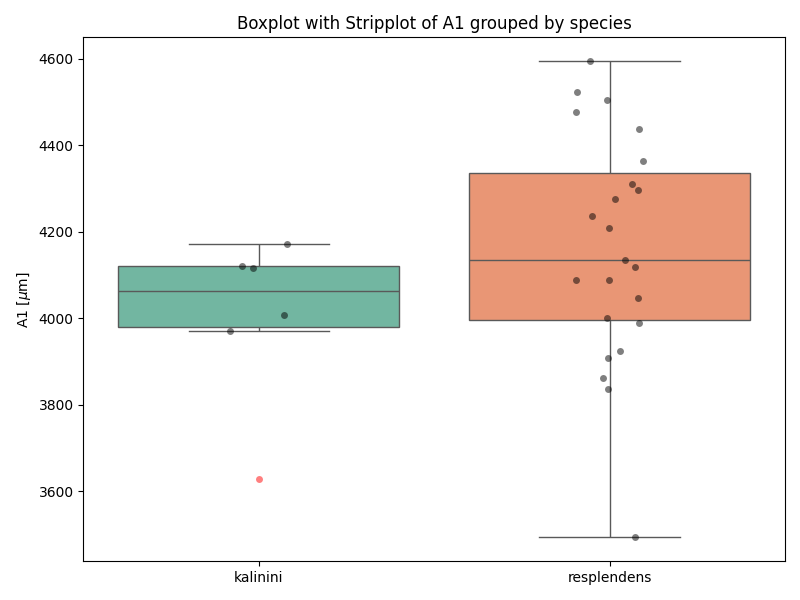
\includegraphics[width=0.7\linewidth]{images/boxplot/boxplot_A1.png}
\caption{  Boxplot and specimen distribution (superposed) for the metric  A1 by species}
\end{figure}

\noindent\textbf{Test Type:} Student's t-test \\
\noindent\textbf{Test Statistic:} -1.360 \\
\noindent\textbf{P-value:} 0.185 \\
\noindent\textbf{Interpretation:} no significant difference

\begin{figure}[H]
\centering
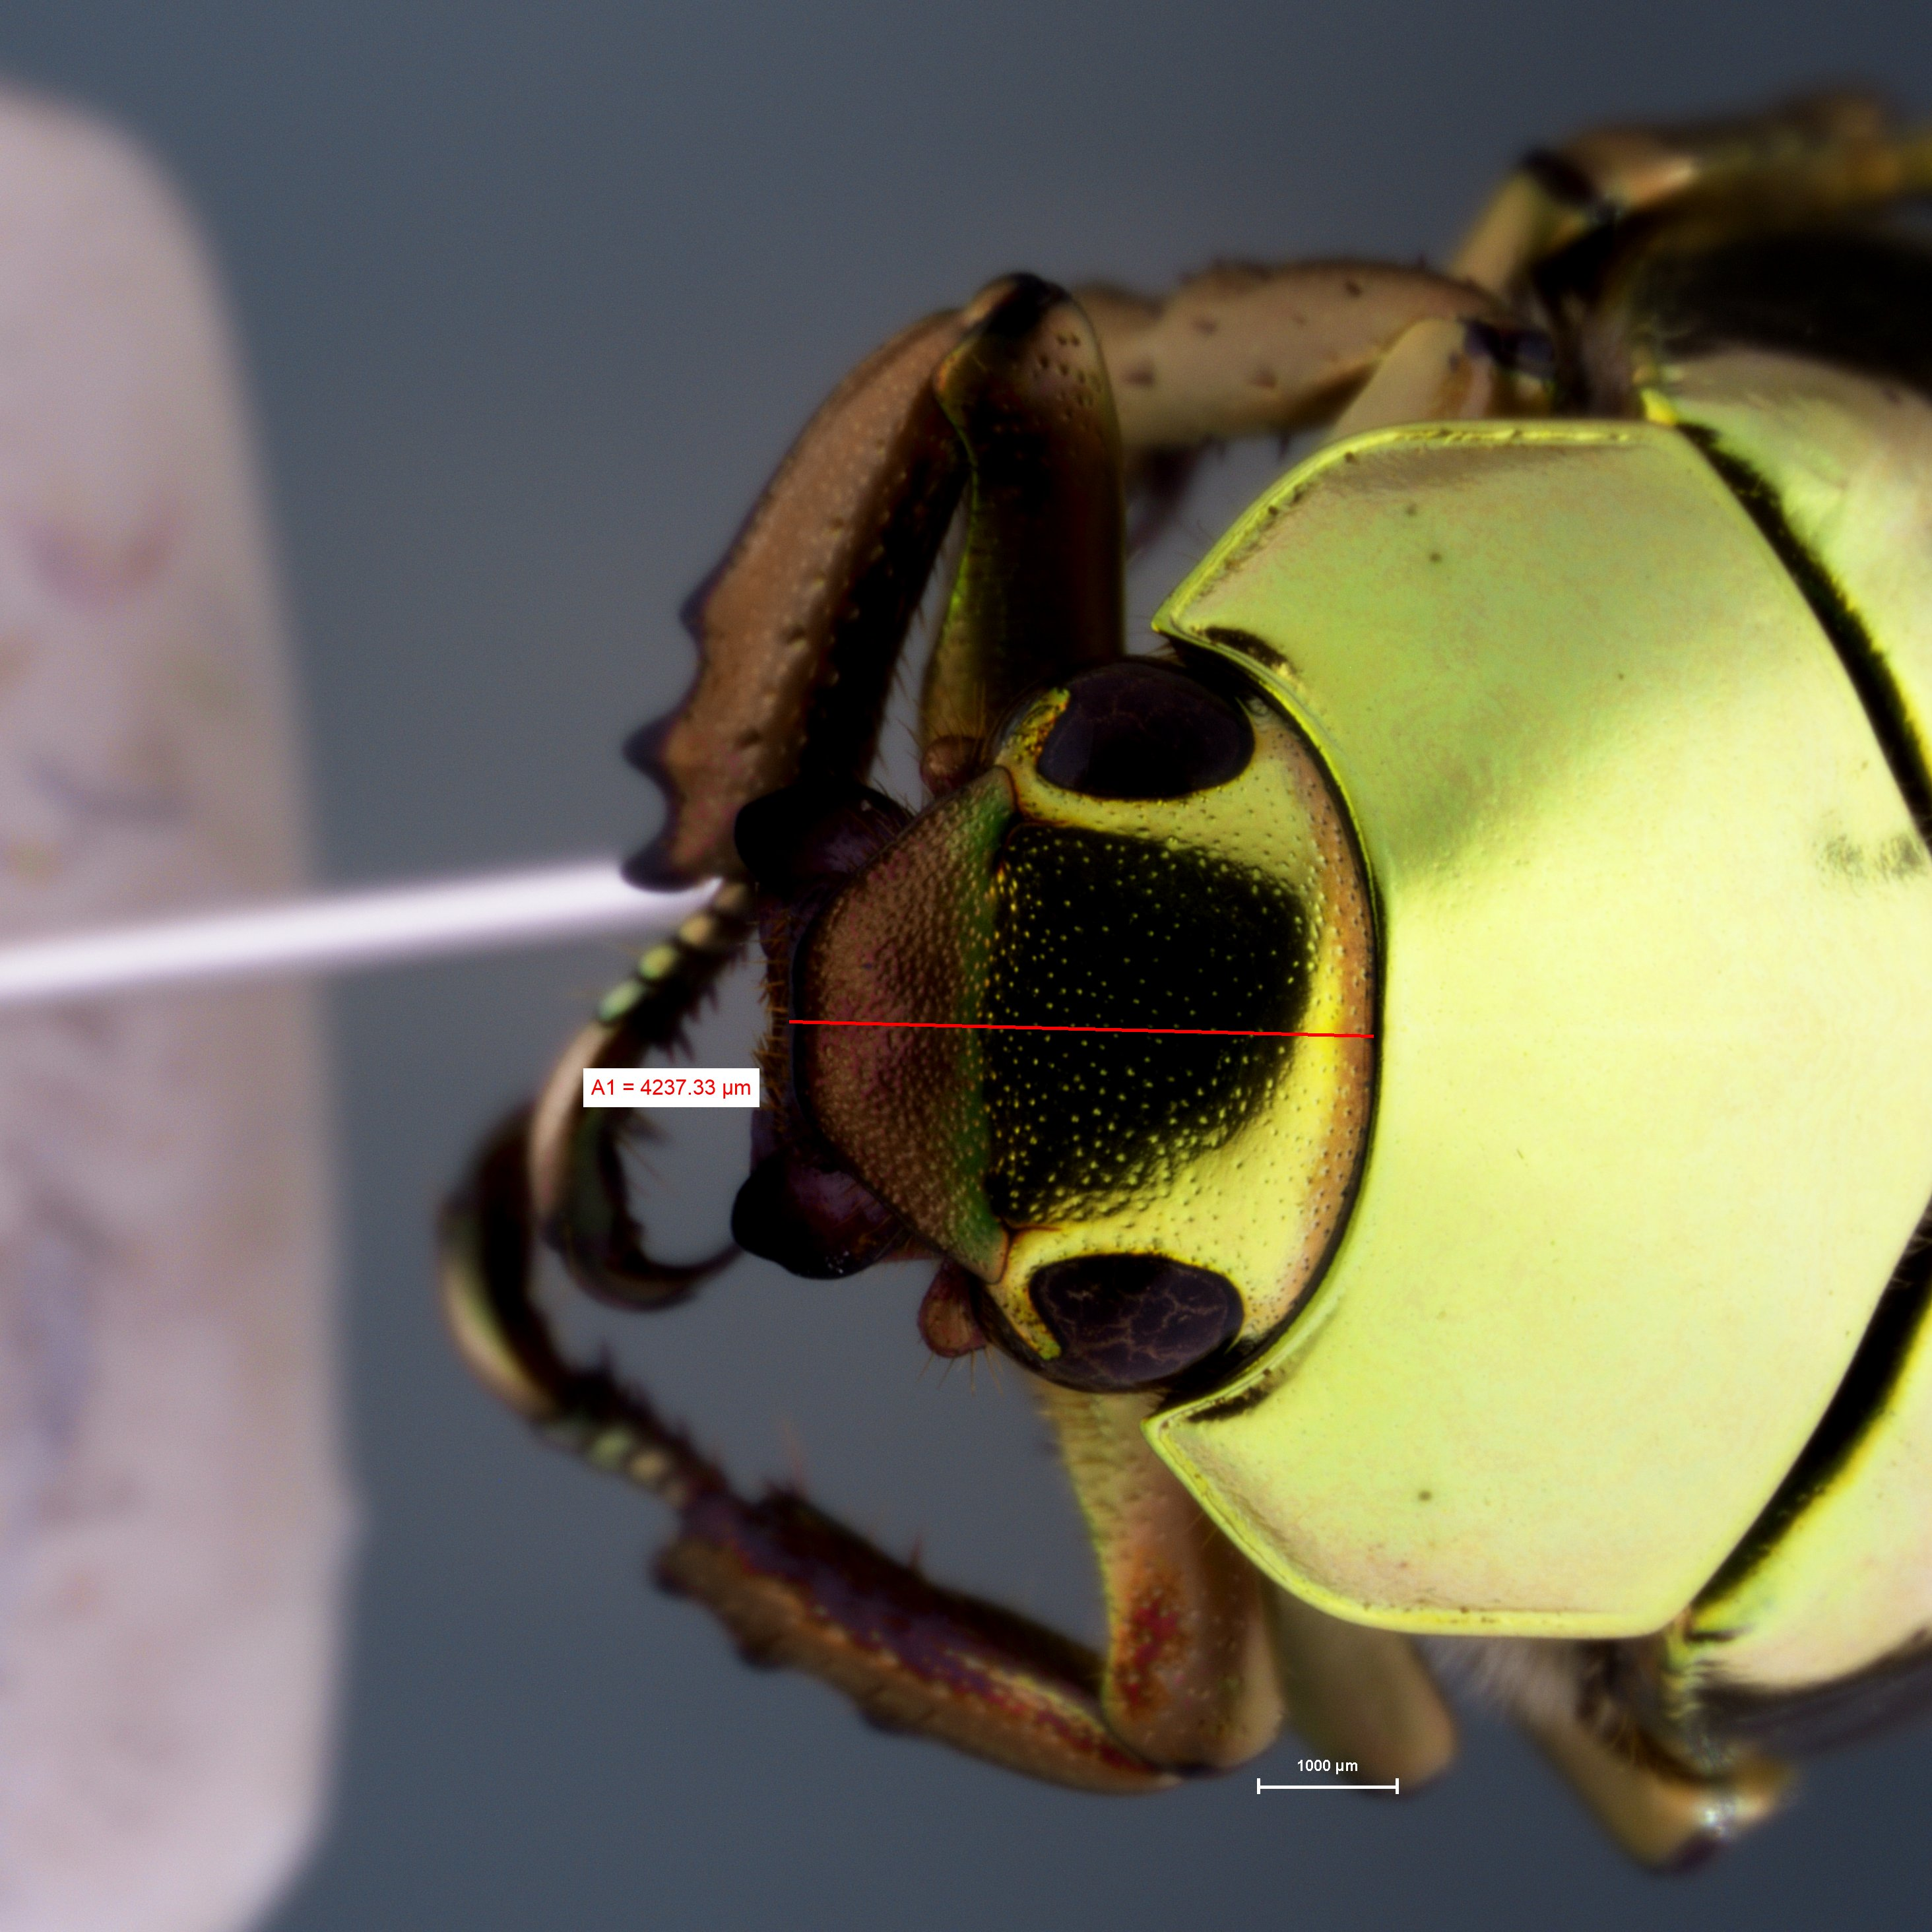
\includegraphics[width=0.5\linewidth]{images/protocol/Head_A1.png}
\caption{ Metric A1}
\end{figure}

\newpage
\subsection*{Metric: A2}

Horizontal length between the left and right sutures

\begin{figure}[H]
\centering
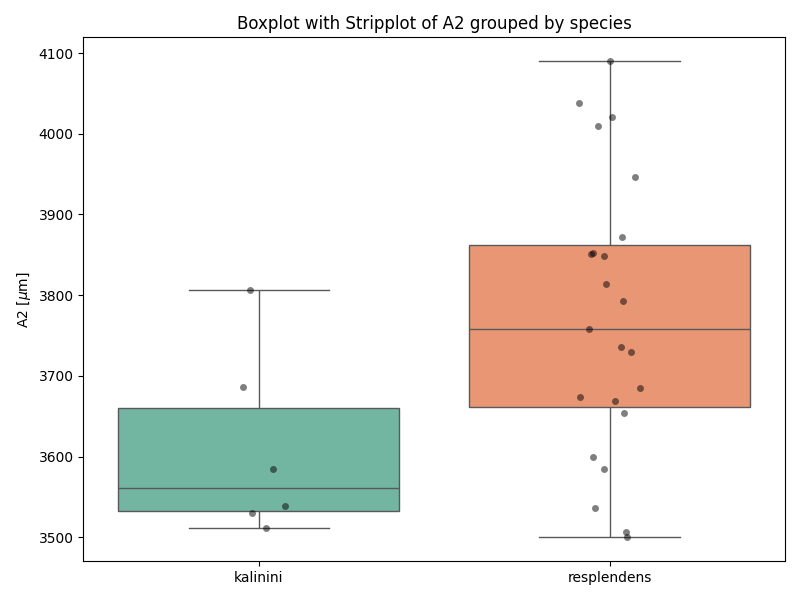
\includegraphics[width=0.7\linewidth]{images/boxplot/boxplot_A2.png}
\caption{  Boxplot and specimen distribution (superposed) for the metric  A2 by species}
\end{figure}

\noindent\textbf{Test Type:} Student's t-test \\
\noindent\textbf{Test Statistic:} -2.168 \\
\noindent\textbf{P-value:} 0.039 \\
\noindent\textbf{Interpretation:} significant difference

\begin{figure}[H]
\centering
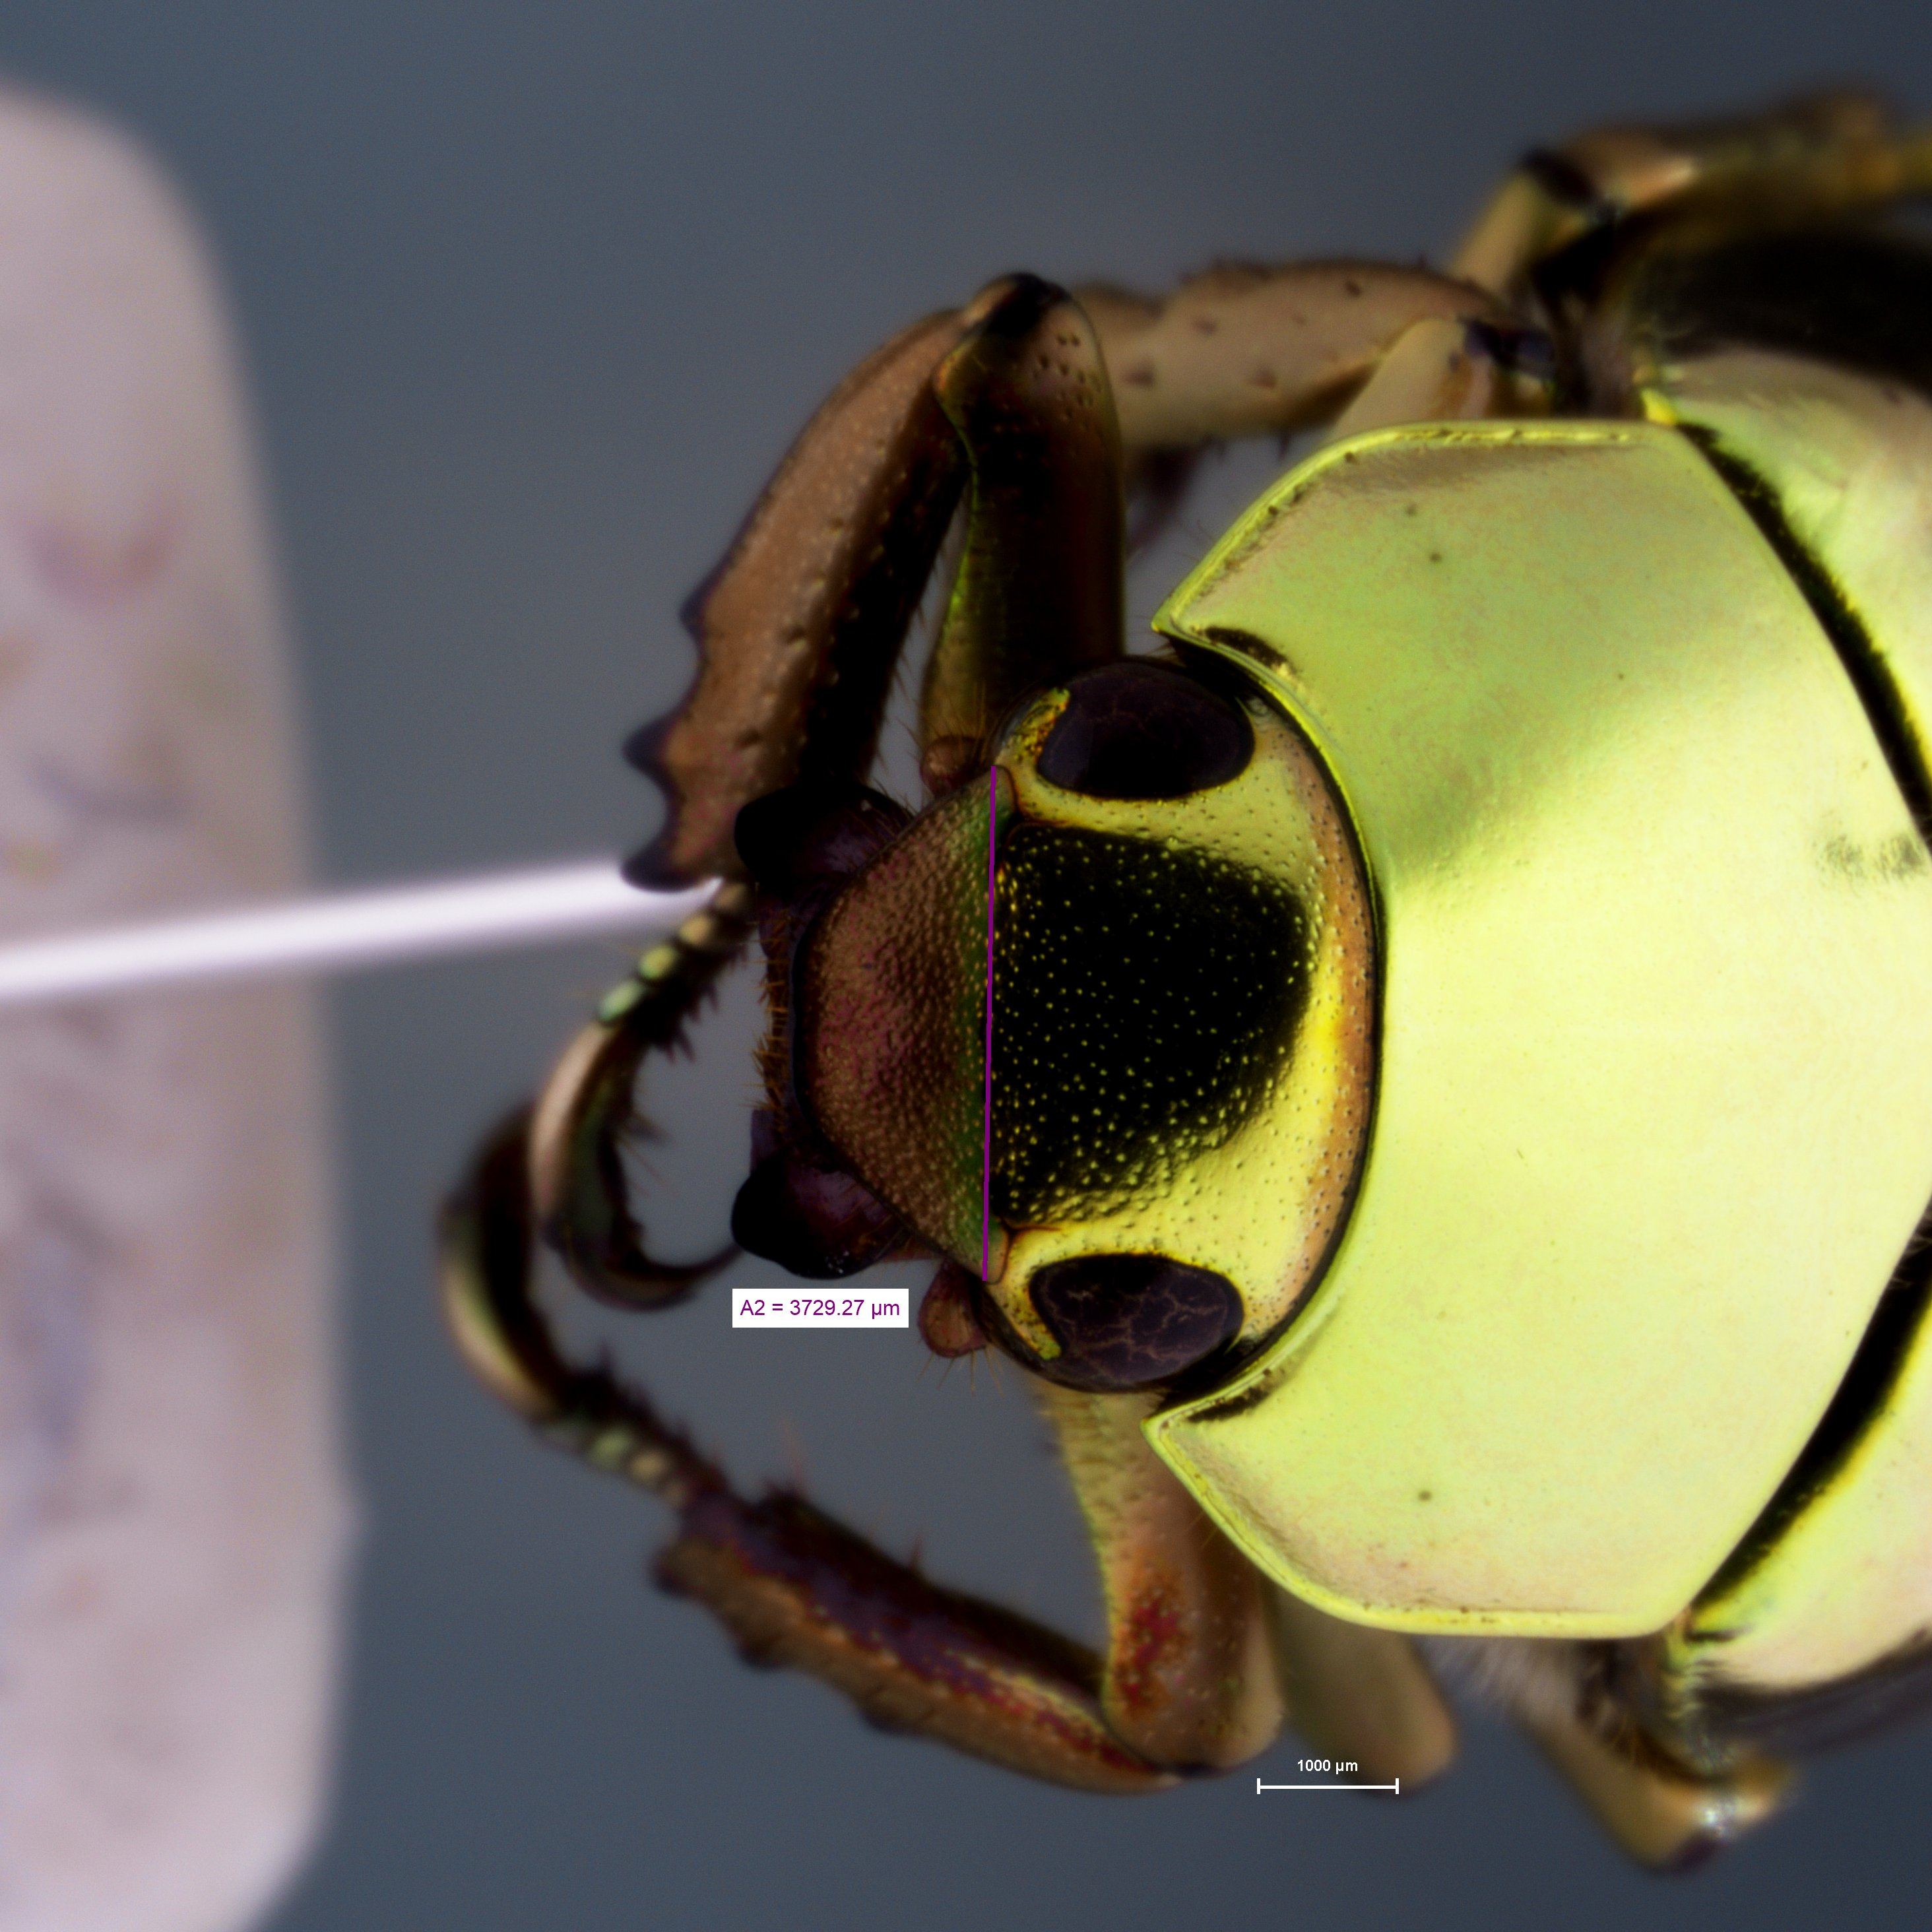
\includegraphics[width=0.5\linewidth]{images/protocol/Head_A2.png}
\caption{ Metric A2}
\end{figure}

\newpage
\subsection*{Metric: A3}

Horizontal length between the left and right eye’s canthus

\begin{figure}[H]
\centering
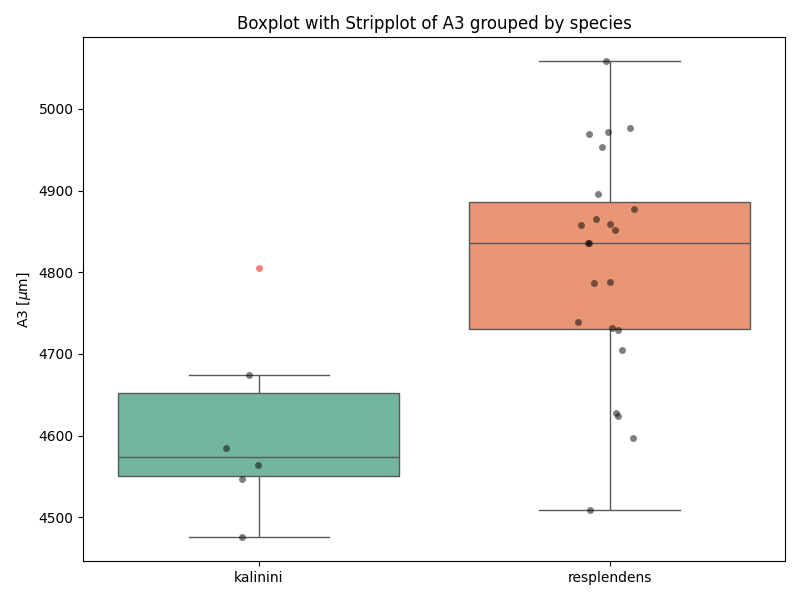
\includegraphics[width=0.7\linewidth]{images/boxplot/boxplot_A3.png}
\caption{  Boxplot and specimen distribution (superposed) for the metric  A3 by species}
\end{figure}

\noindent\textbf{Test Type:} Student's t-test \\
\noindent\textbf{Test Statistic:} -3.297 \\
\noindent\textbf{P-value:} 0.003 \\
\noindent\textbf{Interpretation:} significant difference

\begin{figure}[H]
\centering
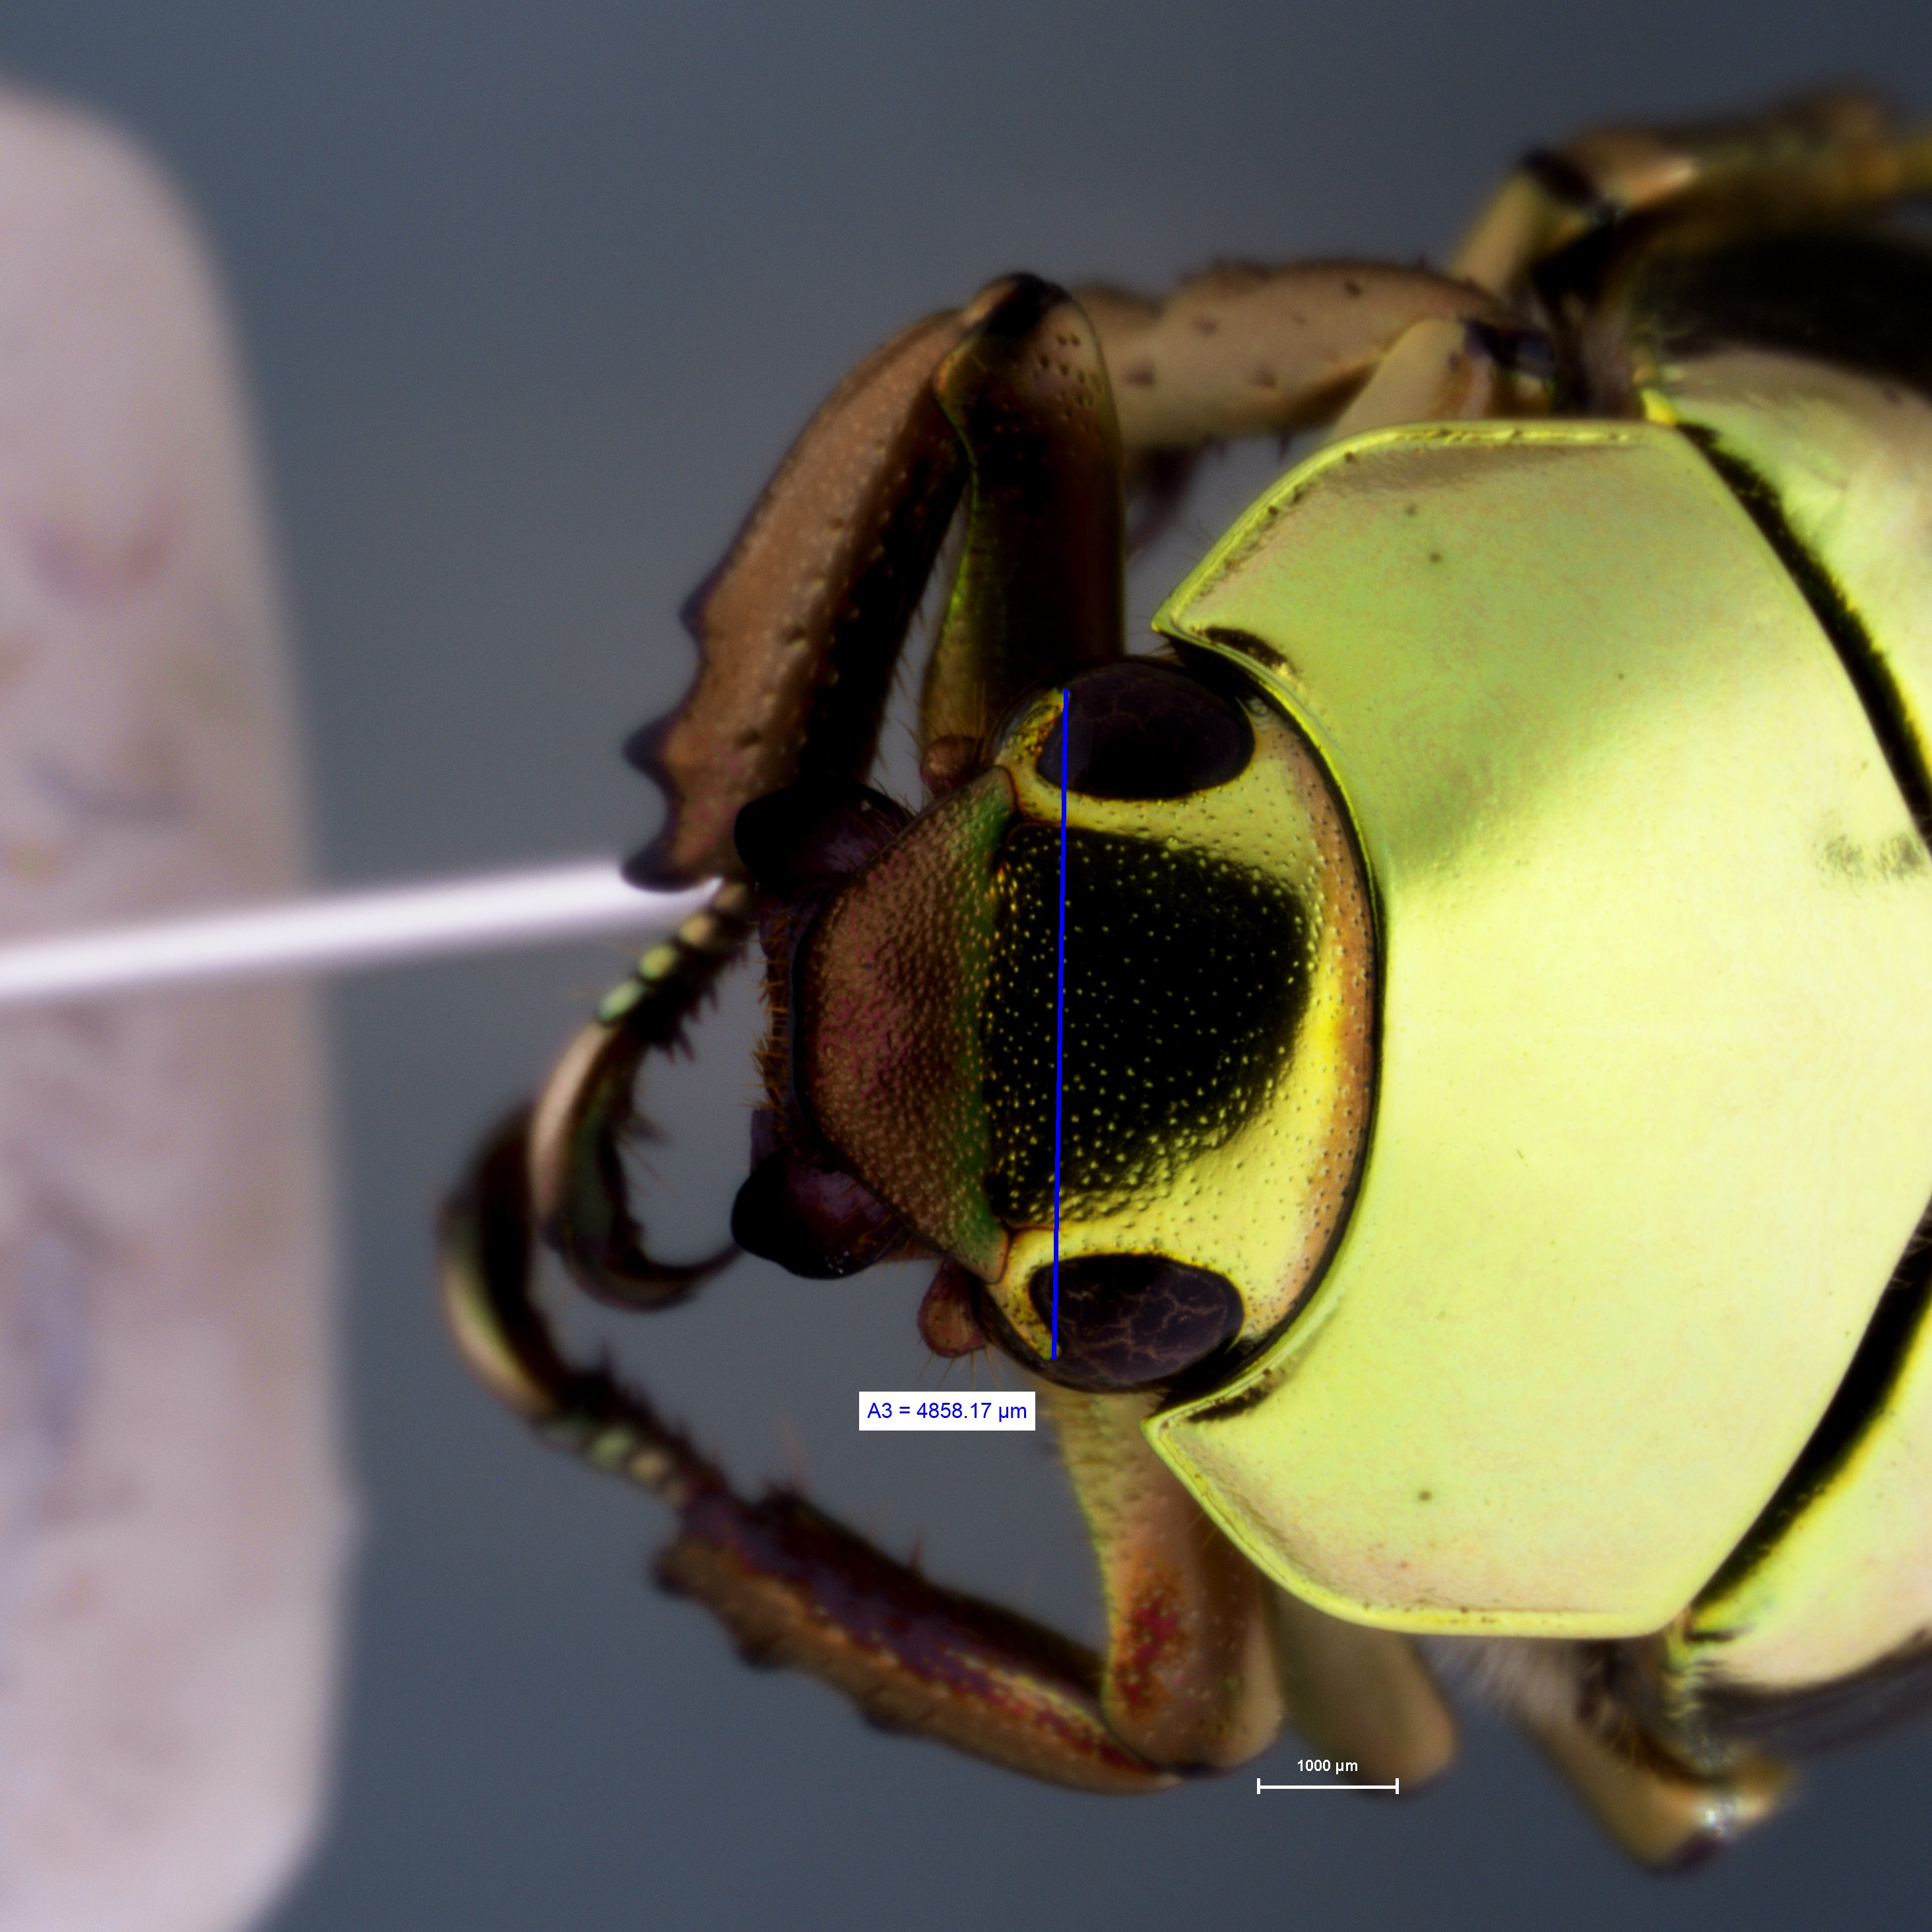
\includegraphics[width=0.5\linewidth]{images/protocol/Head_A3.png}
\caption{ Metric A3}
\end{figure}

\newpage
\subsection*{Metric: A4}

Vertical ortogonal length of the clipeus measured from the front down to A2 line

\begin{figure}[H]
\centering
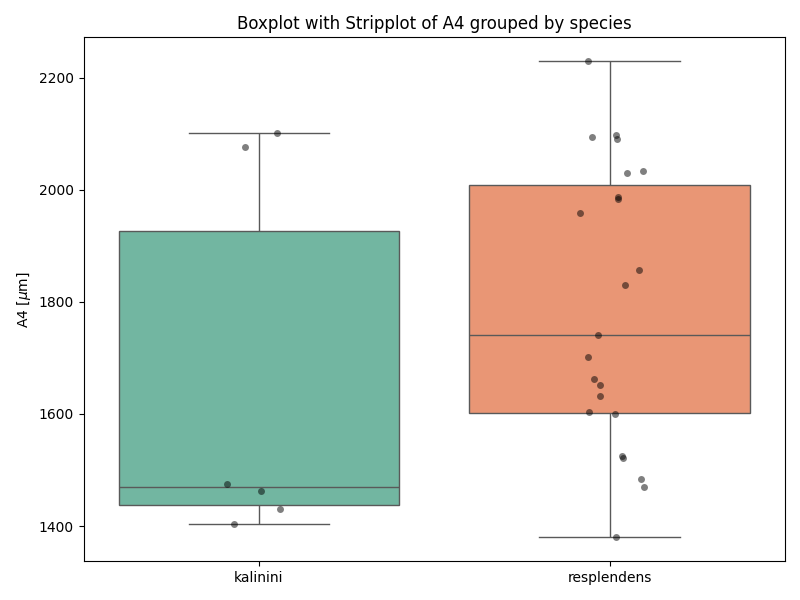
\includegraphics[width=0.7\linewidth]{images/boxplot/boxplot_A4.png}
\caption{  Boxplot and specimen distribution (superposed) for the metric  A4 by species}
\end{figure}

\noindent\textbf{Test Type:} Mann-Whitney U test \\
\noindent\textbf{Test Statistic:} 46.000 \\
\noindent\textbf{P-value:} 0.232 \\
\noindent\textbf{Interpretation:} no significant difference

\begin{figure}[H]
\centering
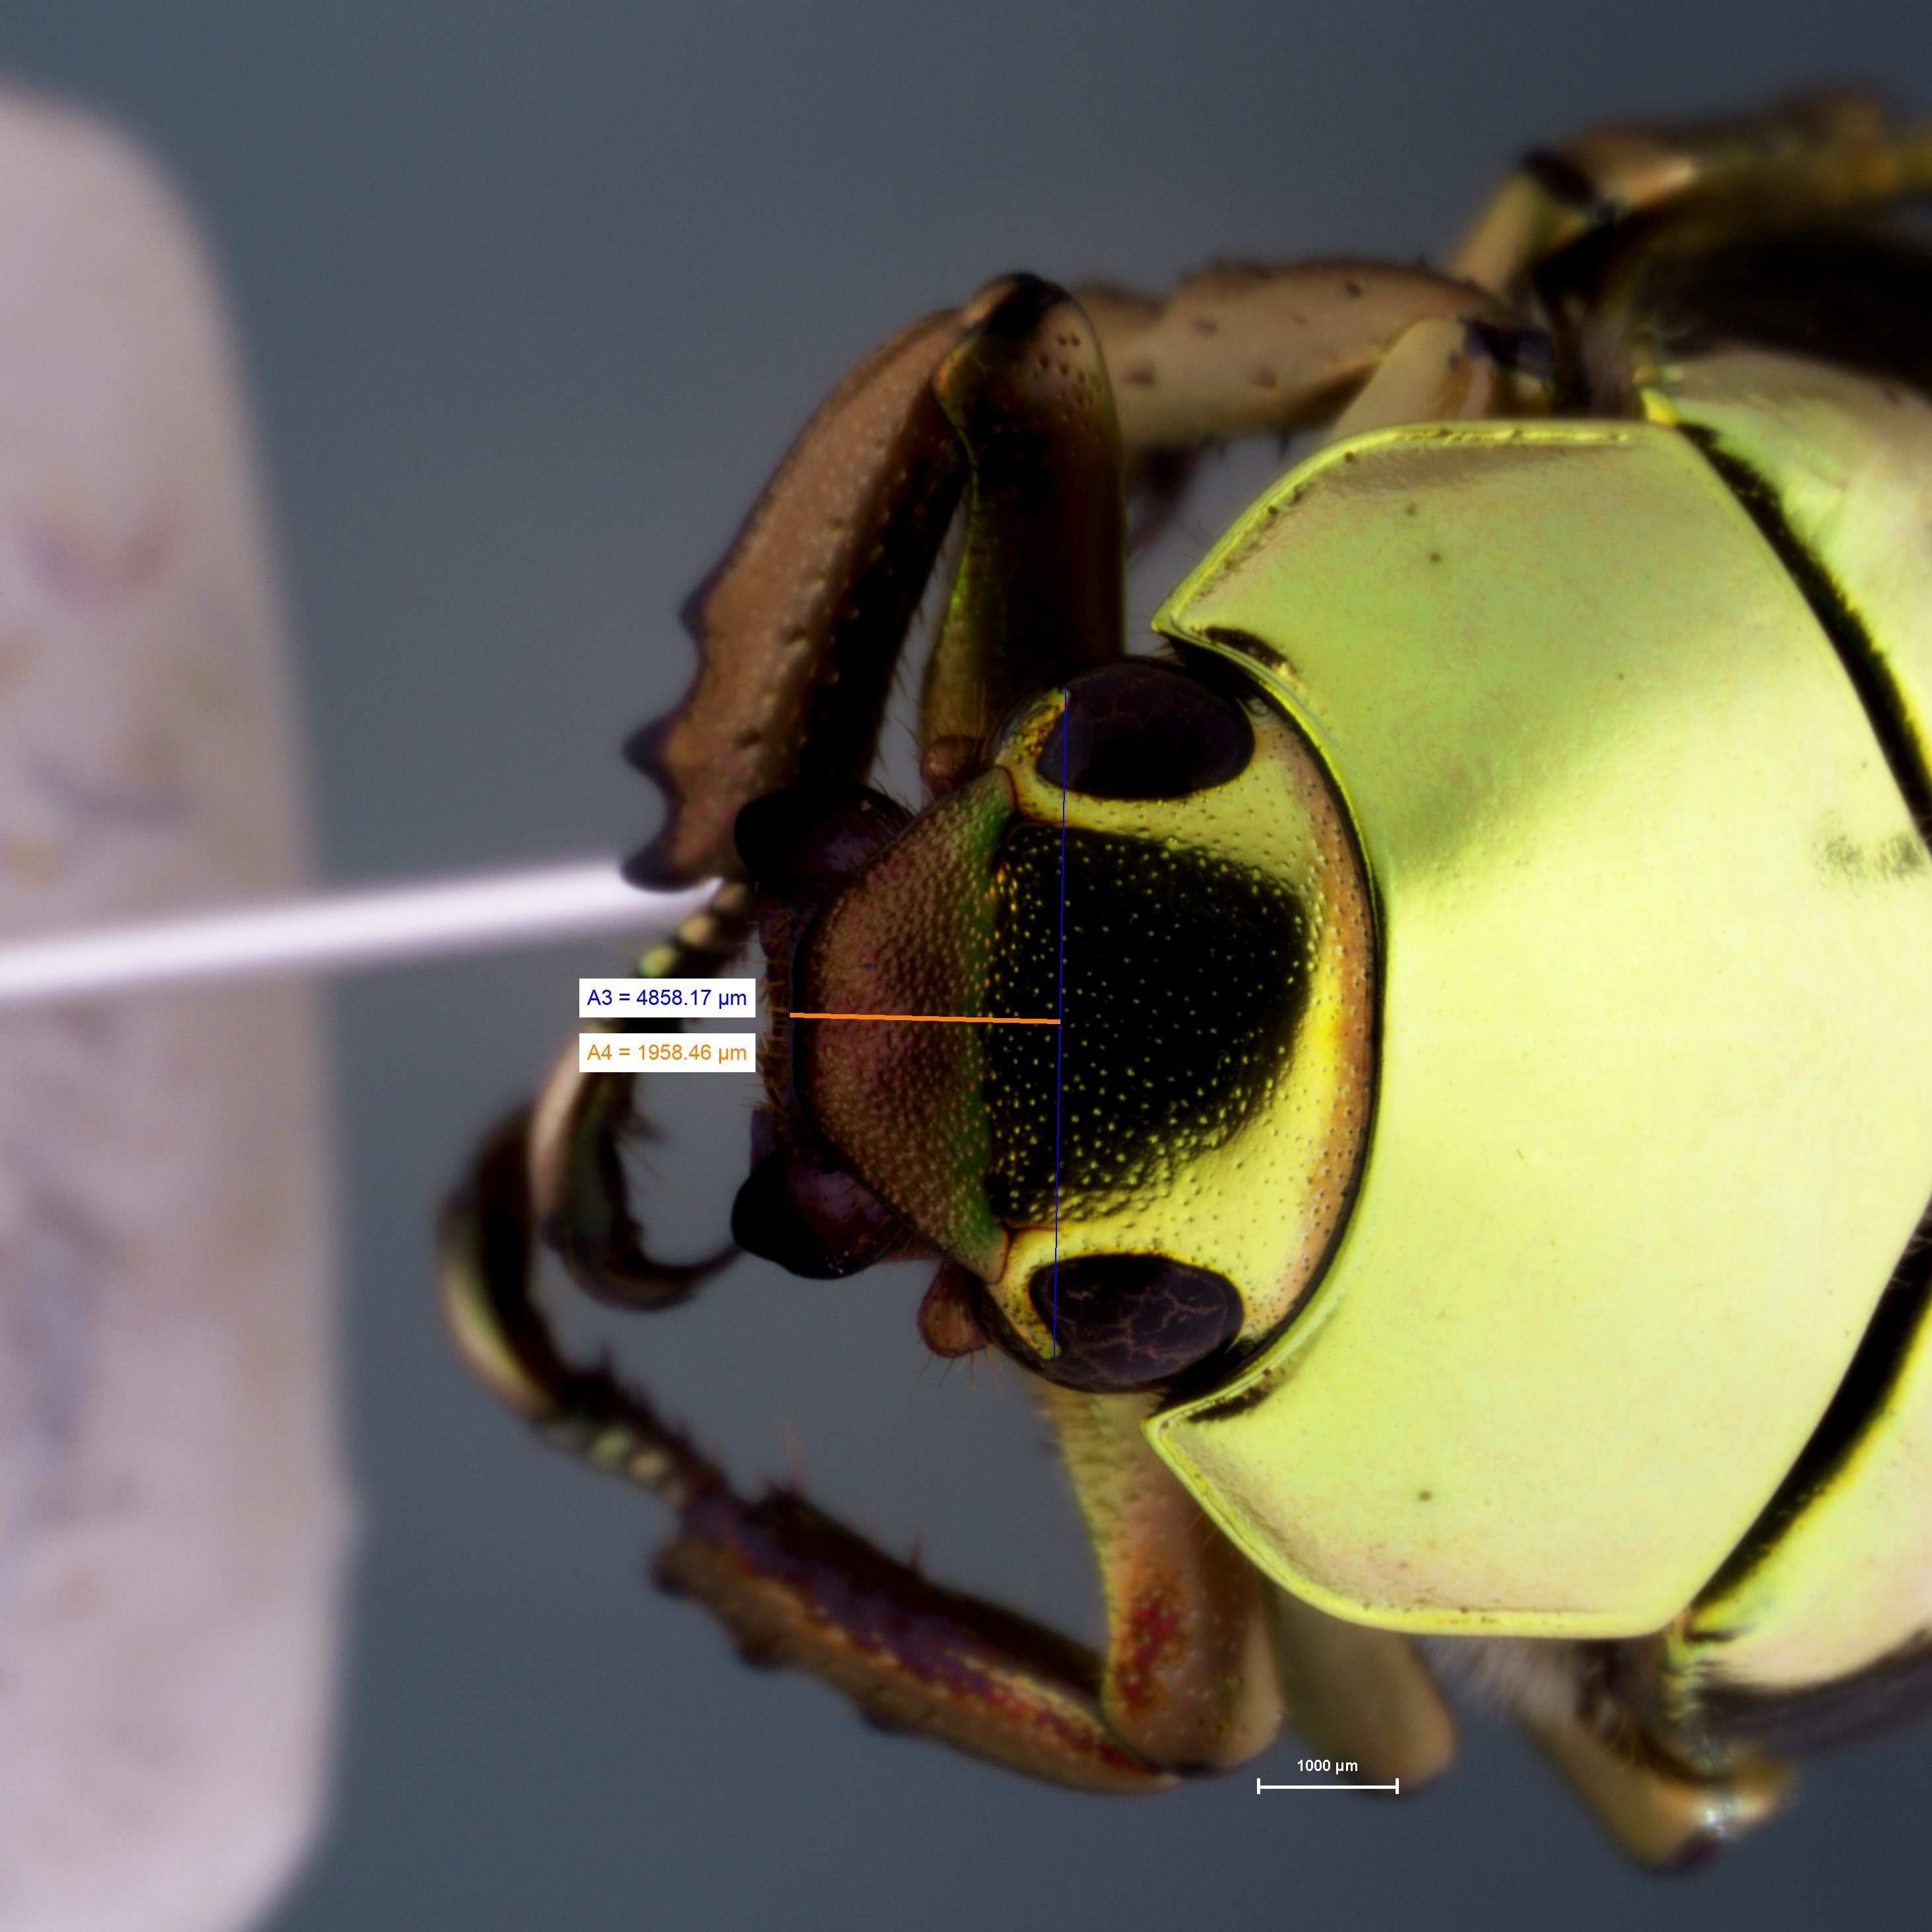
\includegraphics[width=0.5\linewidth]{images/protocol/Head_A4.png}
\caption{ Metric A4}
\end{figure}

\newpage
\subsection*{Metric: A5}

Perpendicular vertical length of the clypeus, measured from its front edge to the $A2$ line, representing the clypeus height.

\begin{figure}[H]
\centering
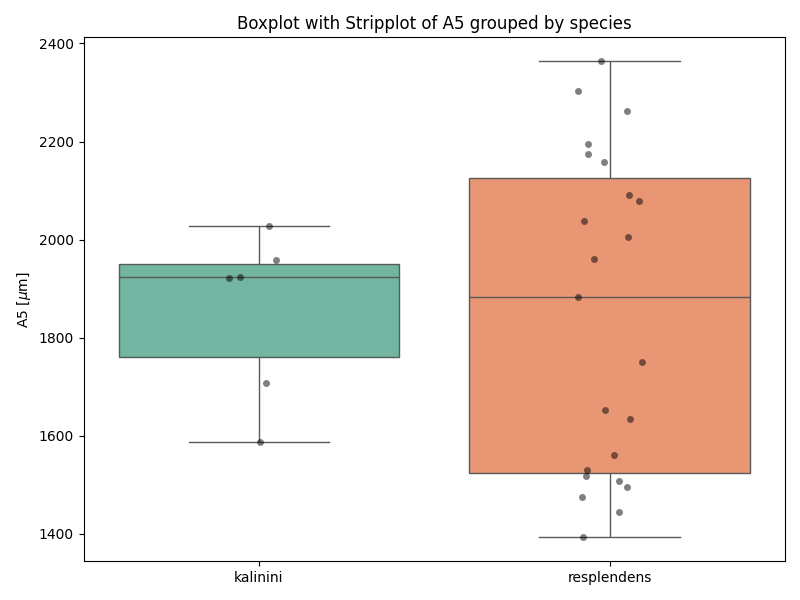
\includegraphics[width=0.7\linewidth]{images/boxplot/boxplot_A5.png}
\caption{  Boxplot and specimen distribution (superposed) for the metric  A5 by species}
\end{figure}

\noindent\textbf{Test Type:} Mann-Whitney U test \\
\noindent\textbf{Test Statistic:} 68.000 \\
\noindent\textbf{P-value:} 0.979 \\
\noindent\textbf{Interpretation:} no significant difference

\begin{figure}[H]
\centering
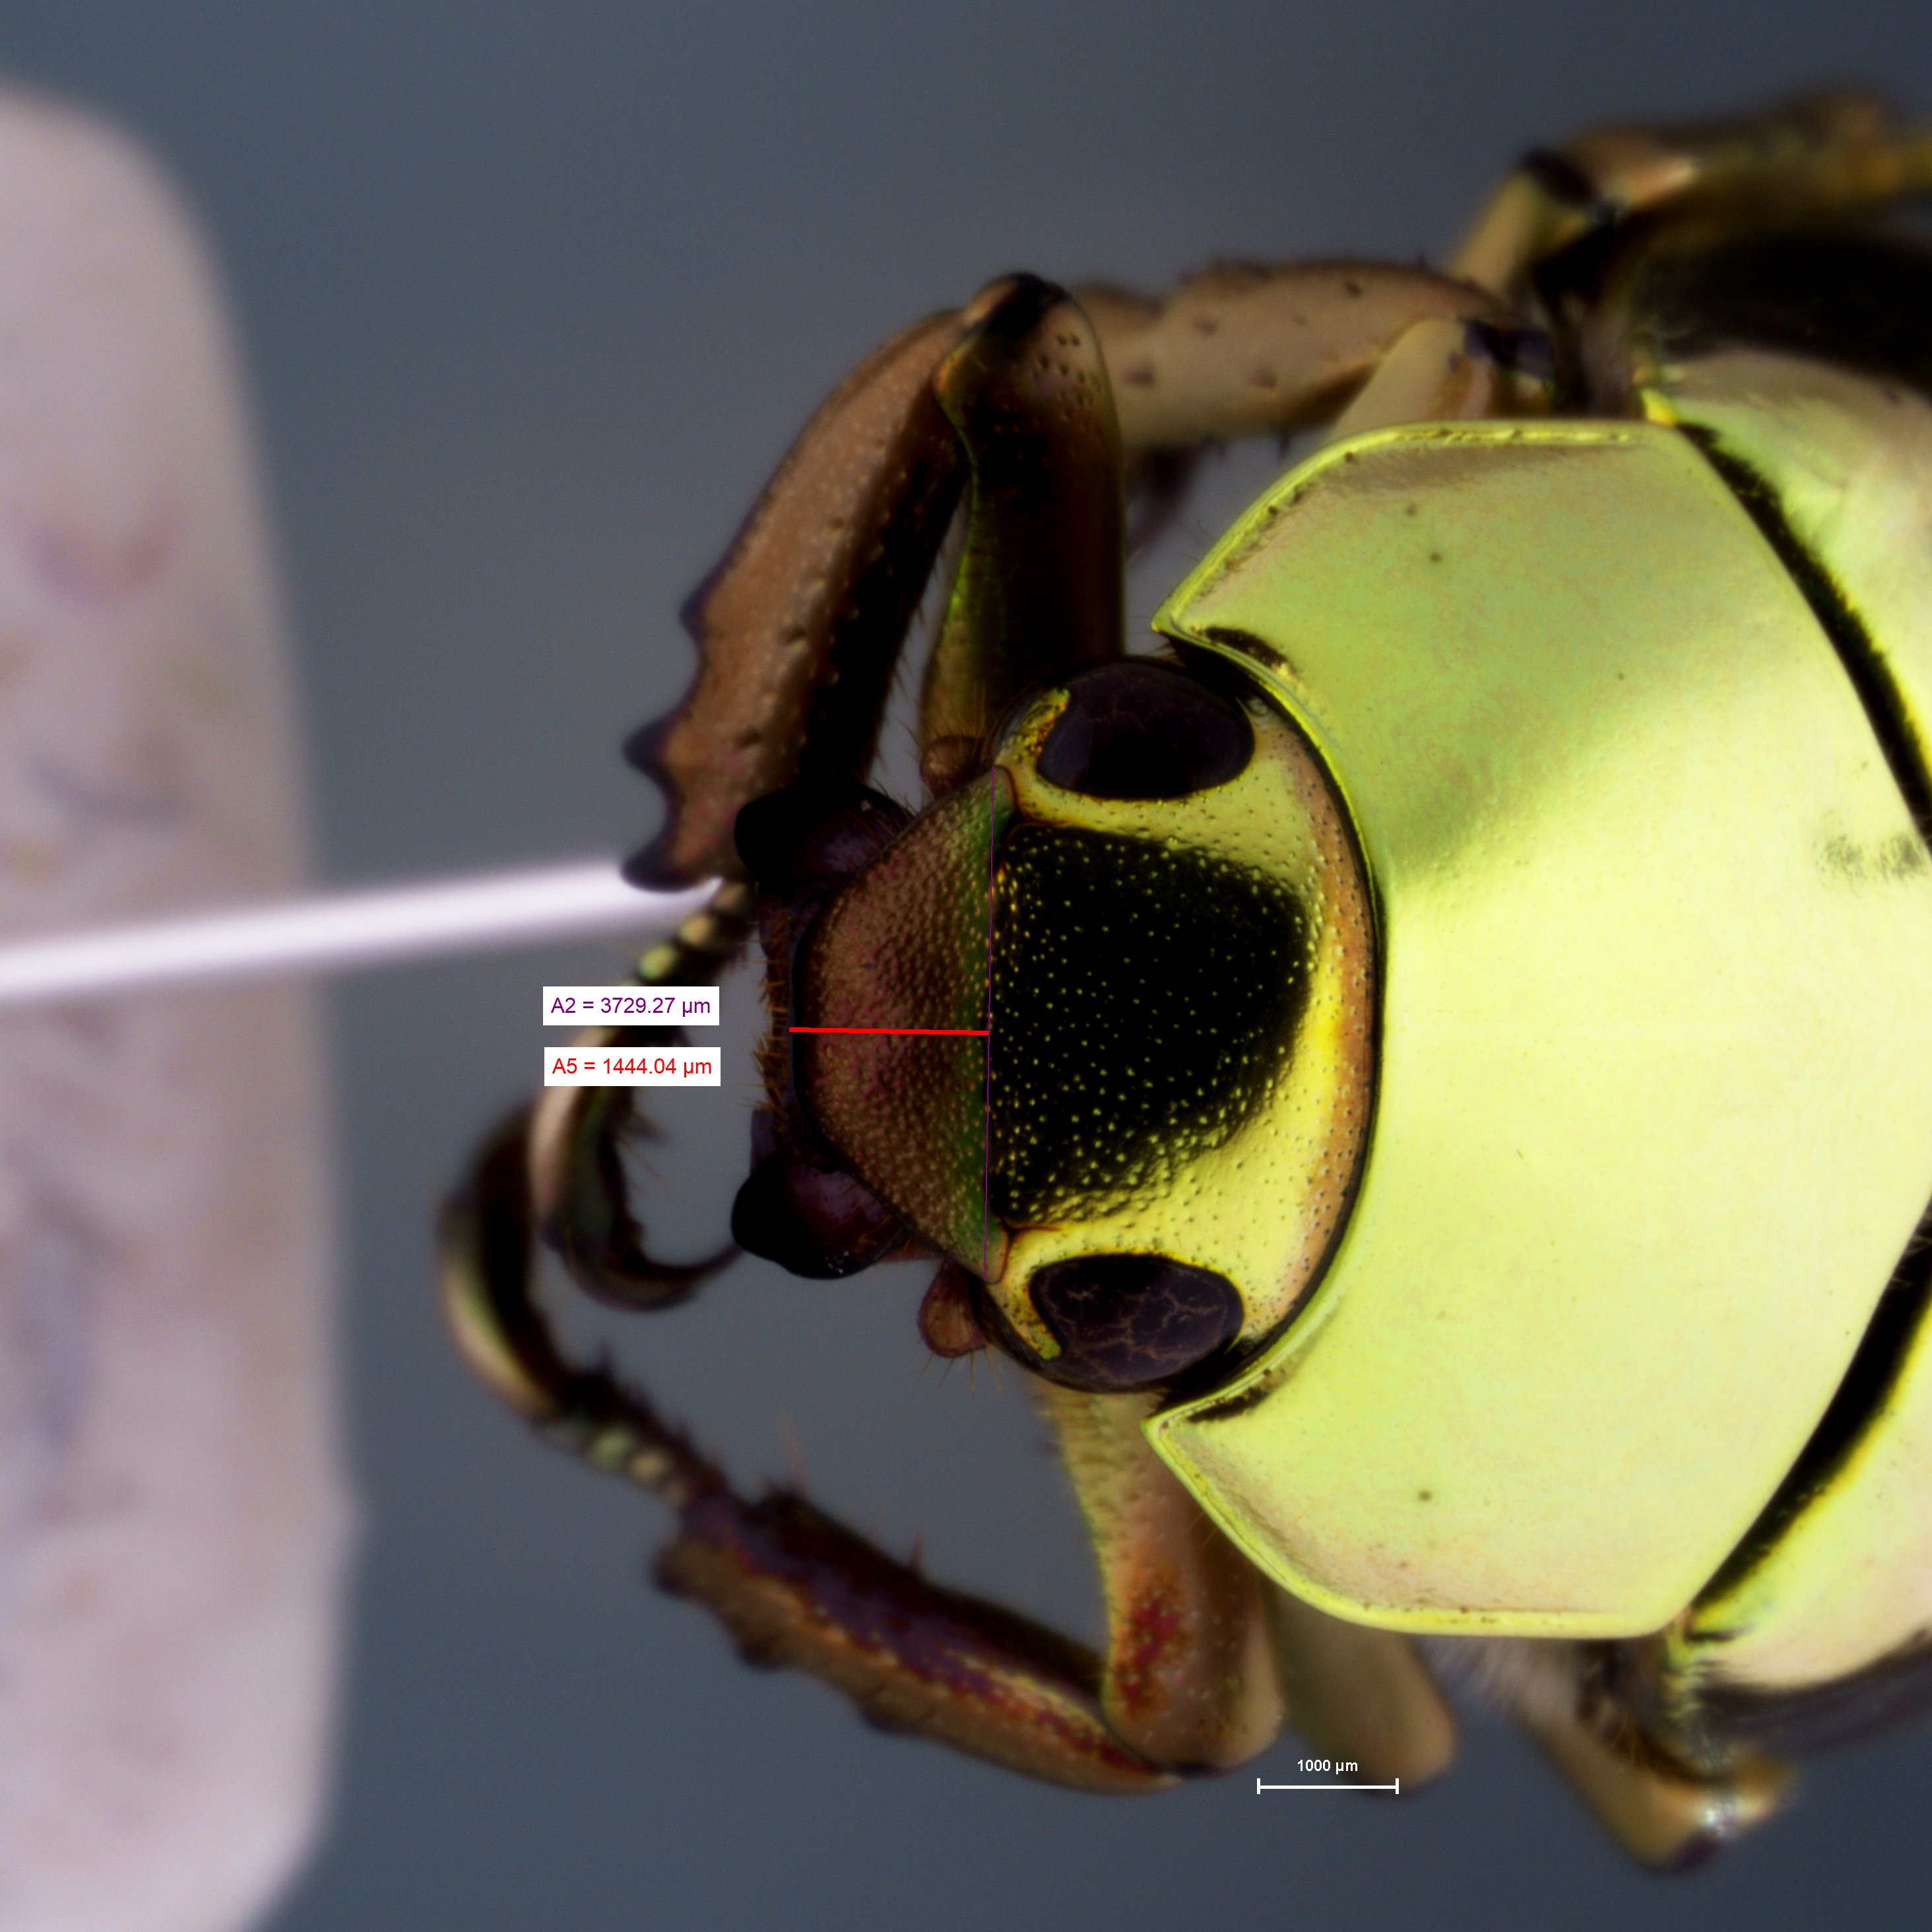
\includegraphics[width=0.5\linewidth]{images/protocol/Head_A5.png}
\caption{ Metric A5}
\end{figure}

\newpage
\subsection*{Metric: B1}

Horizontal length between the pronotum’s frontal angles

\begin{figure}[H]
\centering
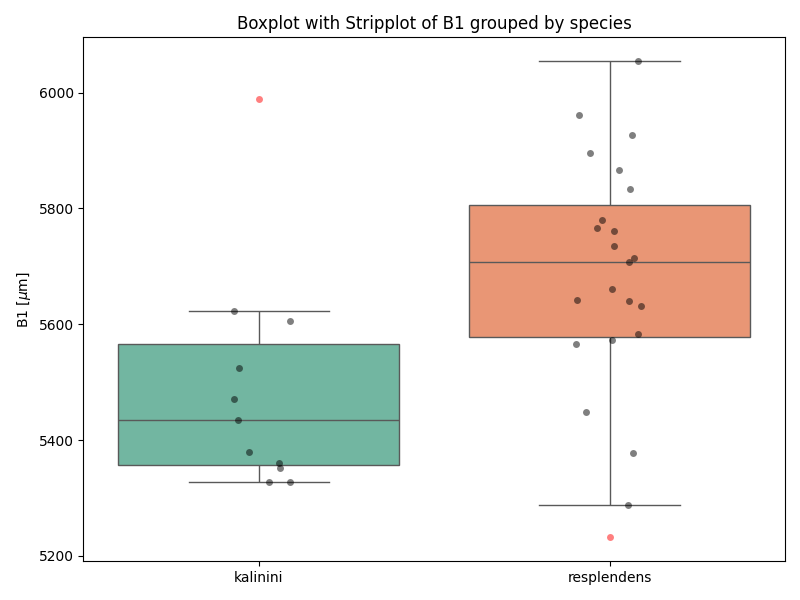
\includegraphics[width=0.7\linewidth]{images/boxplot/boxplot_B1.png}
\caption{  Boxplot and specimen distribution (superposed) for the metric  B1 by species}
\end{figure}

\noindent\textbf{Test Type:} Mann-Whitney U test \\
\noindent\textbf{Test Statistic:} 58.000 \\
\noindent\textbf{P-value:} 0.012 \\
\noindent\textbf{Interpretation:} significant difference

\begin{figure}[H]
\centering
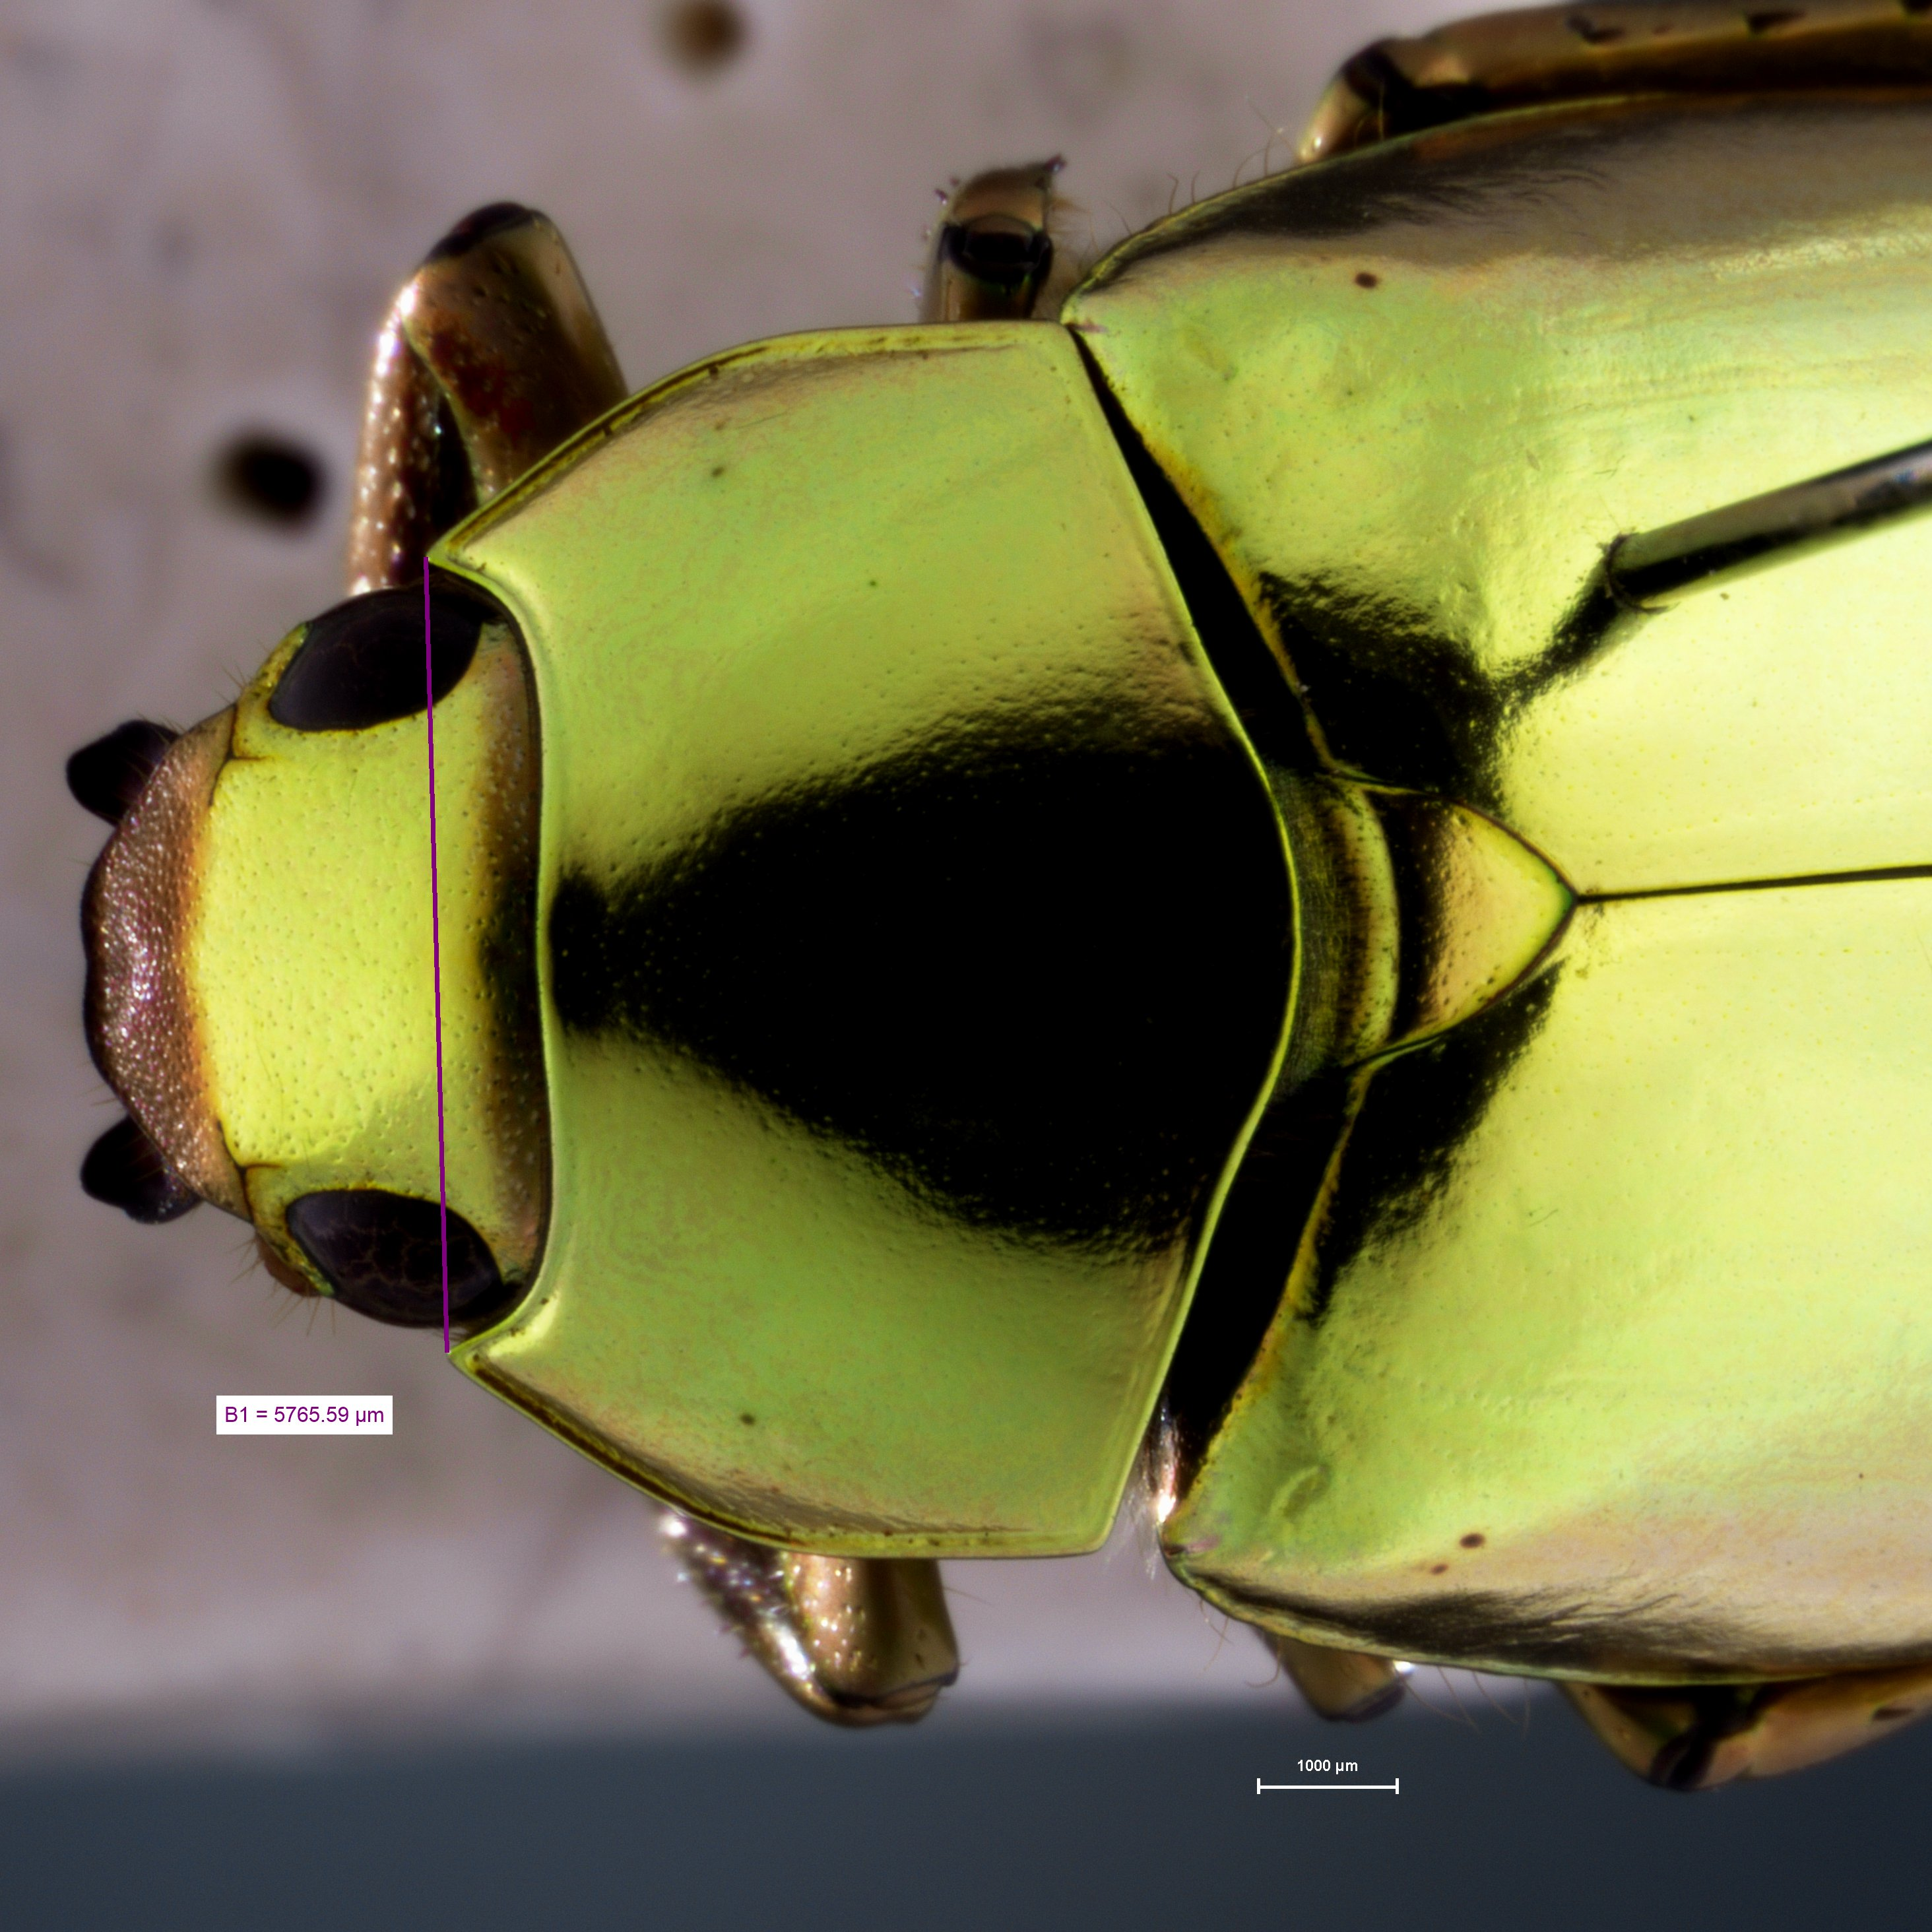
\includegraphics[width=0.5\linewidth]{images/protocol/Pronotum_B1.png}
\caption{ Metric B1}
\end{figure}

\newpage
\subsection*{Metric: B2}

Horizontal length between the pronotum’s middle angles

\begin{figure}[H]
\centering
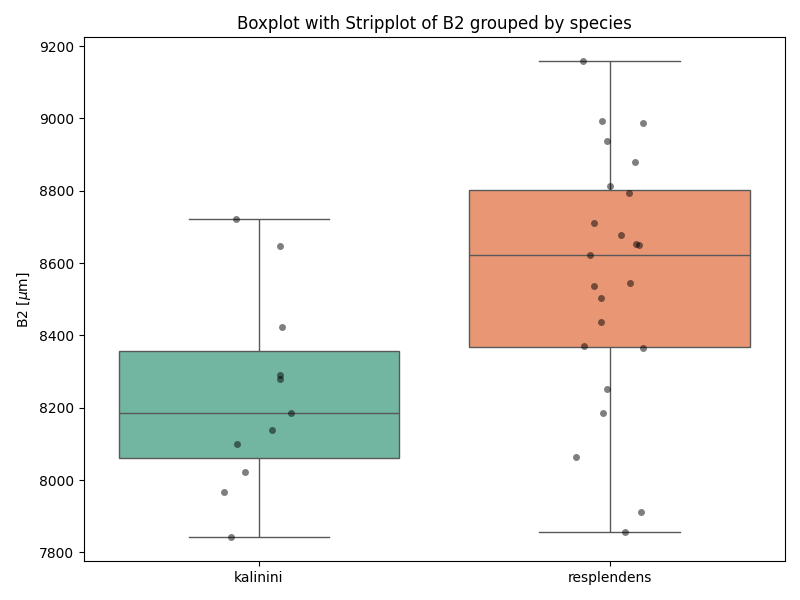
\includegraphics[width=0.7\linewidth]{images/boxplot/boxplot_B2.png}
\caption{  Boxplot and specimen distribution (superposed) for the metric  B2 by species}
\end{figure}

\noindent\textbf{Test Type:} Student's t-test \\
\noindent\textbf{Test Statistic:} -2.710 \\
\noindent\textbf{P-value:} 0.011 \\
\noindent\textbf{Interpretation:} significant difference

\begin{figure}[H]
\centering
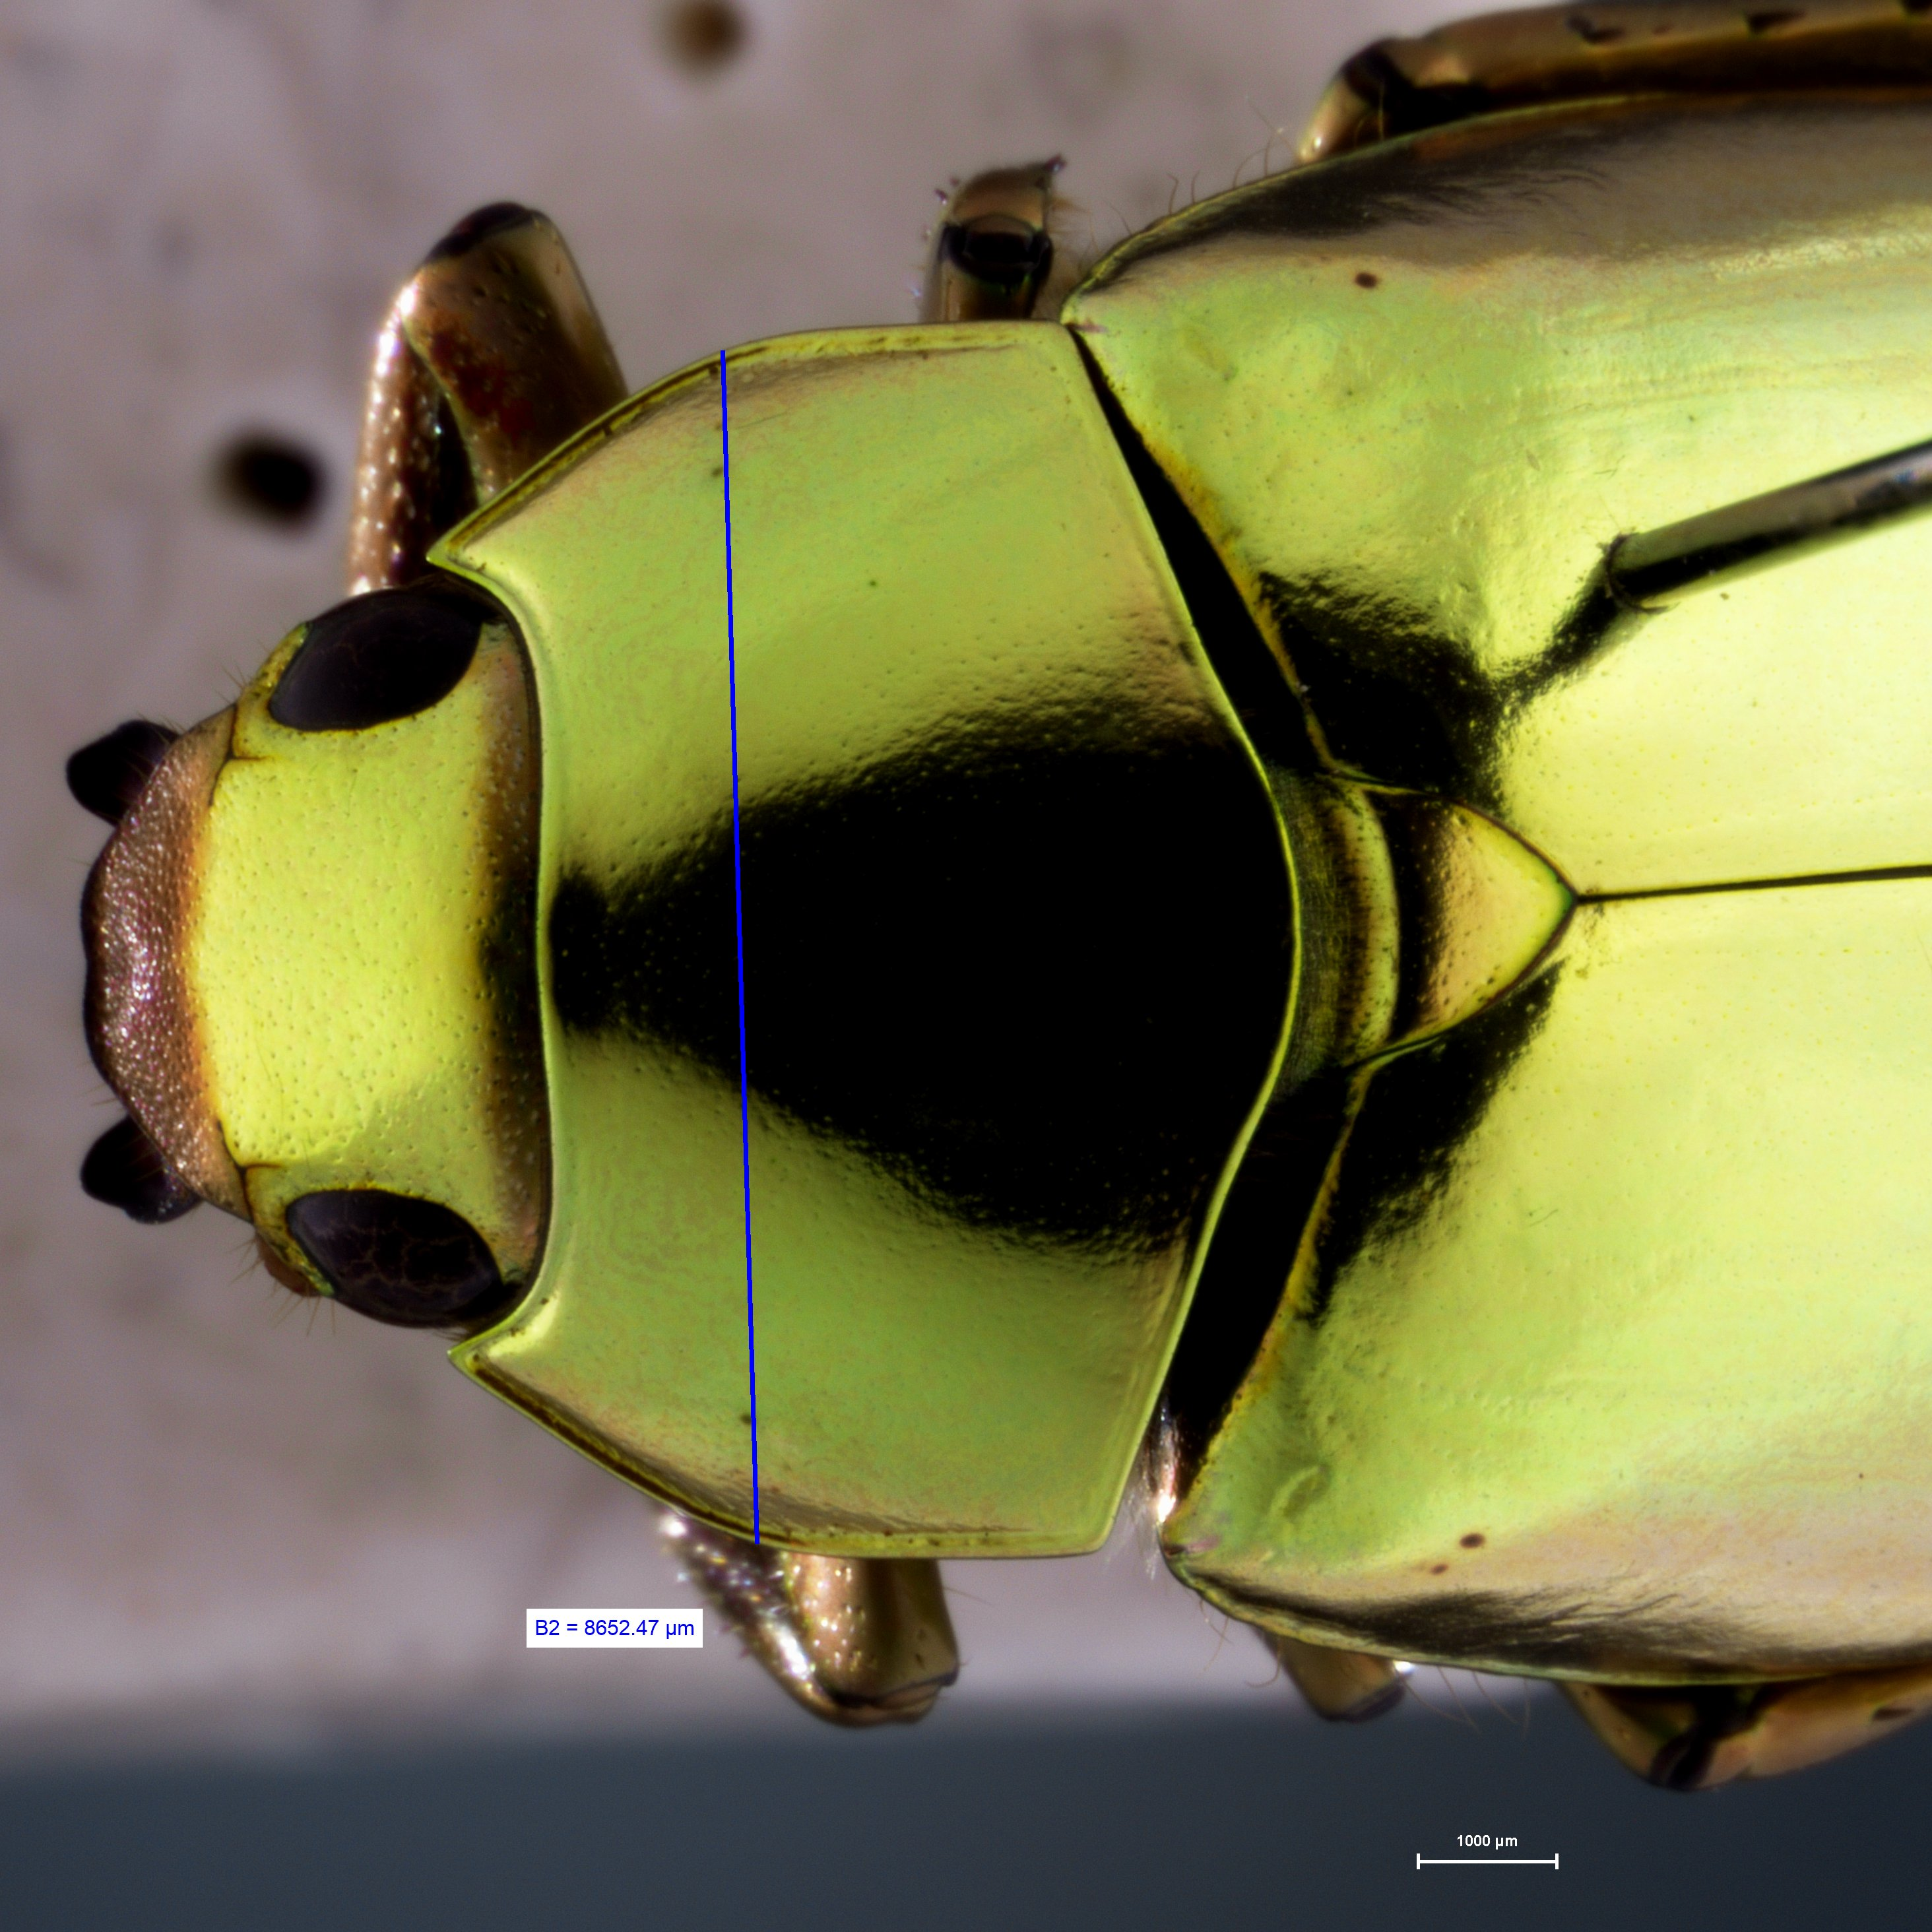
\includegraphics[width=0.5\linewidth]{images/protocol/Pronotum_B2.png}
\caption{ Metric B2}
\end{figure}

\newpage
\subsection*{Metric: B3}

Horizontal length between the pronotum’s hind angles

\begin{figure}[H]
\centering
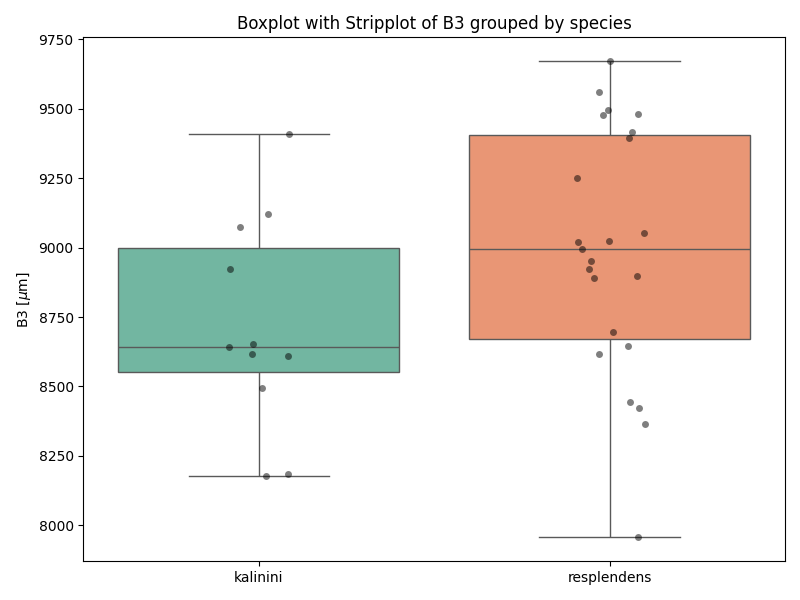
\includegraphics[width=0.7\linewidth]{images/boxplot/boxplot_B3.png}
\caption{  Boxplot and specimen distribution (superposed) for the metric  B3 by species}
\end{figure}

\noindent\textbf{Test Type:} Student's t-test \\
\noindent\textbf{Test Statistic:} -1.697 \\
\noindent\textbf{P-value:} 0.099 \\
\noindent\textbf{Interpretation:} no significant difference

\begin{figure}[H]
\centering
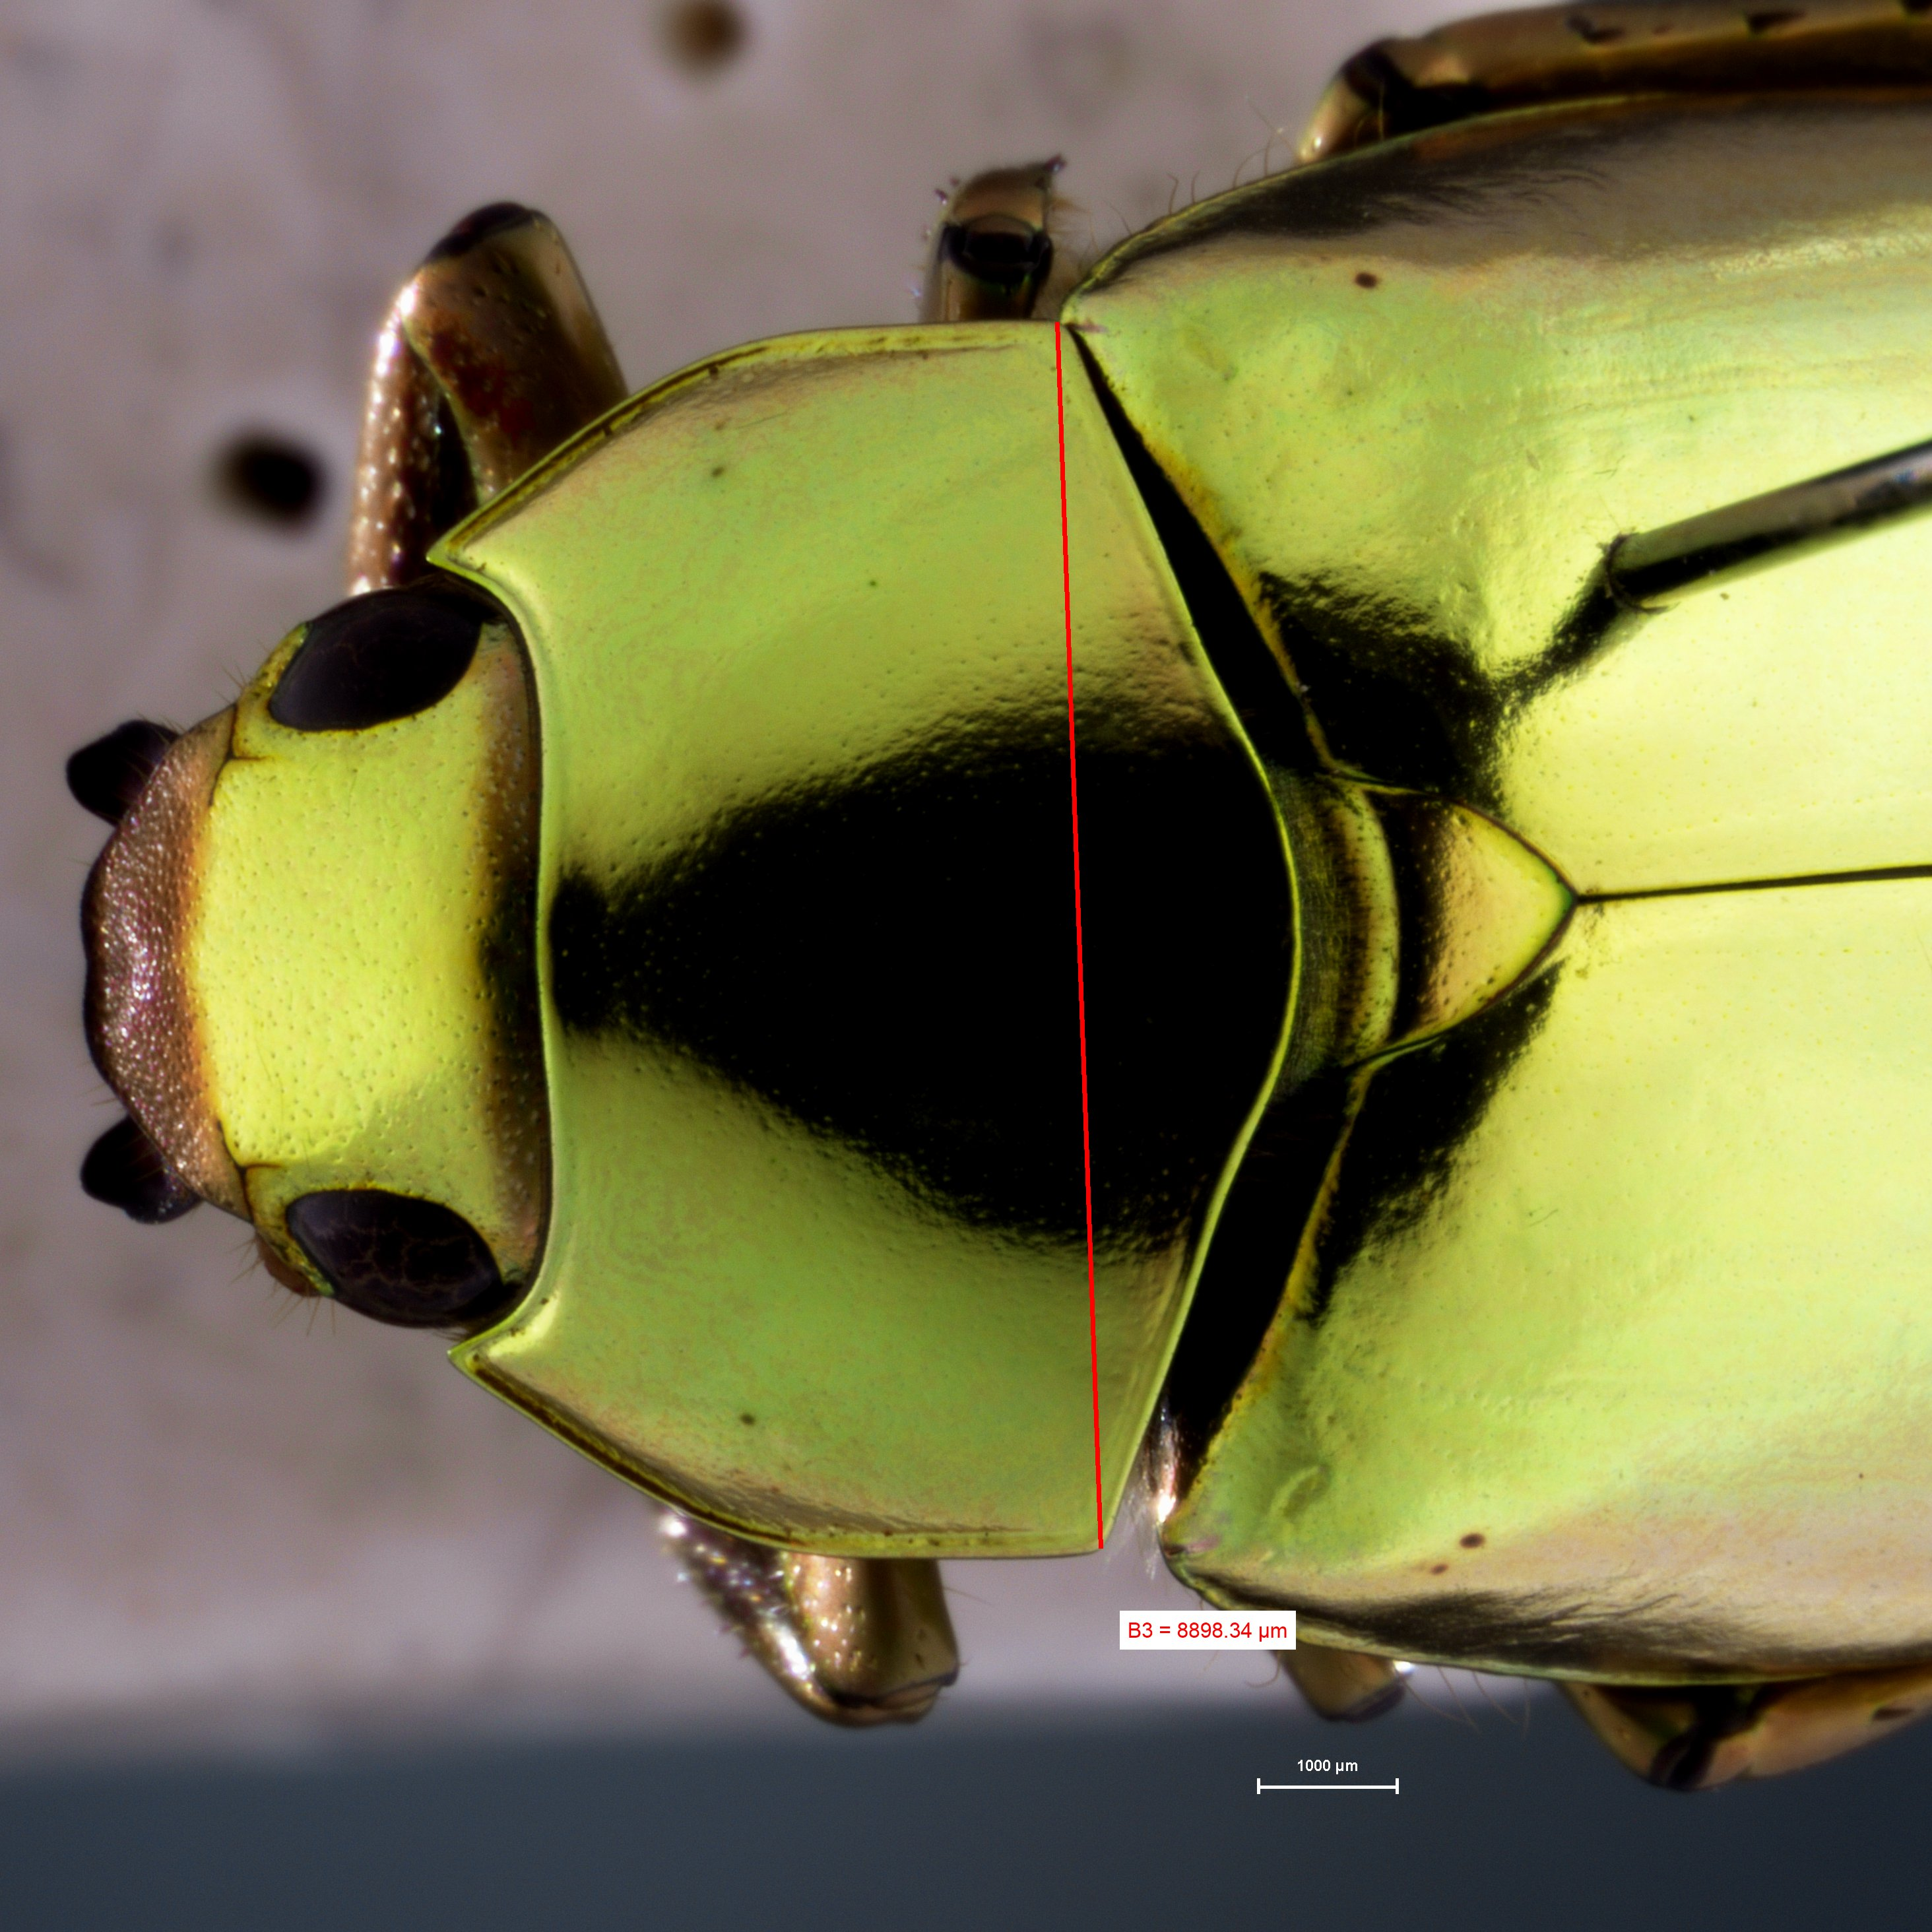
\includegraphics[width=0.5\linewidth]{images/protocol/Pronotum_B3.png}
\caption{ Metric B3}
\end{figure}

\newpage
\subsection*{Metric: B4}

Vertical length of the pronotum’s measured from the middle point of its front down to the middlepoint of its rear

\begin{figure}[H]
\centering
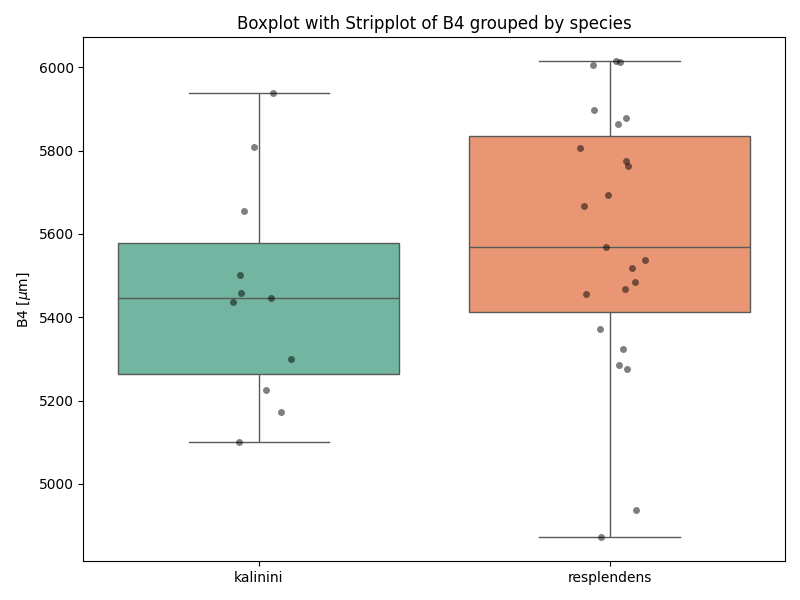
\includegraphics[width=0.7\linewidth]{images/boxplot/boxplot_B4.png}
\caption{  Boxplot and specimen distribution (superposed) for the metric  B4 by species}
\end{figure}

\noindent\textbf{Test Type:} Student's t-test \\
\noindent\textbf{Test Statistic:} -1.155 \\
\noindent\textbf{P-value:} 0.257 \\
\noindent\textbf{Interpretation:} no significant difference

\begin{figure}[H]
\centering
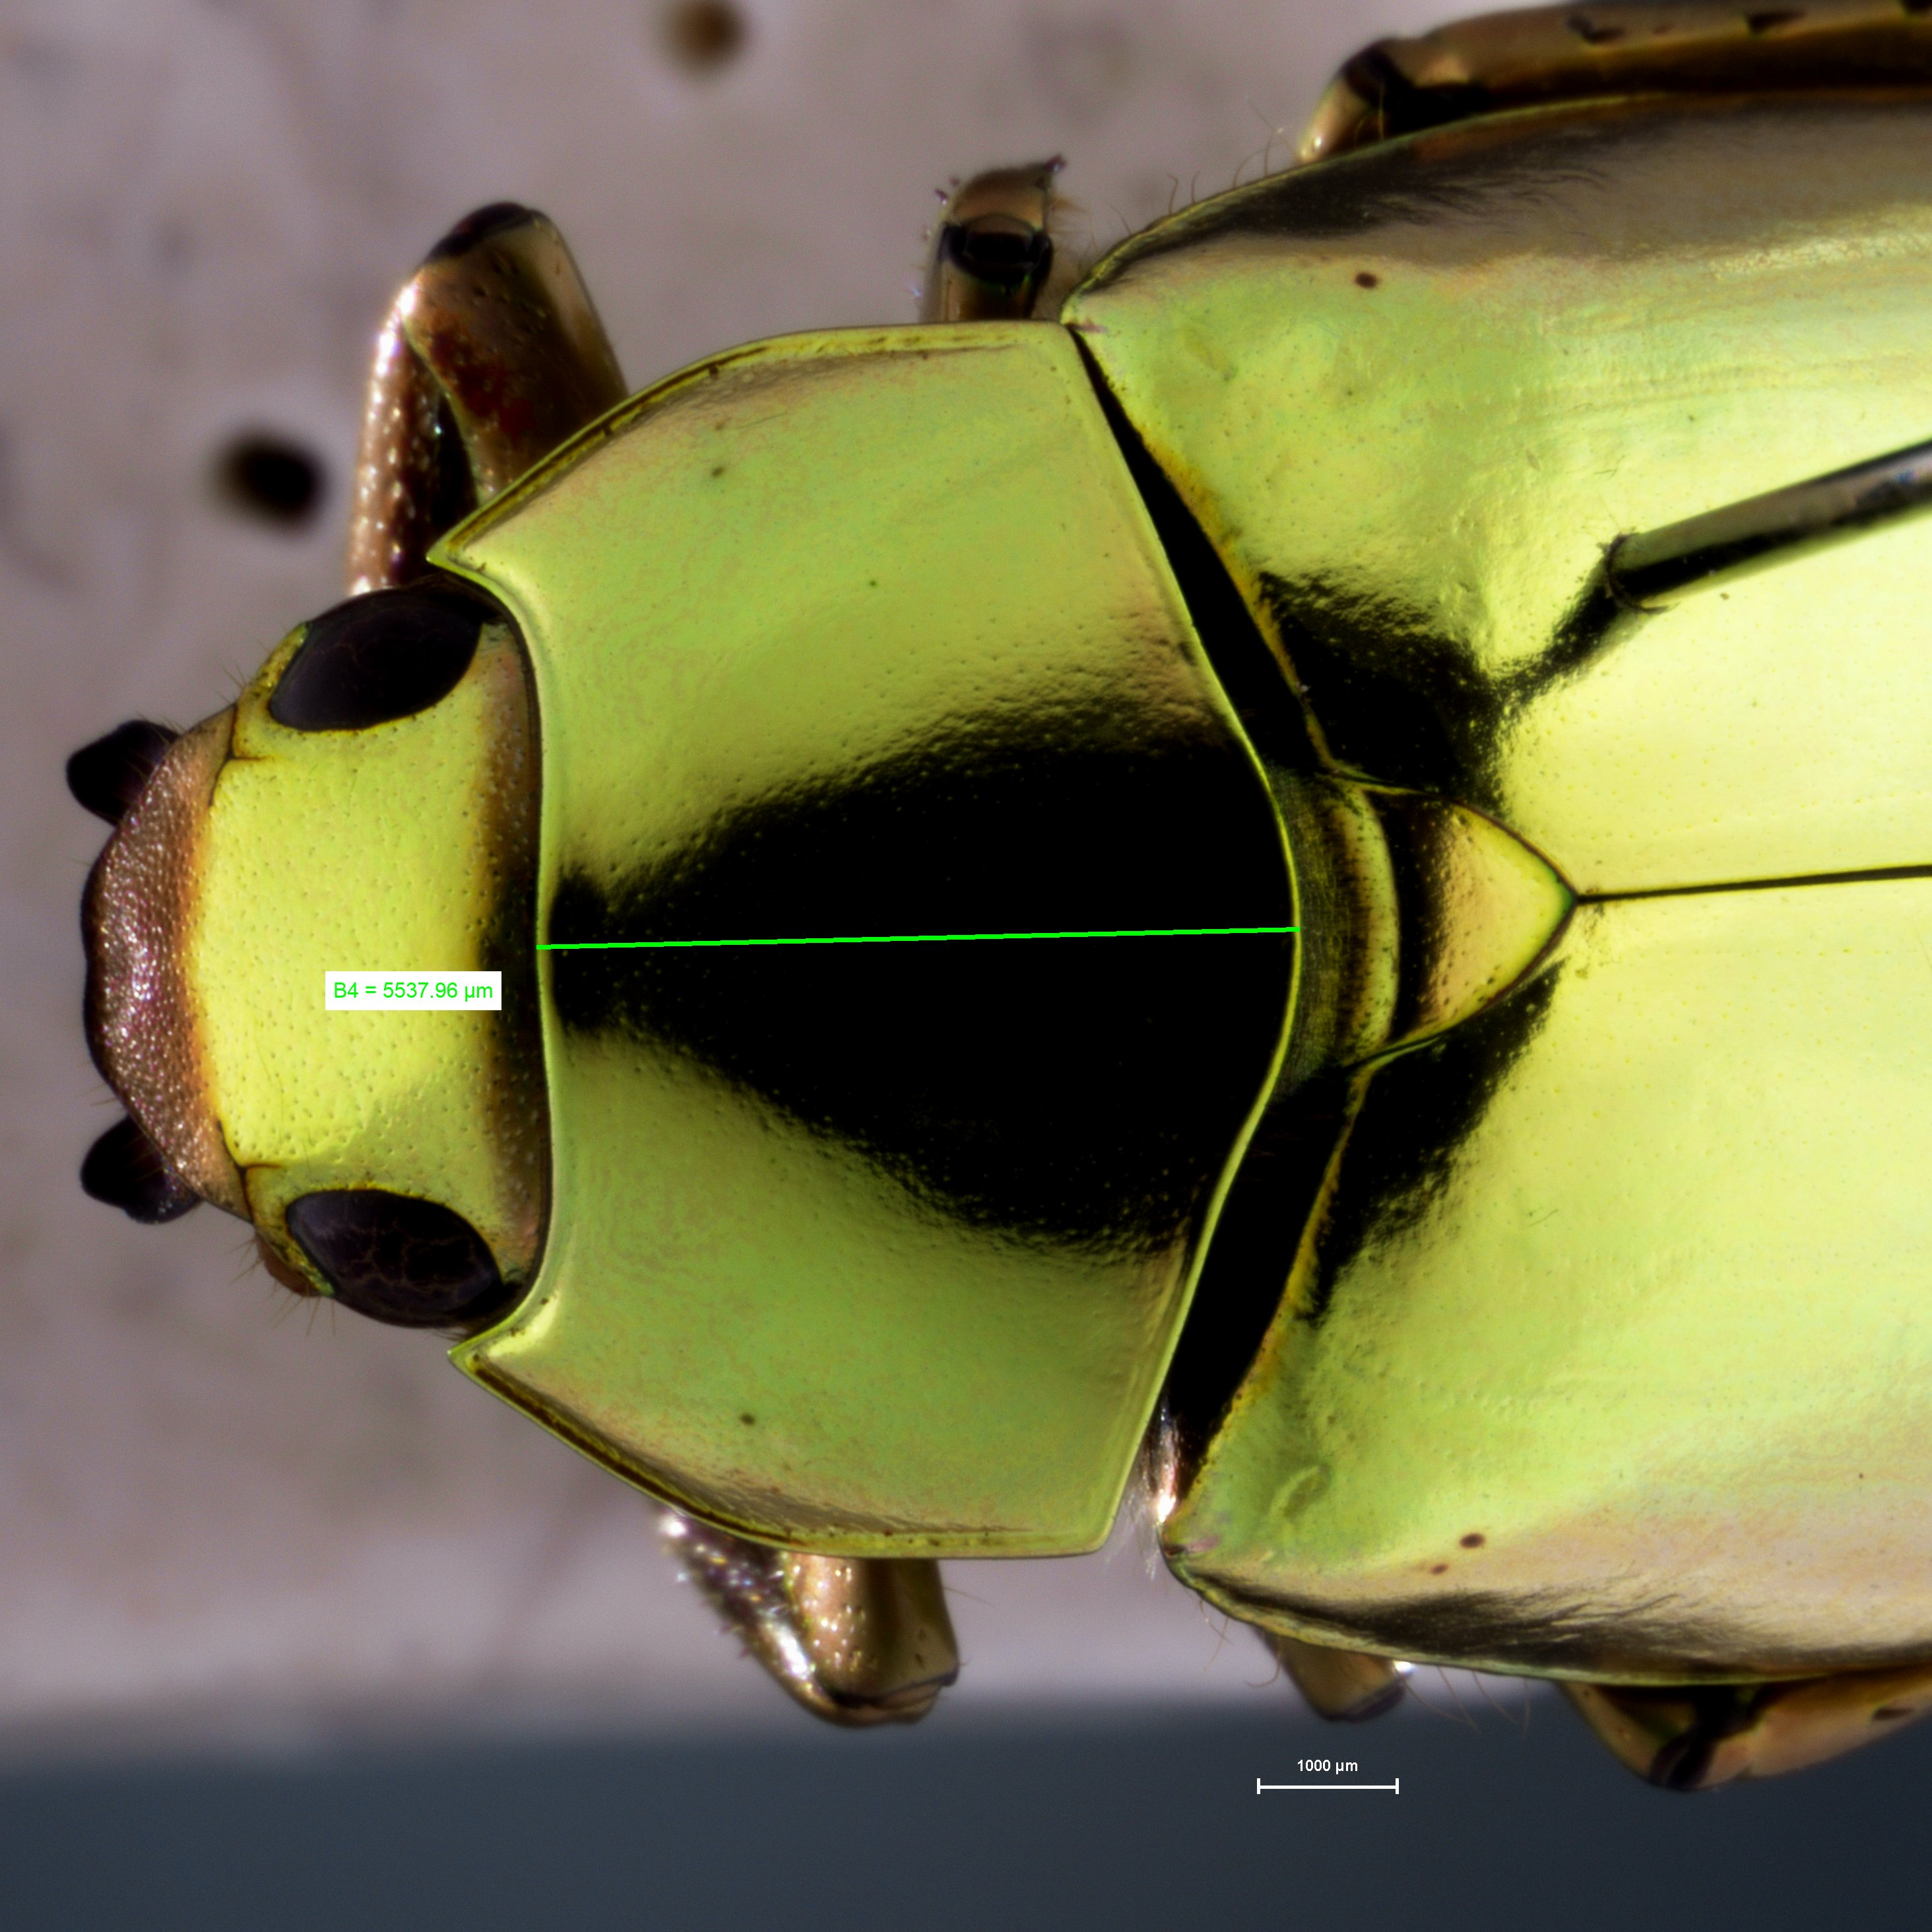
\includegraphics[width=0.5\linewidth]{images/protocol/Pronotum_B4.png}
\caption{ Metric B4}
\end{figure}

\newpage
\subsection*{Metric: B5}

Angle of its side measured between the tangent lines to its straightest sections in the front and back, as seen from the top 

\begin{figure}[H]
\centering
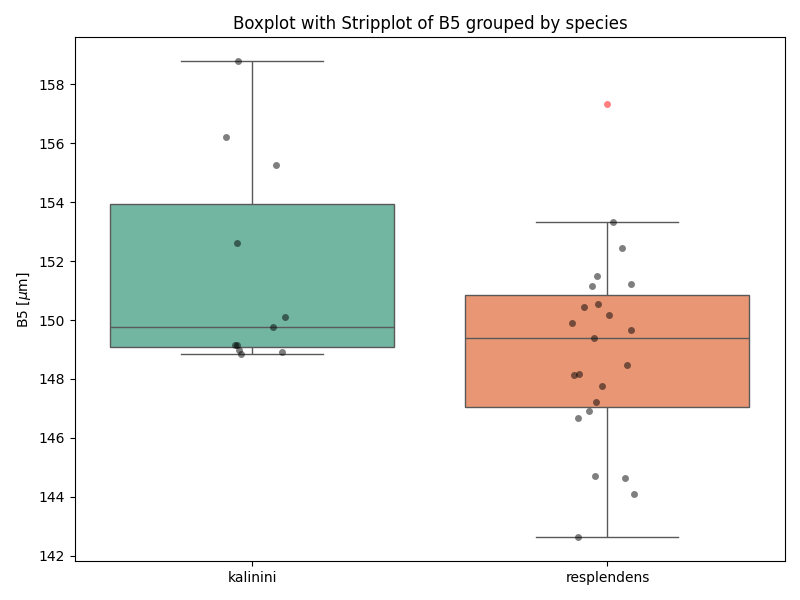
\includegraphics[width=0.7\linewidth]{images/boxplot/boxplot_B5.png}
\caption{  Boxplot and specimen distribution (superposed) for the metric  B5 by species}
\end{figure}

\noindent\textbf{Test Type:} Mann-Whitney U test \\
\noindent\textbf{Test Statistic:} 170.000 \\
\noindent\textbf{P-value:} 0.113 \\
\noindent\textbf{Interpretation:} no significant difference

\begin{figure}[H]
\centering
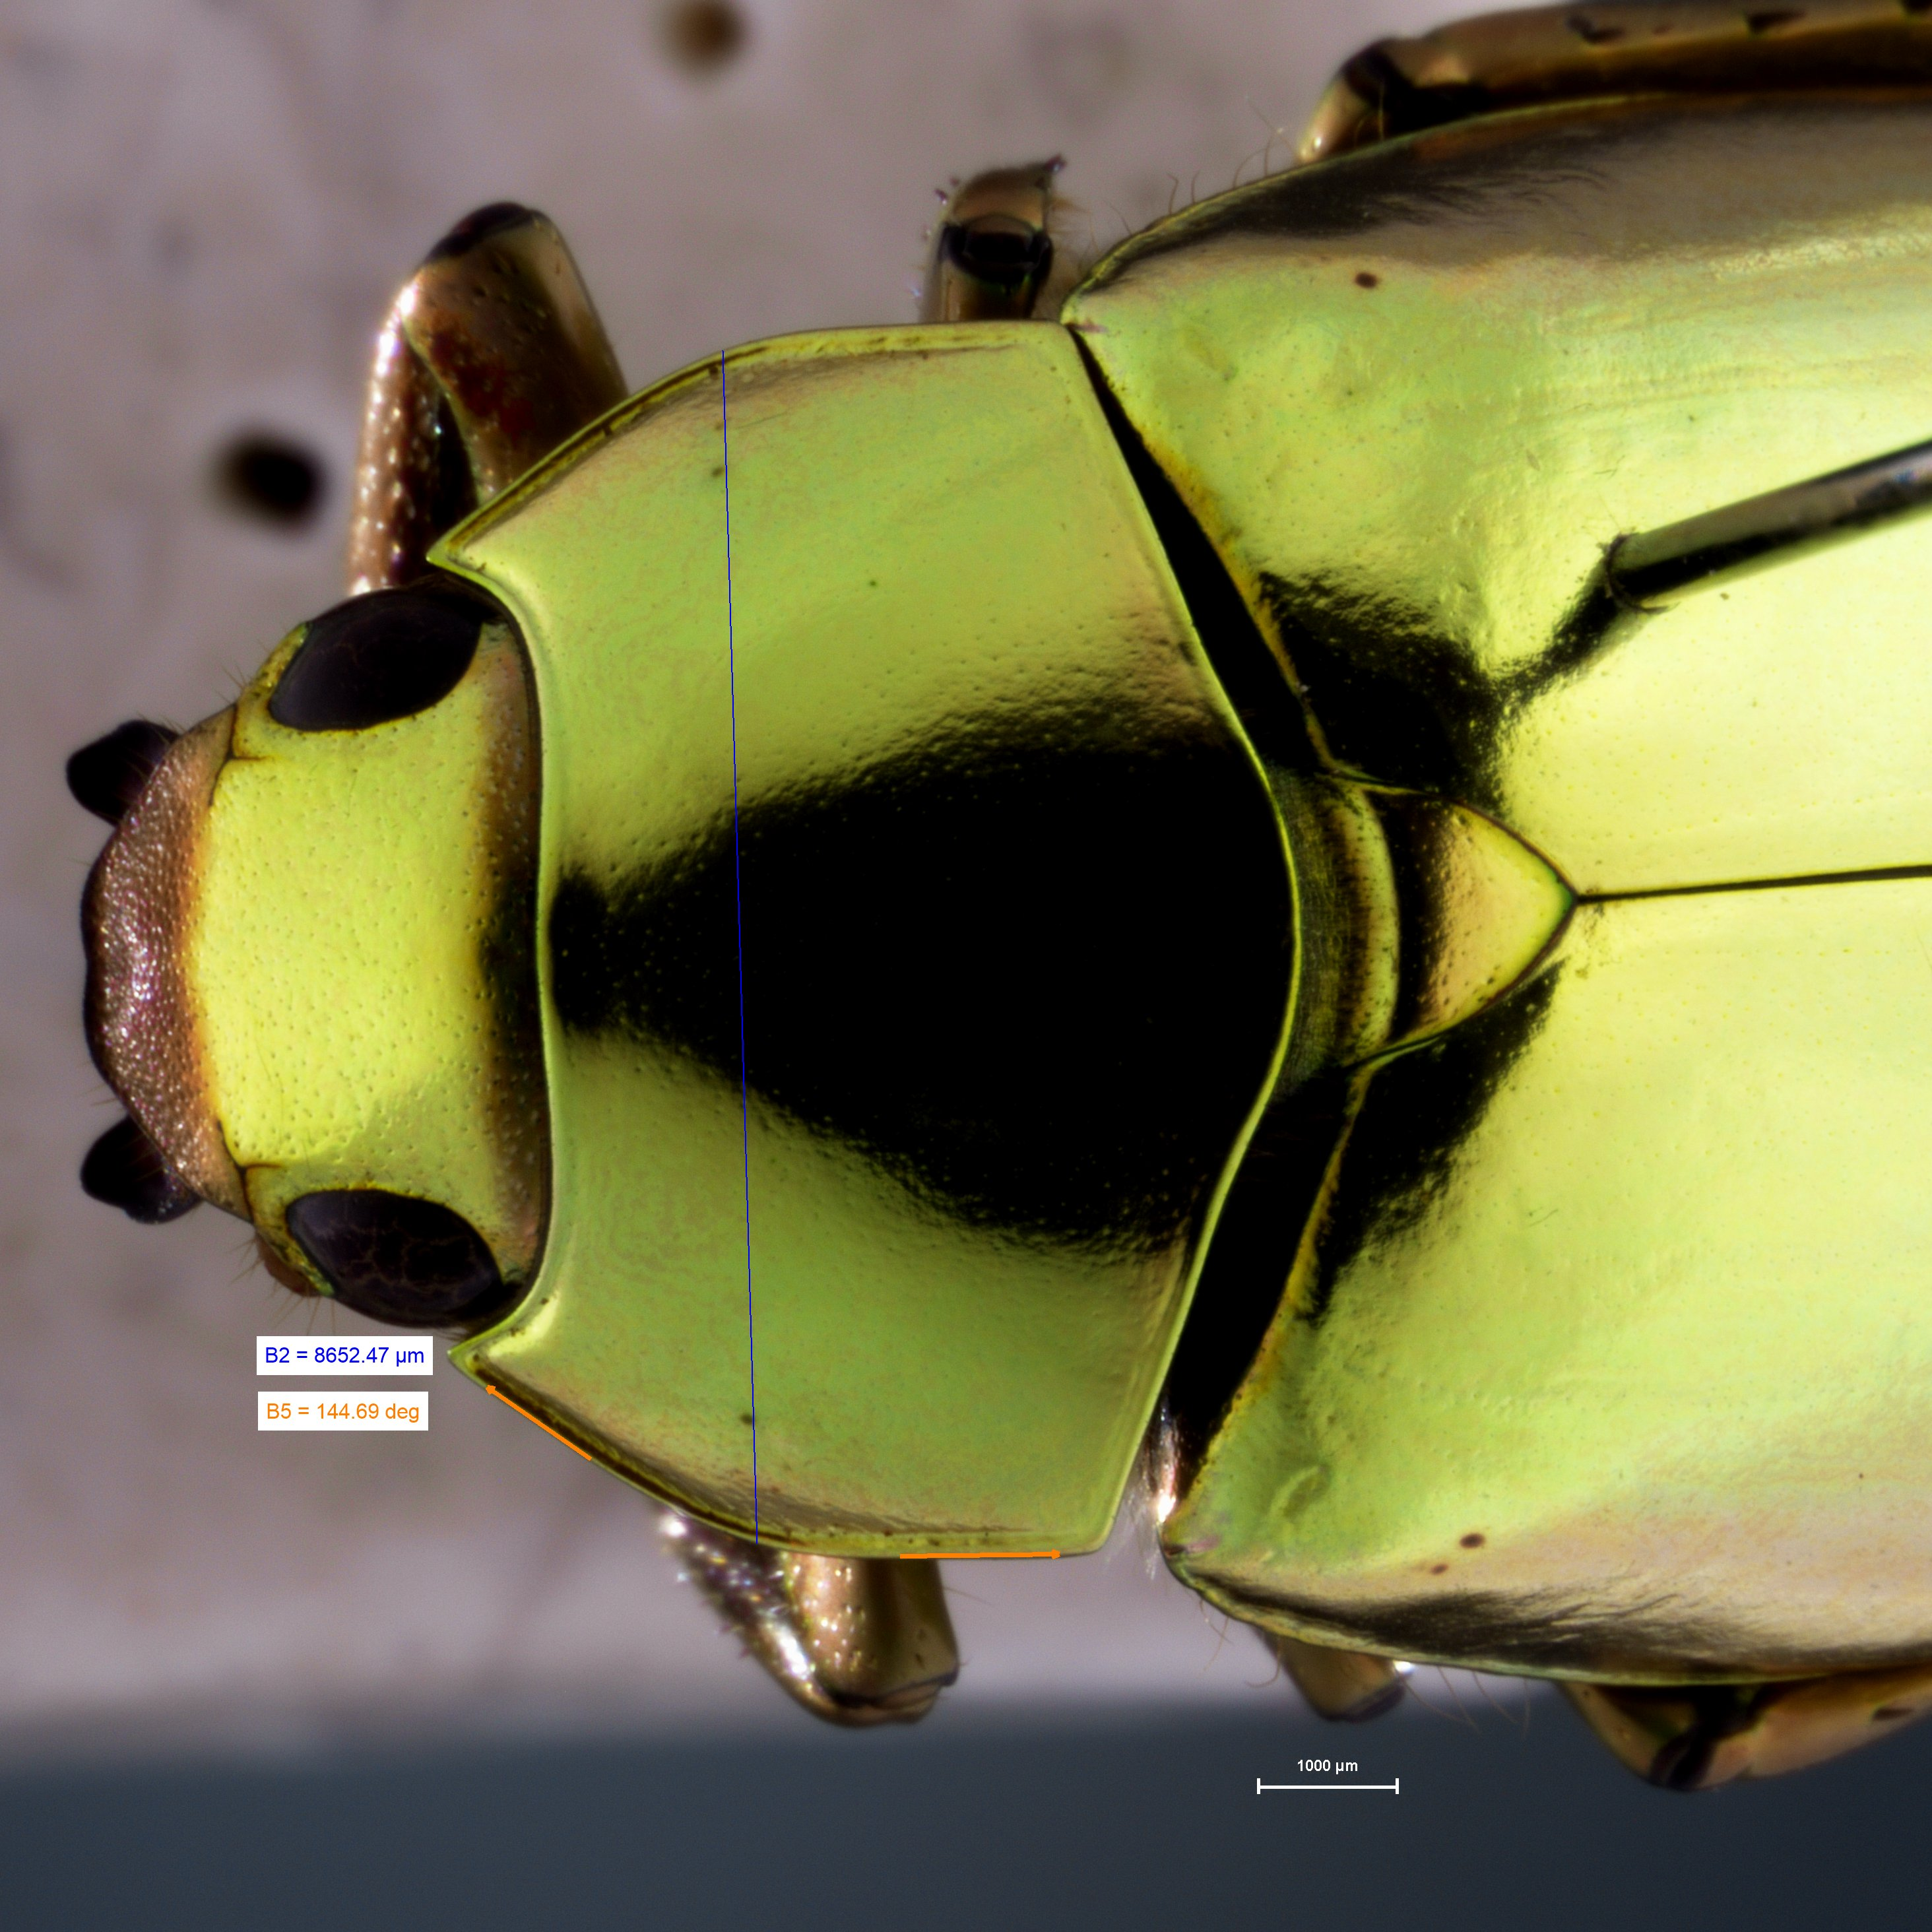
\includegraphics[width=0.5\linewidth]{images/protocol/Pronotum_B5.png}
\caption{ Metric B5}
\end{figure}

\newpage
\subsection*{Metric: C1}

Angle of its side measured between the tangent lines to its straightest sections in the front and back as seen by the side

\begin{figure}[H]
\centering
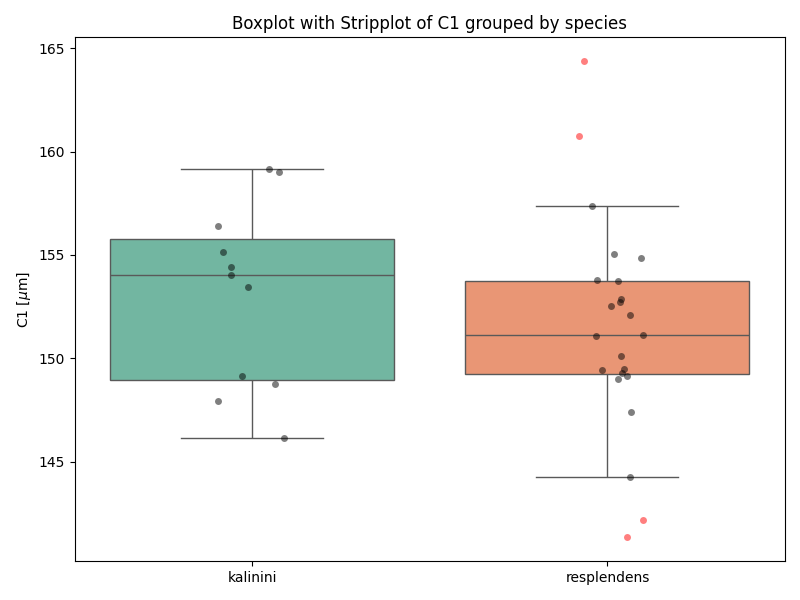
\includegraphics[width=0.7\linewidth]{images/boxplot/boxplot_C1.png}
\caption{  Boxplot and specimen distribution (superposed) for the metric  C1 by species}
\end{figure}

\noindent\textbf{Test Type:} Student's t-test \\
\noindent\textbf{Test Statistic:} 0.851 \\
\noindent\textbf{P-value:} 0.401 \\
\noindent\textbf{Interpretation:} no significant difference

\begin{figure}[H]
\centering
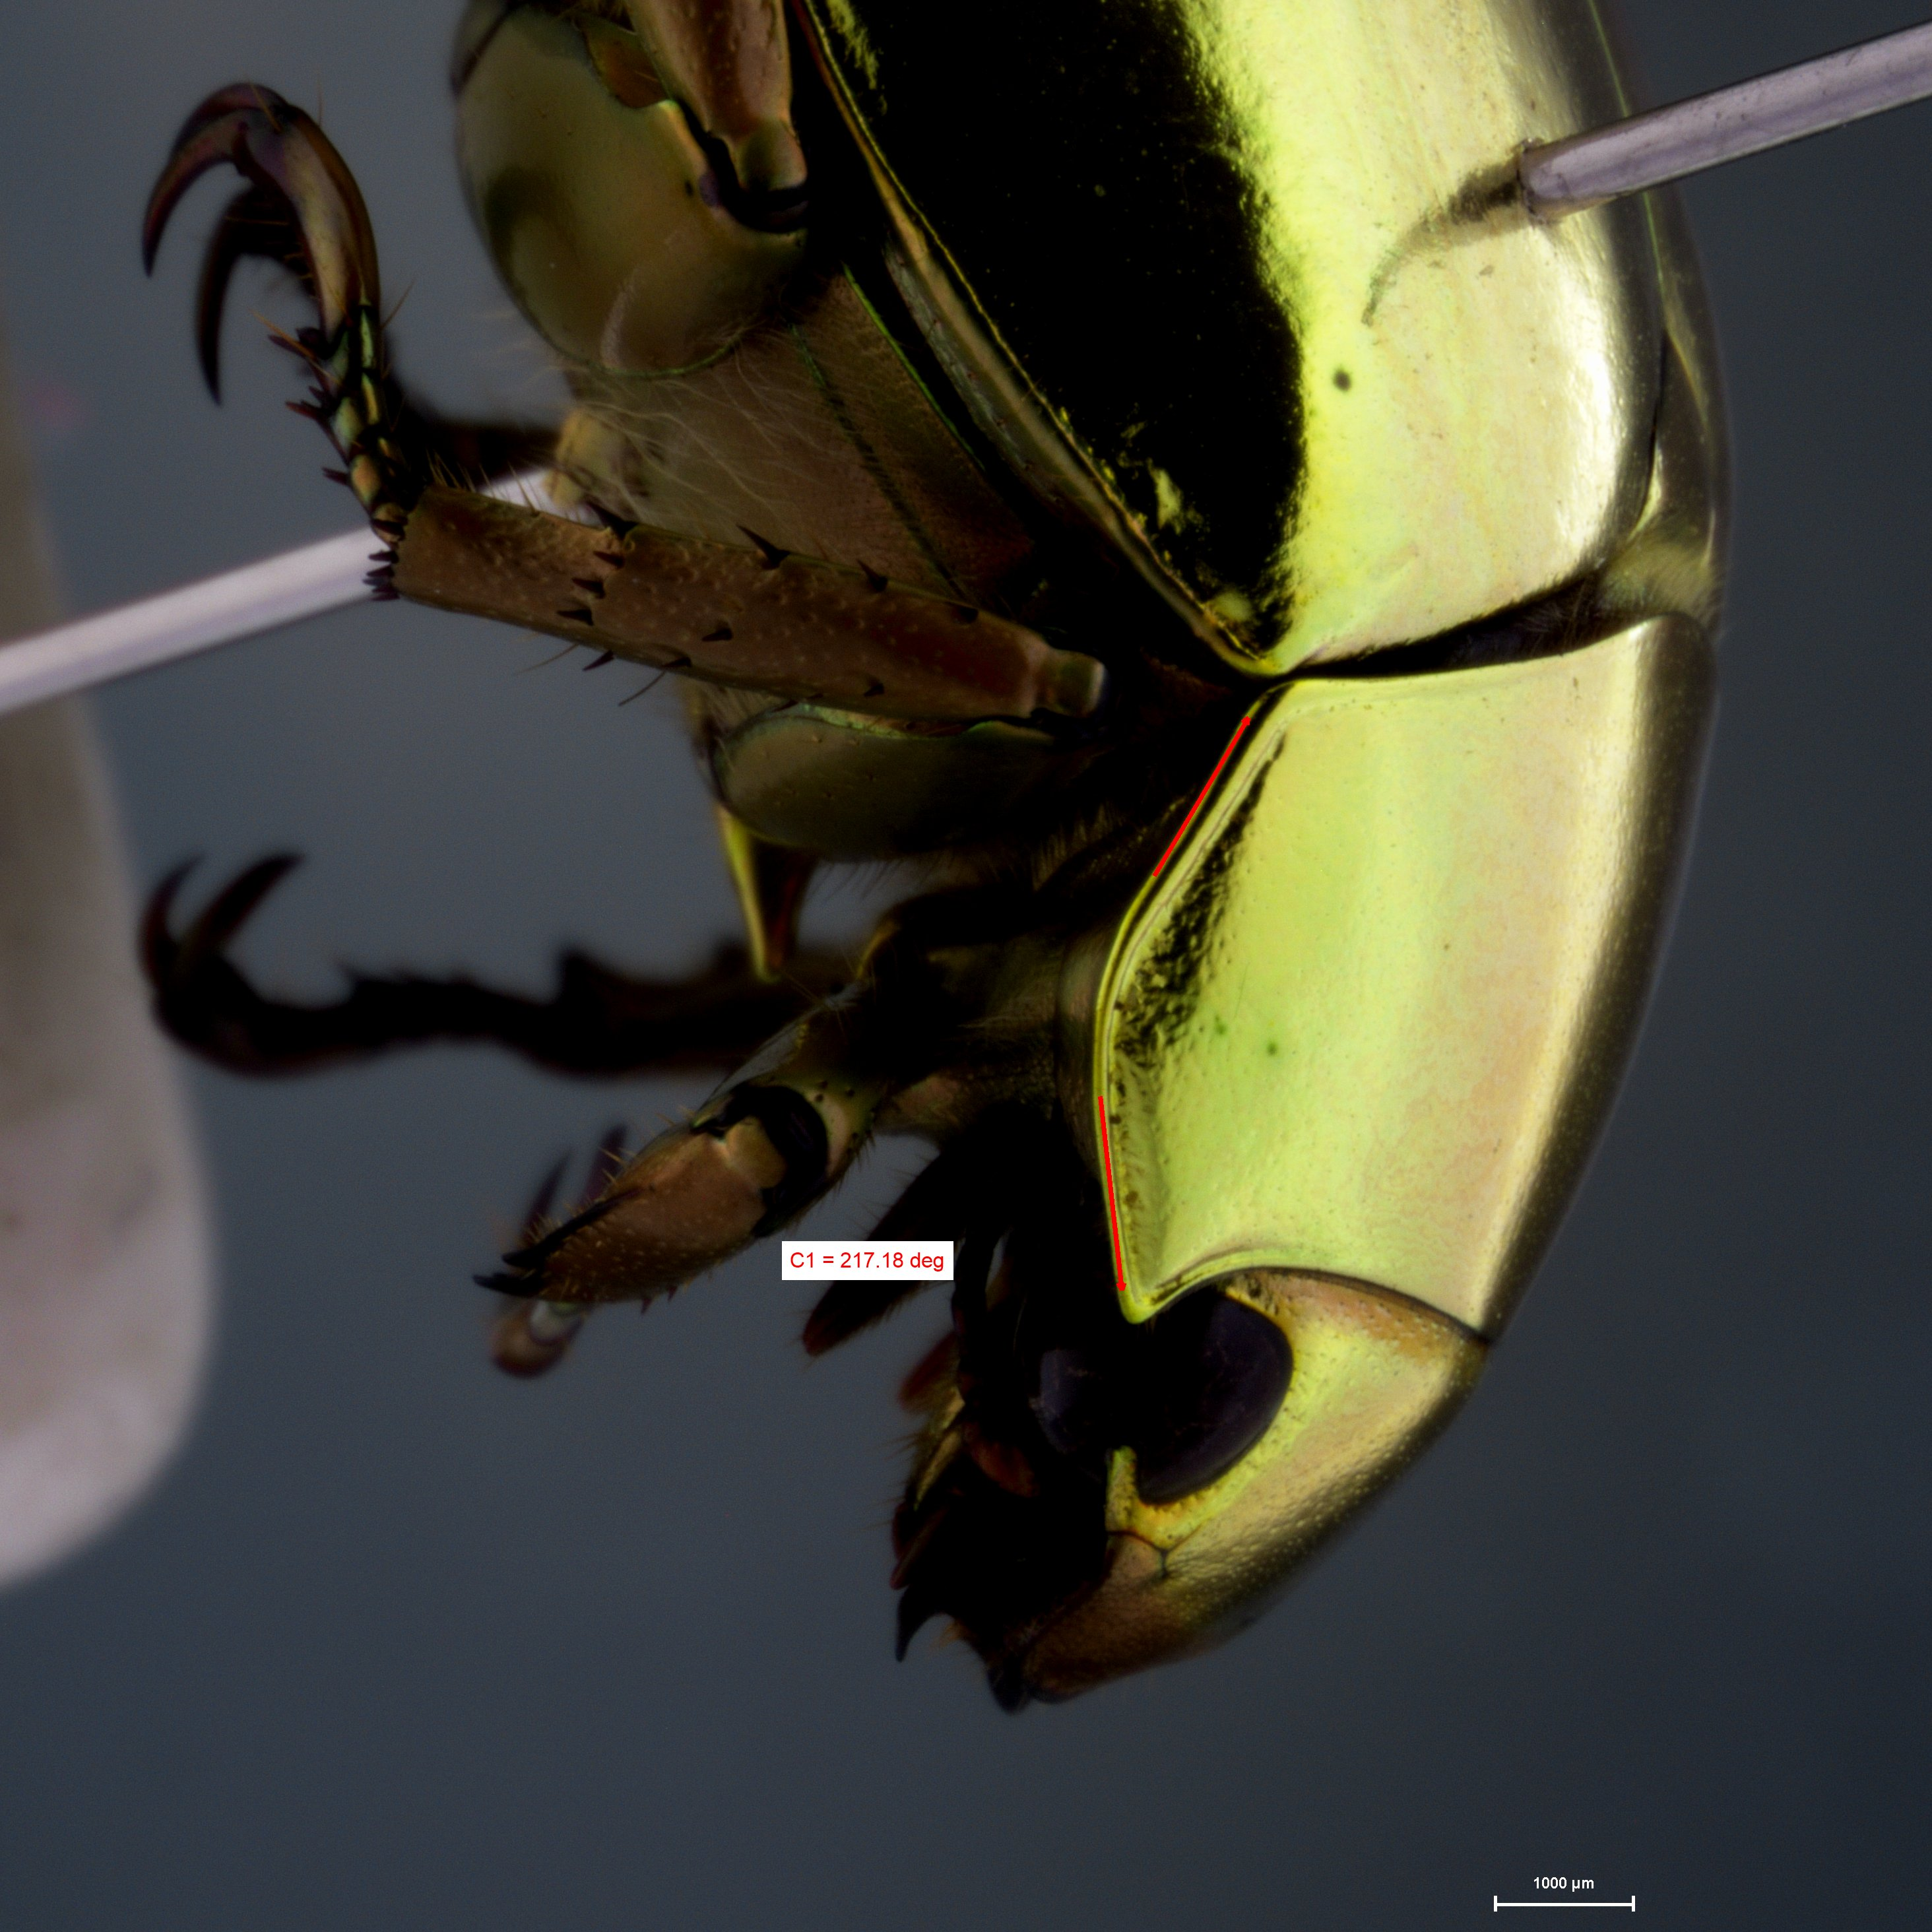
\includegraphics[width=0.5\linewidth]{images/protocol/Lateral_C1.png}
\caption{ Metric C1}
\end{figure}

\newpage
\subsection*{Metric: D1}

Mesosternal process’ horizontal length measured from the secant point of the tangents of its sides with the horizontal line used to measure D1. 

\begin{figure}[H]
\centering
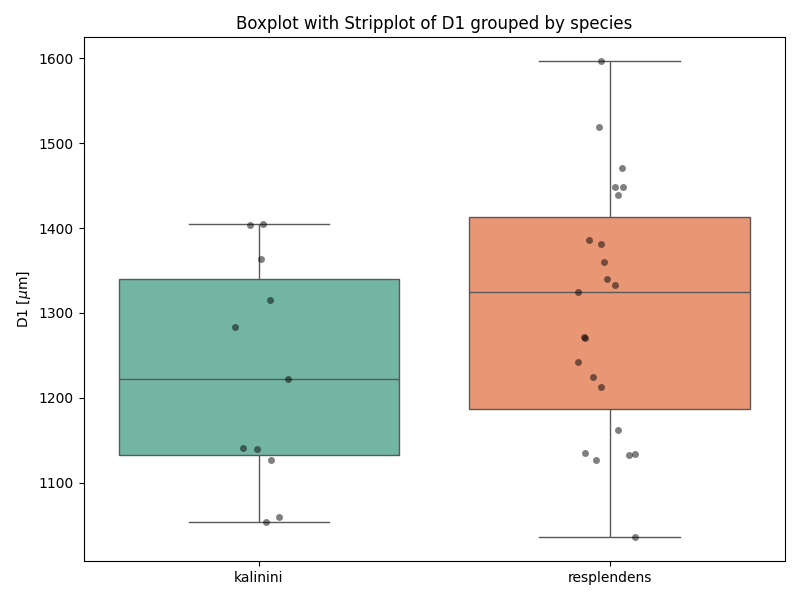
\includegraphics[width=0.7\linewidth]{images/boxplot/boxplot_D1.png}
\caption{  Boxplot and specimen distribution (superposed) for the metric  D1 by species}
\end{figure}

\noindent\textbf{Test Type:} Student's t-test \\
\noindent\textbf{Test Statistic:} -1.458 \\
\noindent\textbf{P-value:} 0.155 \\
\noindent\textbf{Interpretation:} no significant difference

\begin{figure}[H]
\centering
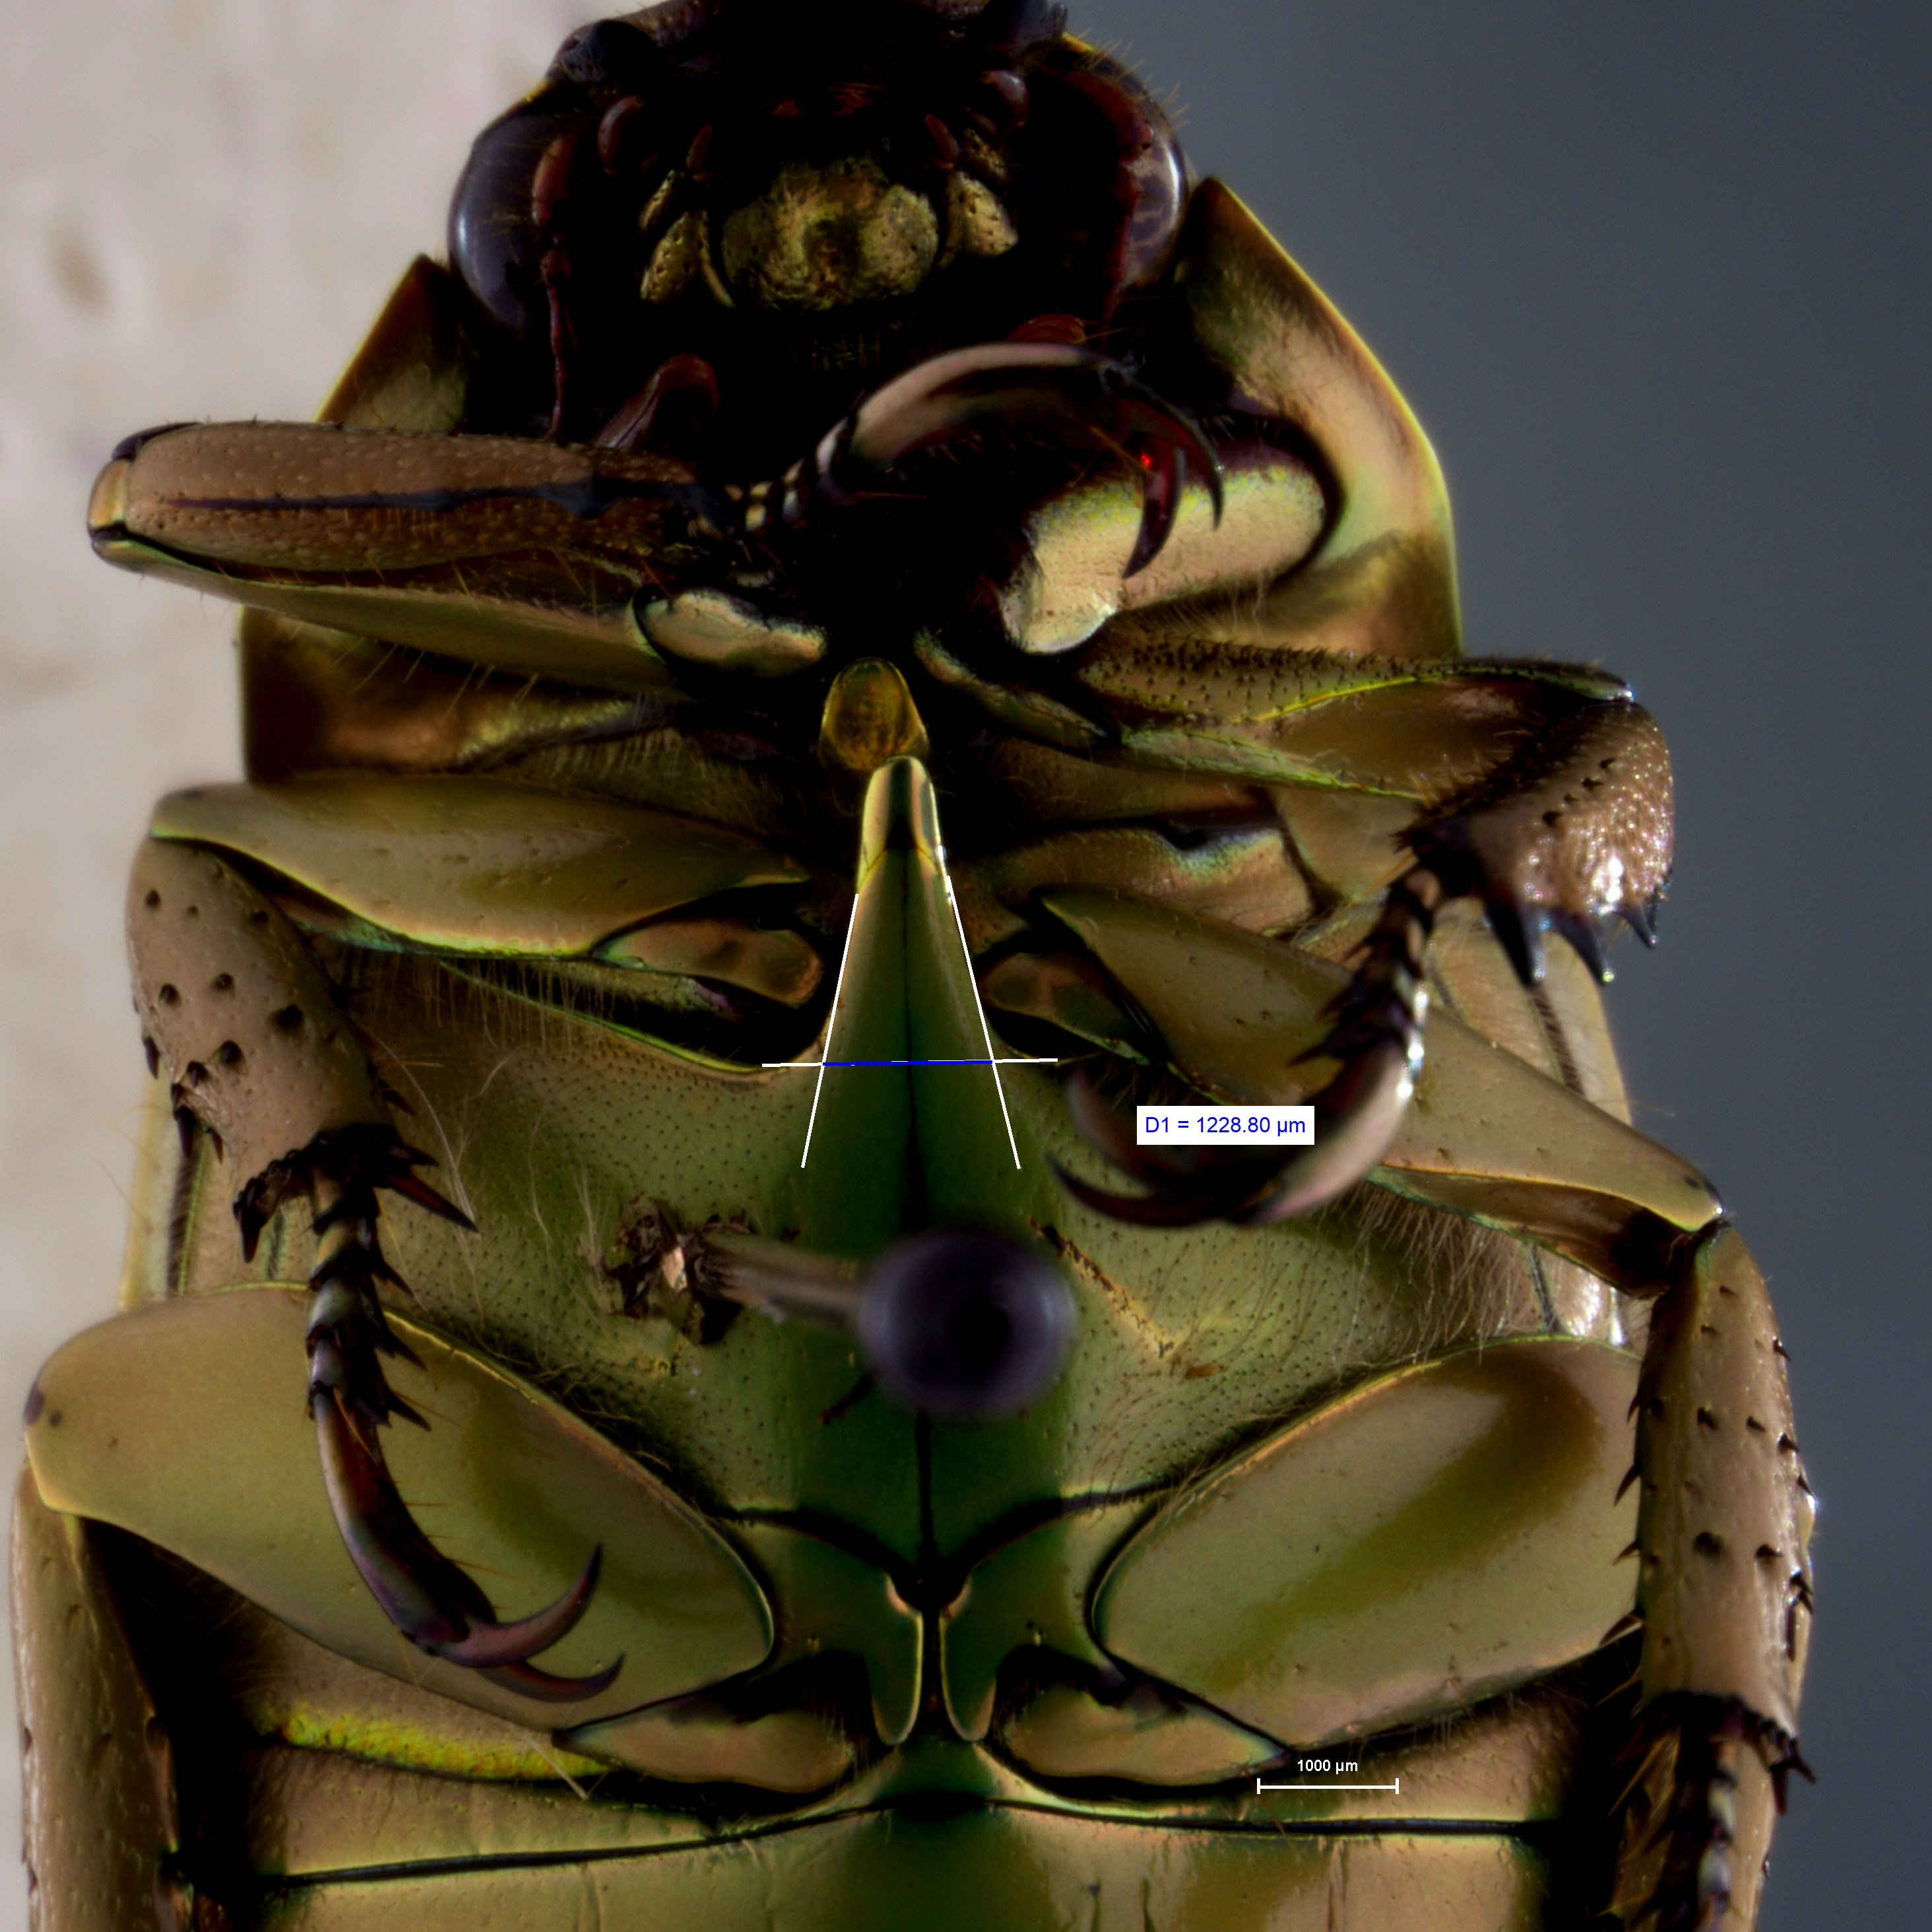
\includegraphics[width=0.5\linewidth]{images/protocol/Mesosternal_process_D1.png}
\caption{ Metric D1}
\end{figure}

\newpage
\subsection*{Metric: D2}

Mesosternal process’ vertical length measured from the tip of the mesosternal process down to the line that joins the two lowest curves at the sides of the mesosternal process base

\begin{figure}[H]
\centering
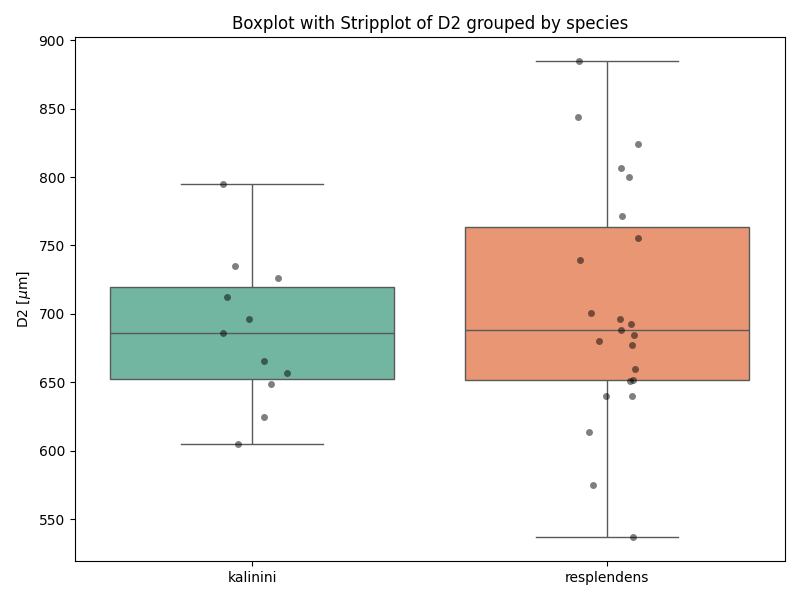
\includegraphics[width=0.7\linewidth]{images/boxplot/boxplot_D2.png}
\caption{  Boxplot and specimen distribution (superposed) for the metric  D2 by species}
\end{figure}

\noindent\textbf{Test Type:} Student's t-test \\
\noindent\textbf{Test Statistic:} -0.647 \\
\noindent\textbf{P-value:} 0.522 \\
\noindent\textbf{Interpretation:} no significant difference

\begin{figure}[H]
\centering
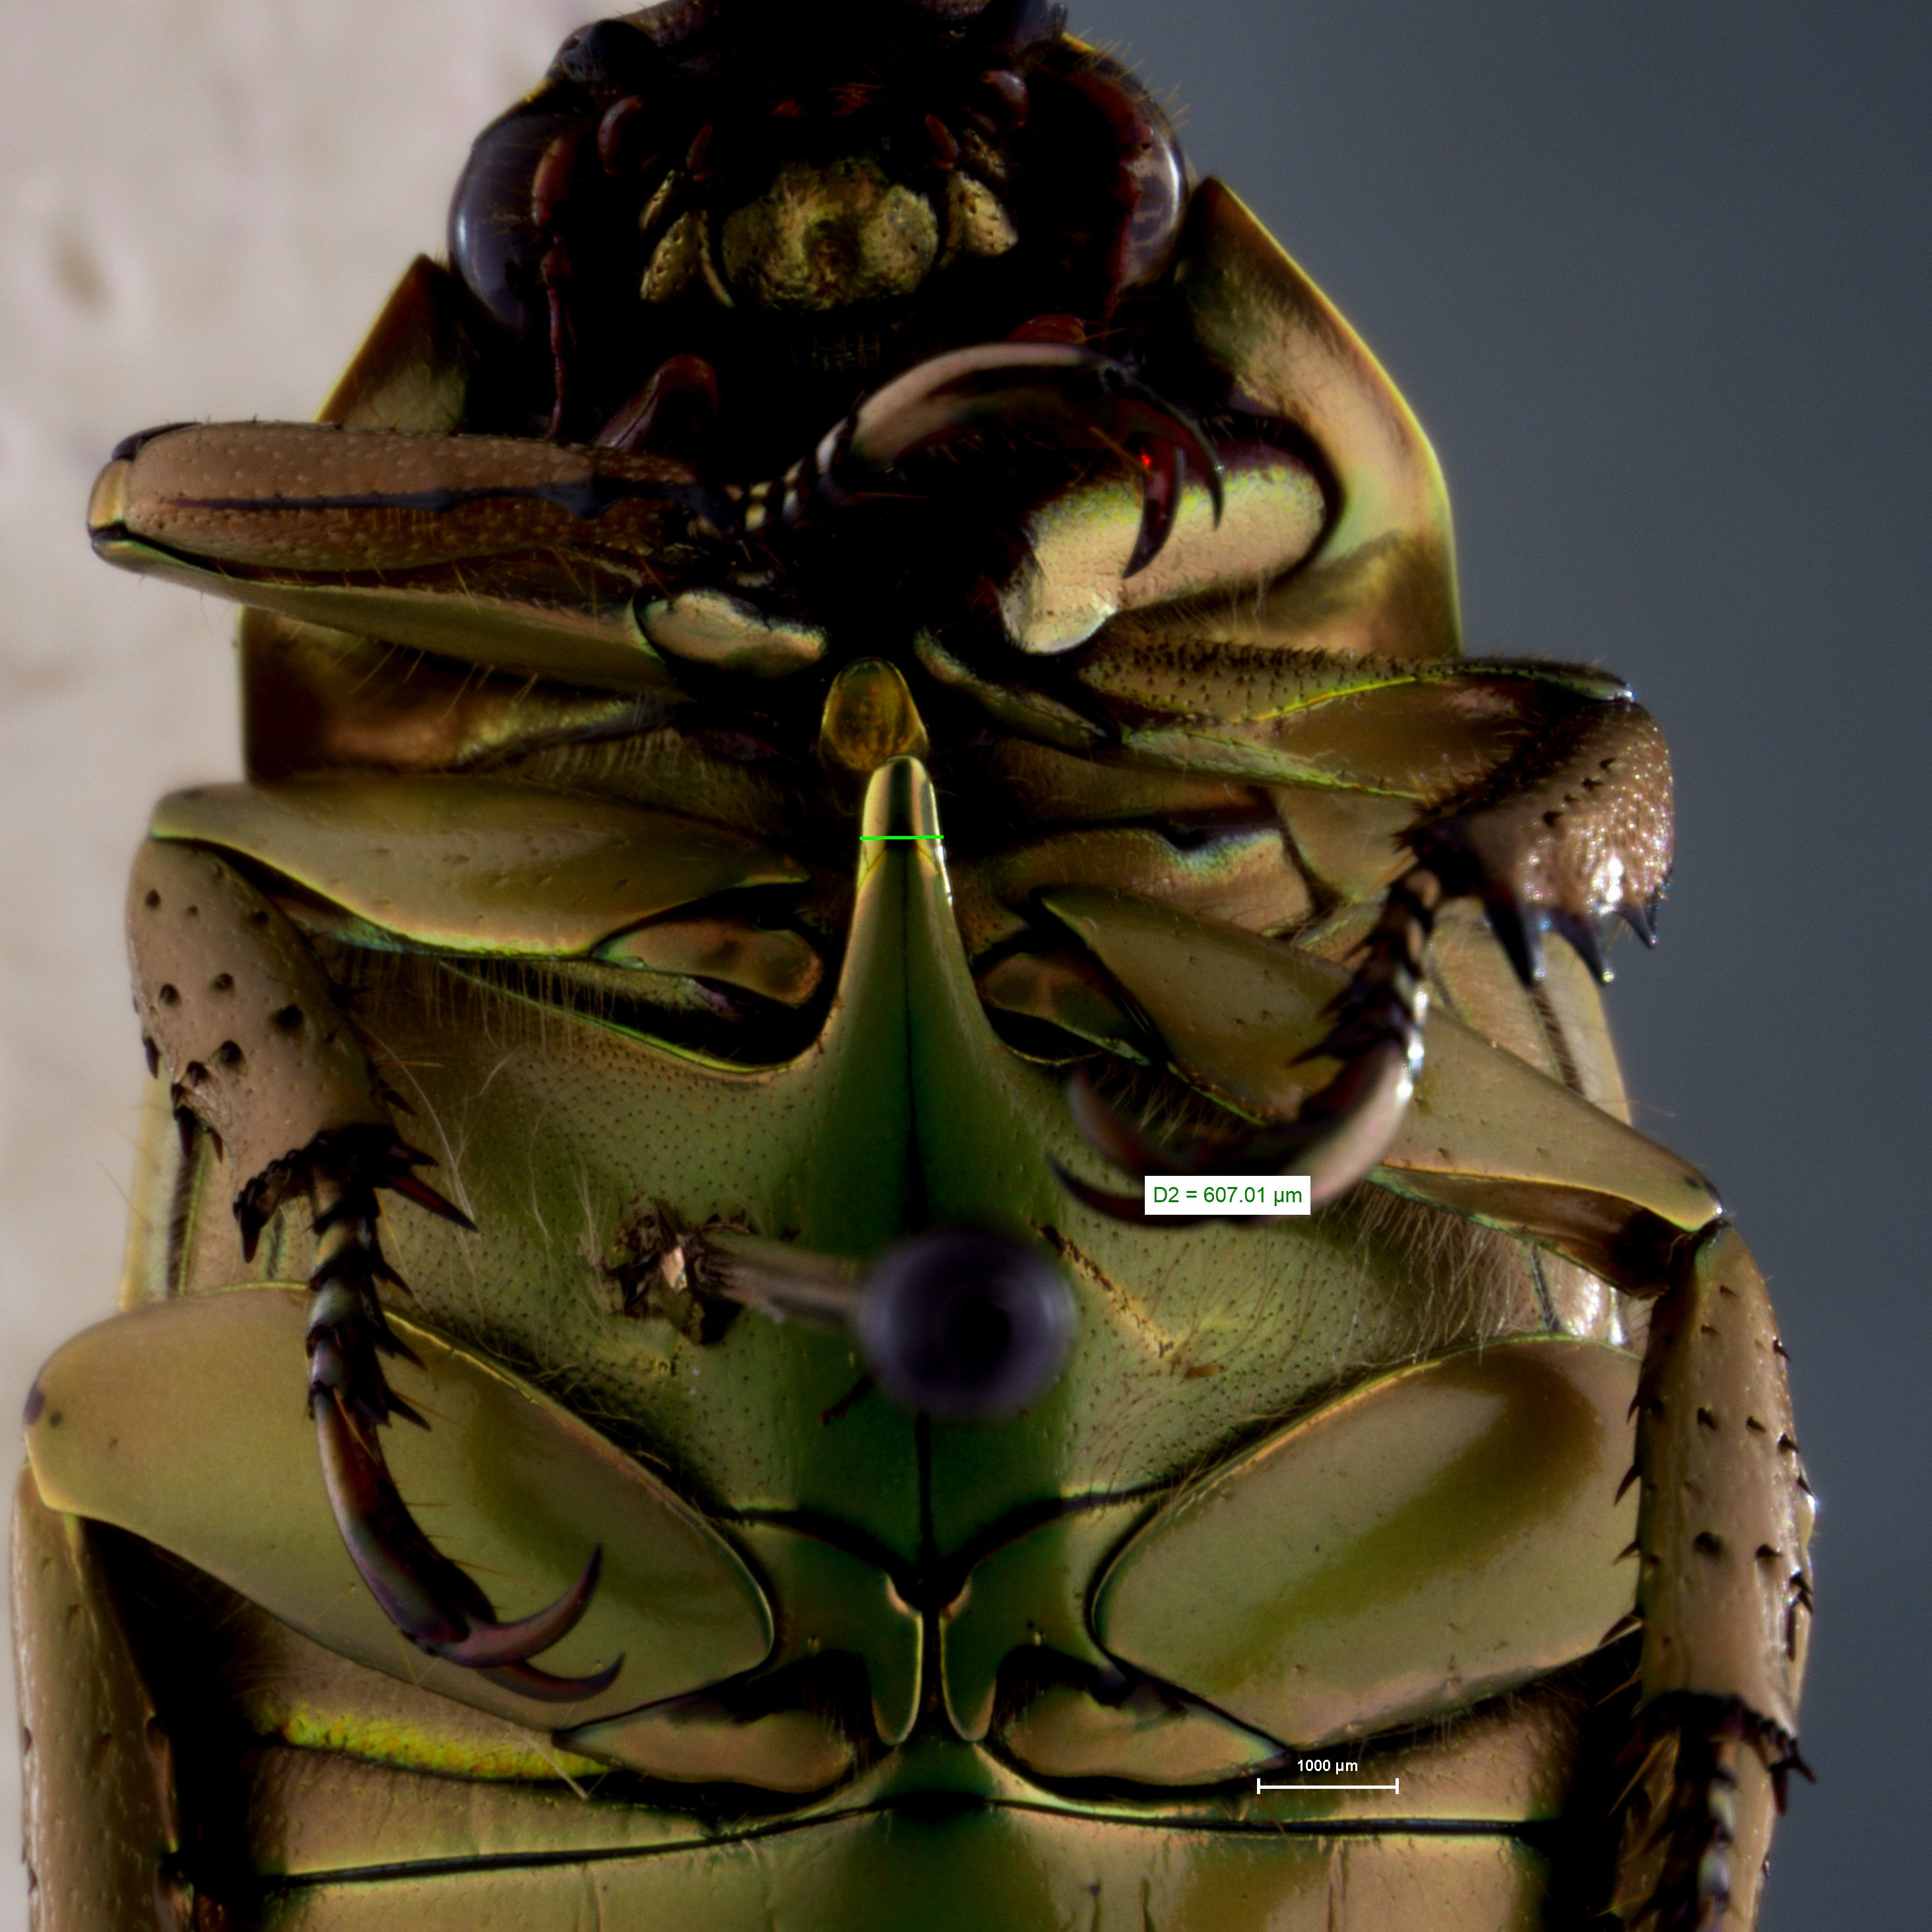
\includegraphics[width=0.5\linewidth]{images/protocol/Mesosternal_process_D2.png}
\caption{ Metric D2}
\end{figure}

\newpage
\subsection*{Metric: D3}

Horizontal width of the dark middle line measured from its two lower ends

\begin{figure}[H]
\centering
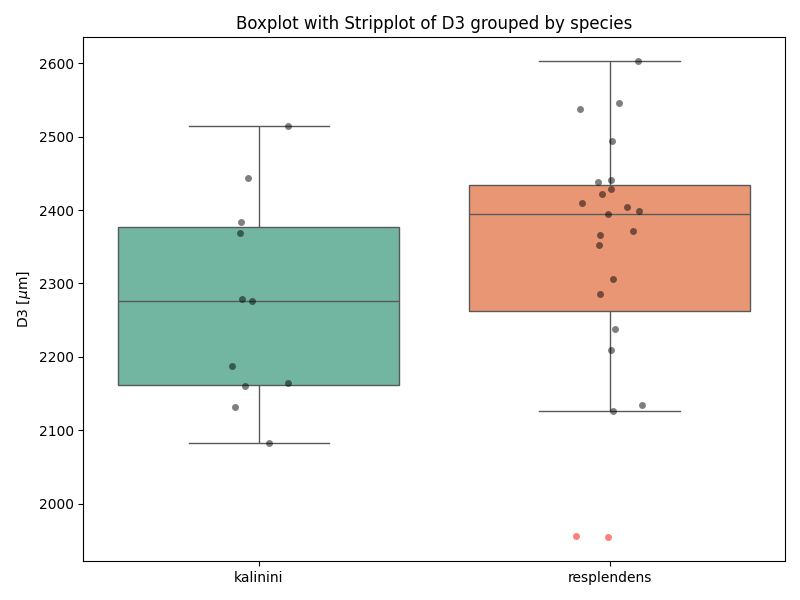
\includegraphics[width=0.7\linewidth]{images/boxplot/boxplot_D3.png}
\caption{  Boxplot and specimen distribution (superposed) for the metric  D3 by species}
\end{figure}

\noindent\textbf{Test Type:} Student's t-test \\
\noindent\textbf{Test Statistic:} -1.148 \\
\noindent\textbf{P-value:} 0.260 \\
\noindent\textbf{Interpretation:} no significant difference

\begin{figure}[H]
\centering
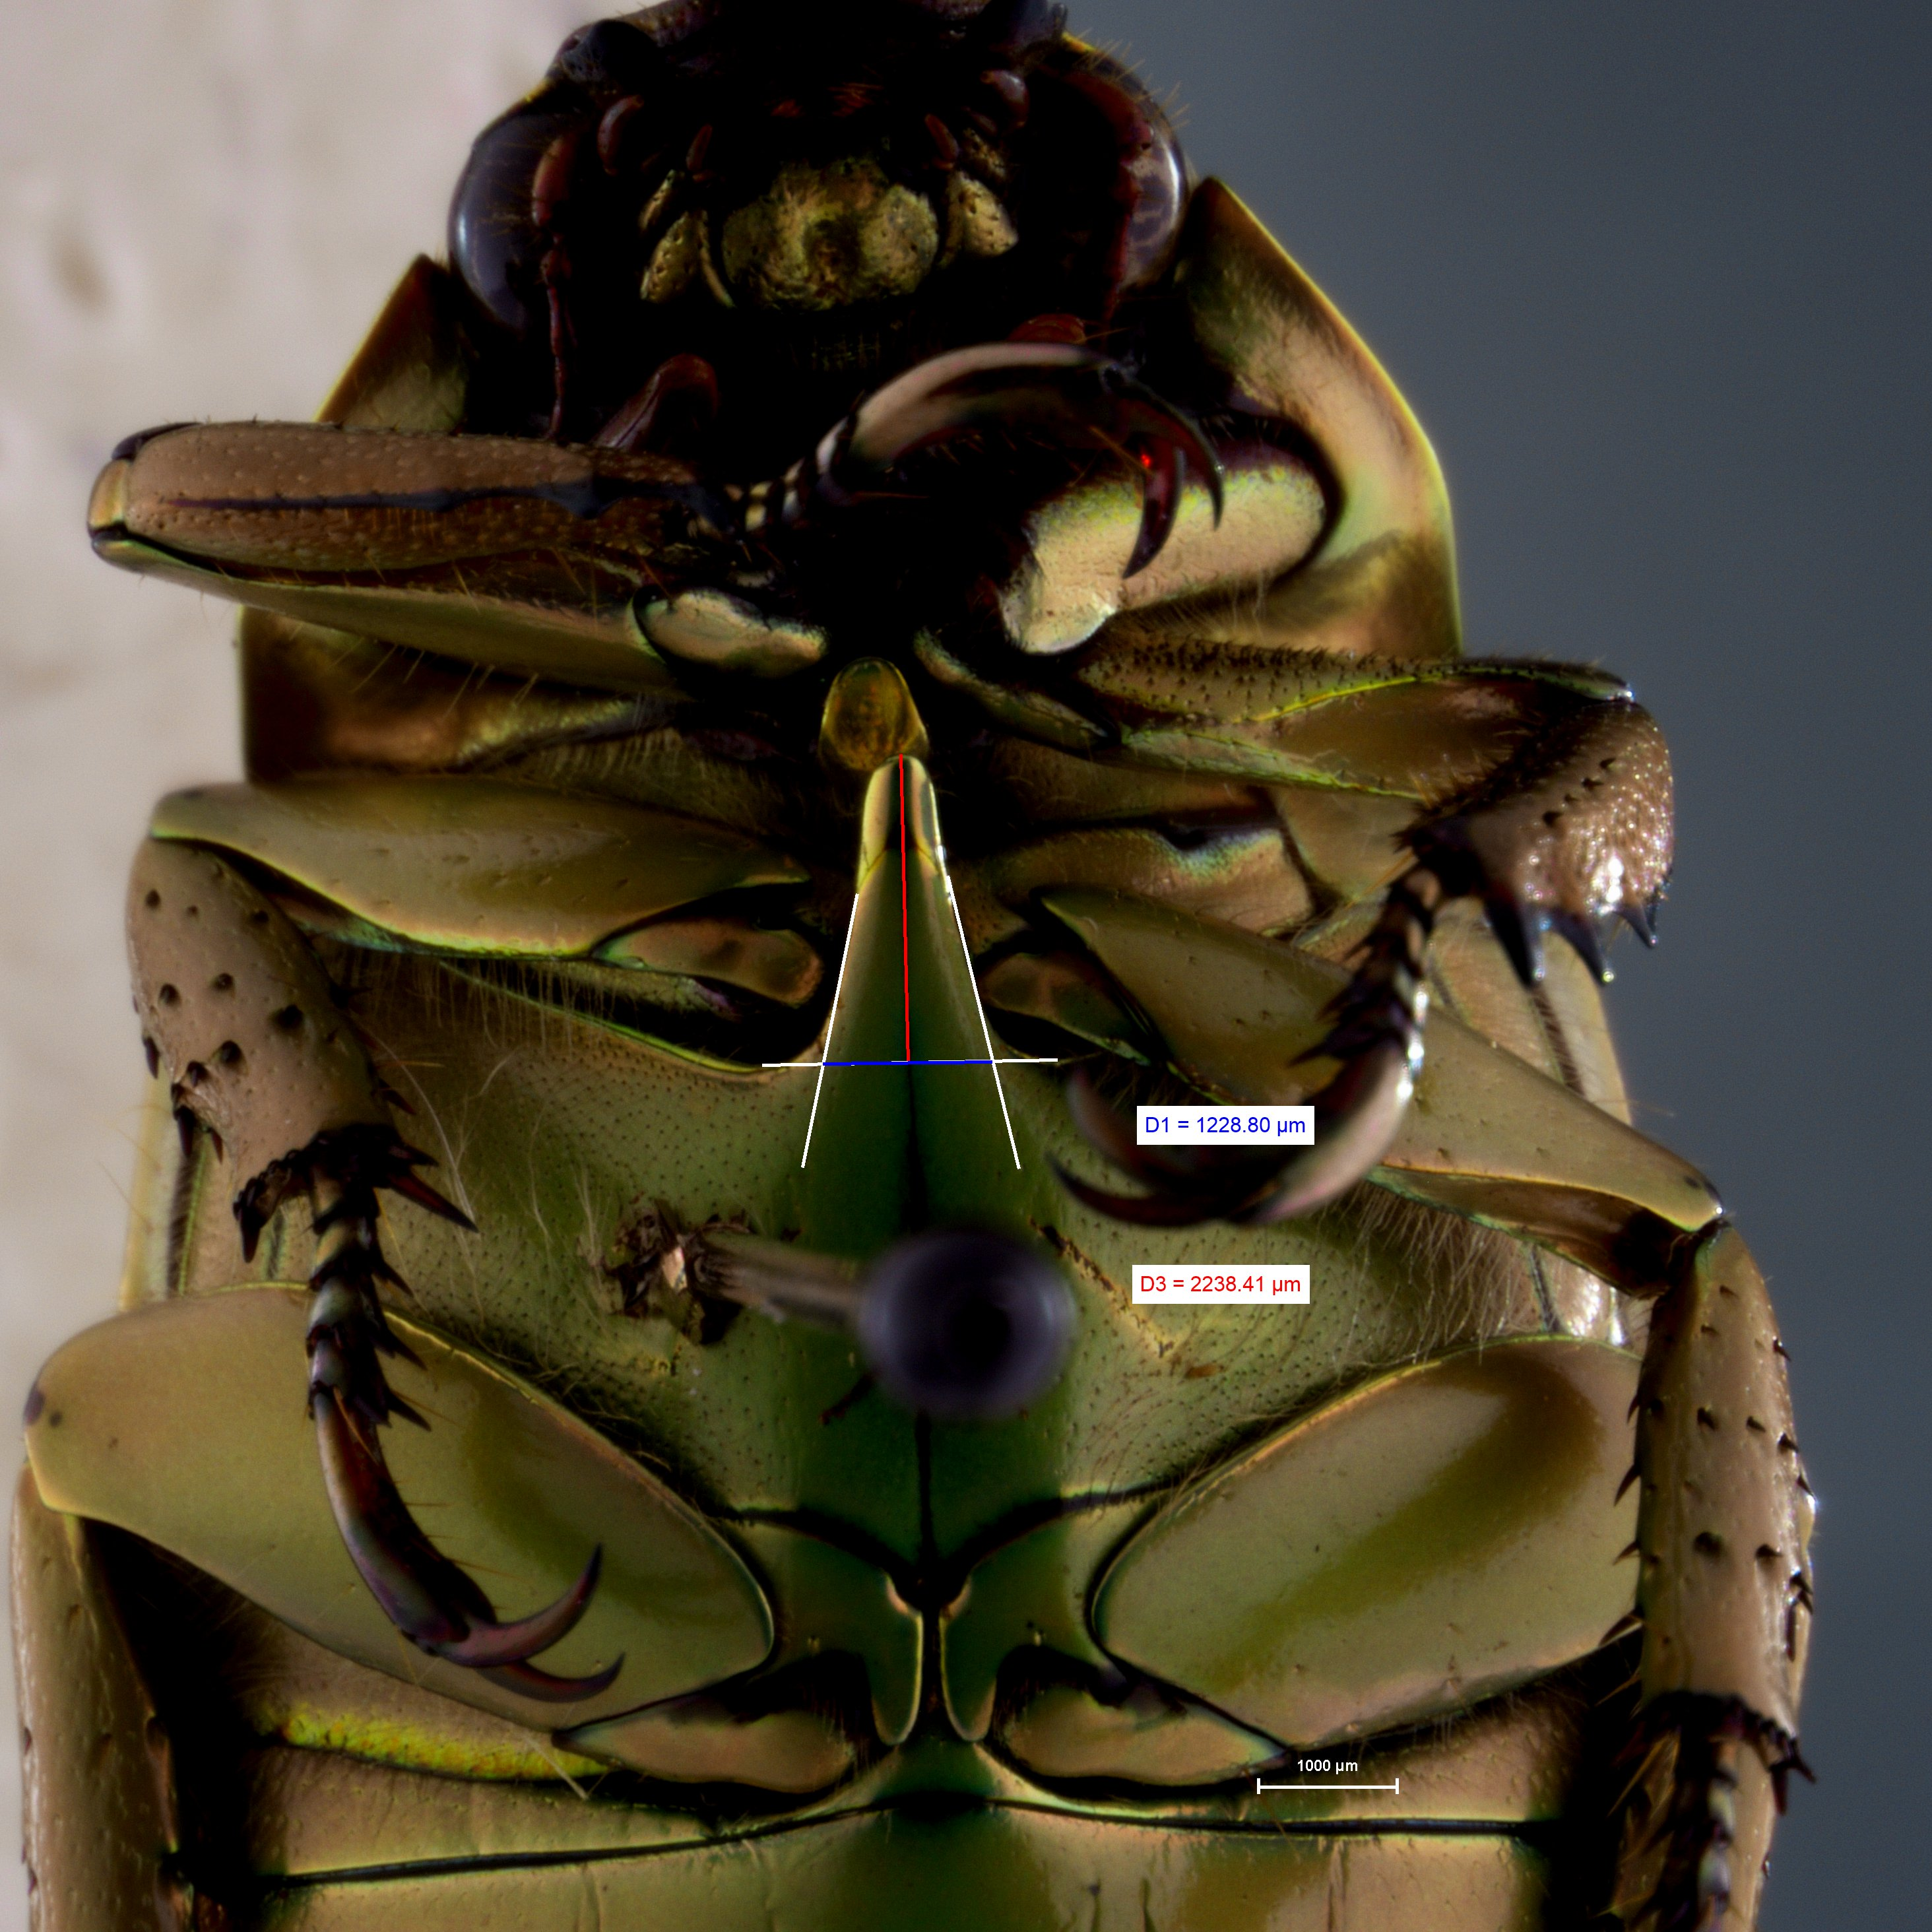
\includegraphics[width=0.5\linewidth]{images/protocol/Mesosternal_process_D3.png}
\caption{ Metric D3}
\end{figure}

\newpage
\subsection*{Metric: D4}

Vertical length from the tip of the mesosternal process down to the lowest point of the black patch in the middle of the mesosternal process

\begin{figure}[H]
\centering
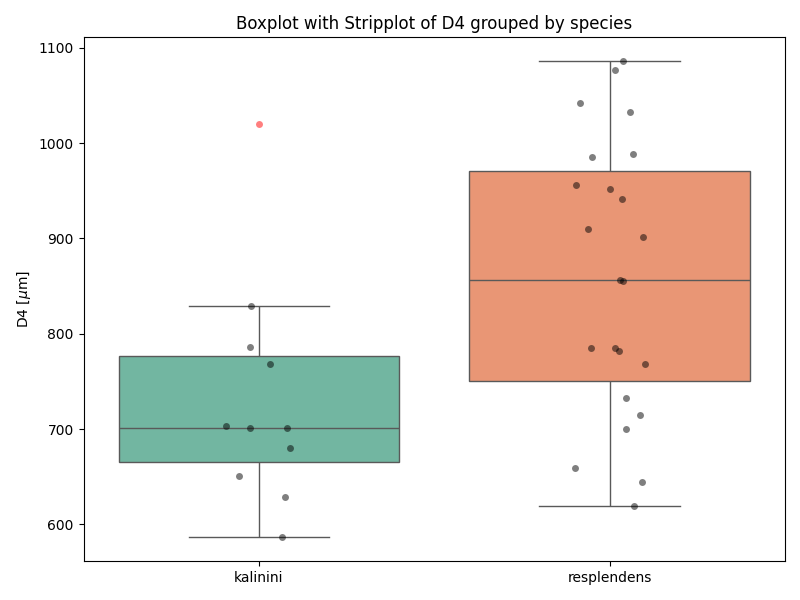
\includegraphics[width=0.7\linewidth]{images/boxplot/boxplot_D4.png}
\caption{  Boxplot and specimen distribution (superposed) for the metric  D4 by species}
\end{figure}

\noindent\textbf{Test Type:} Student's t-test \\
\noindent\textbf{Test Statistic:} -2.552 \\
\noindent\textbf{P-value:} 0.016 \\
\noindent\textbf{Interpretation:} significant difference

\begin{figure}[H]
\centering
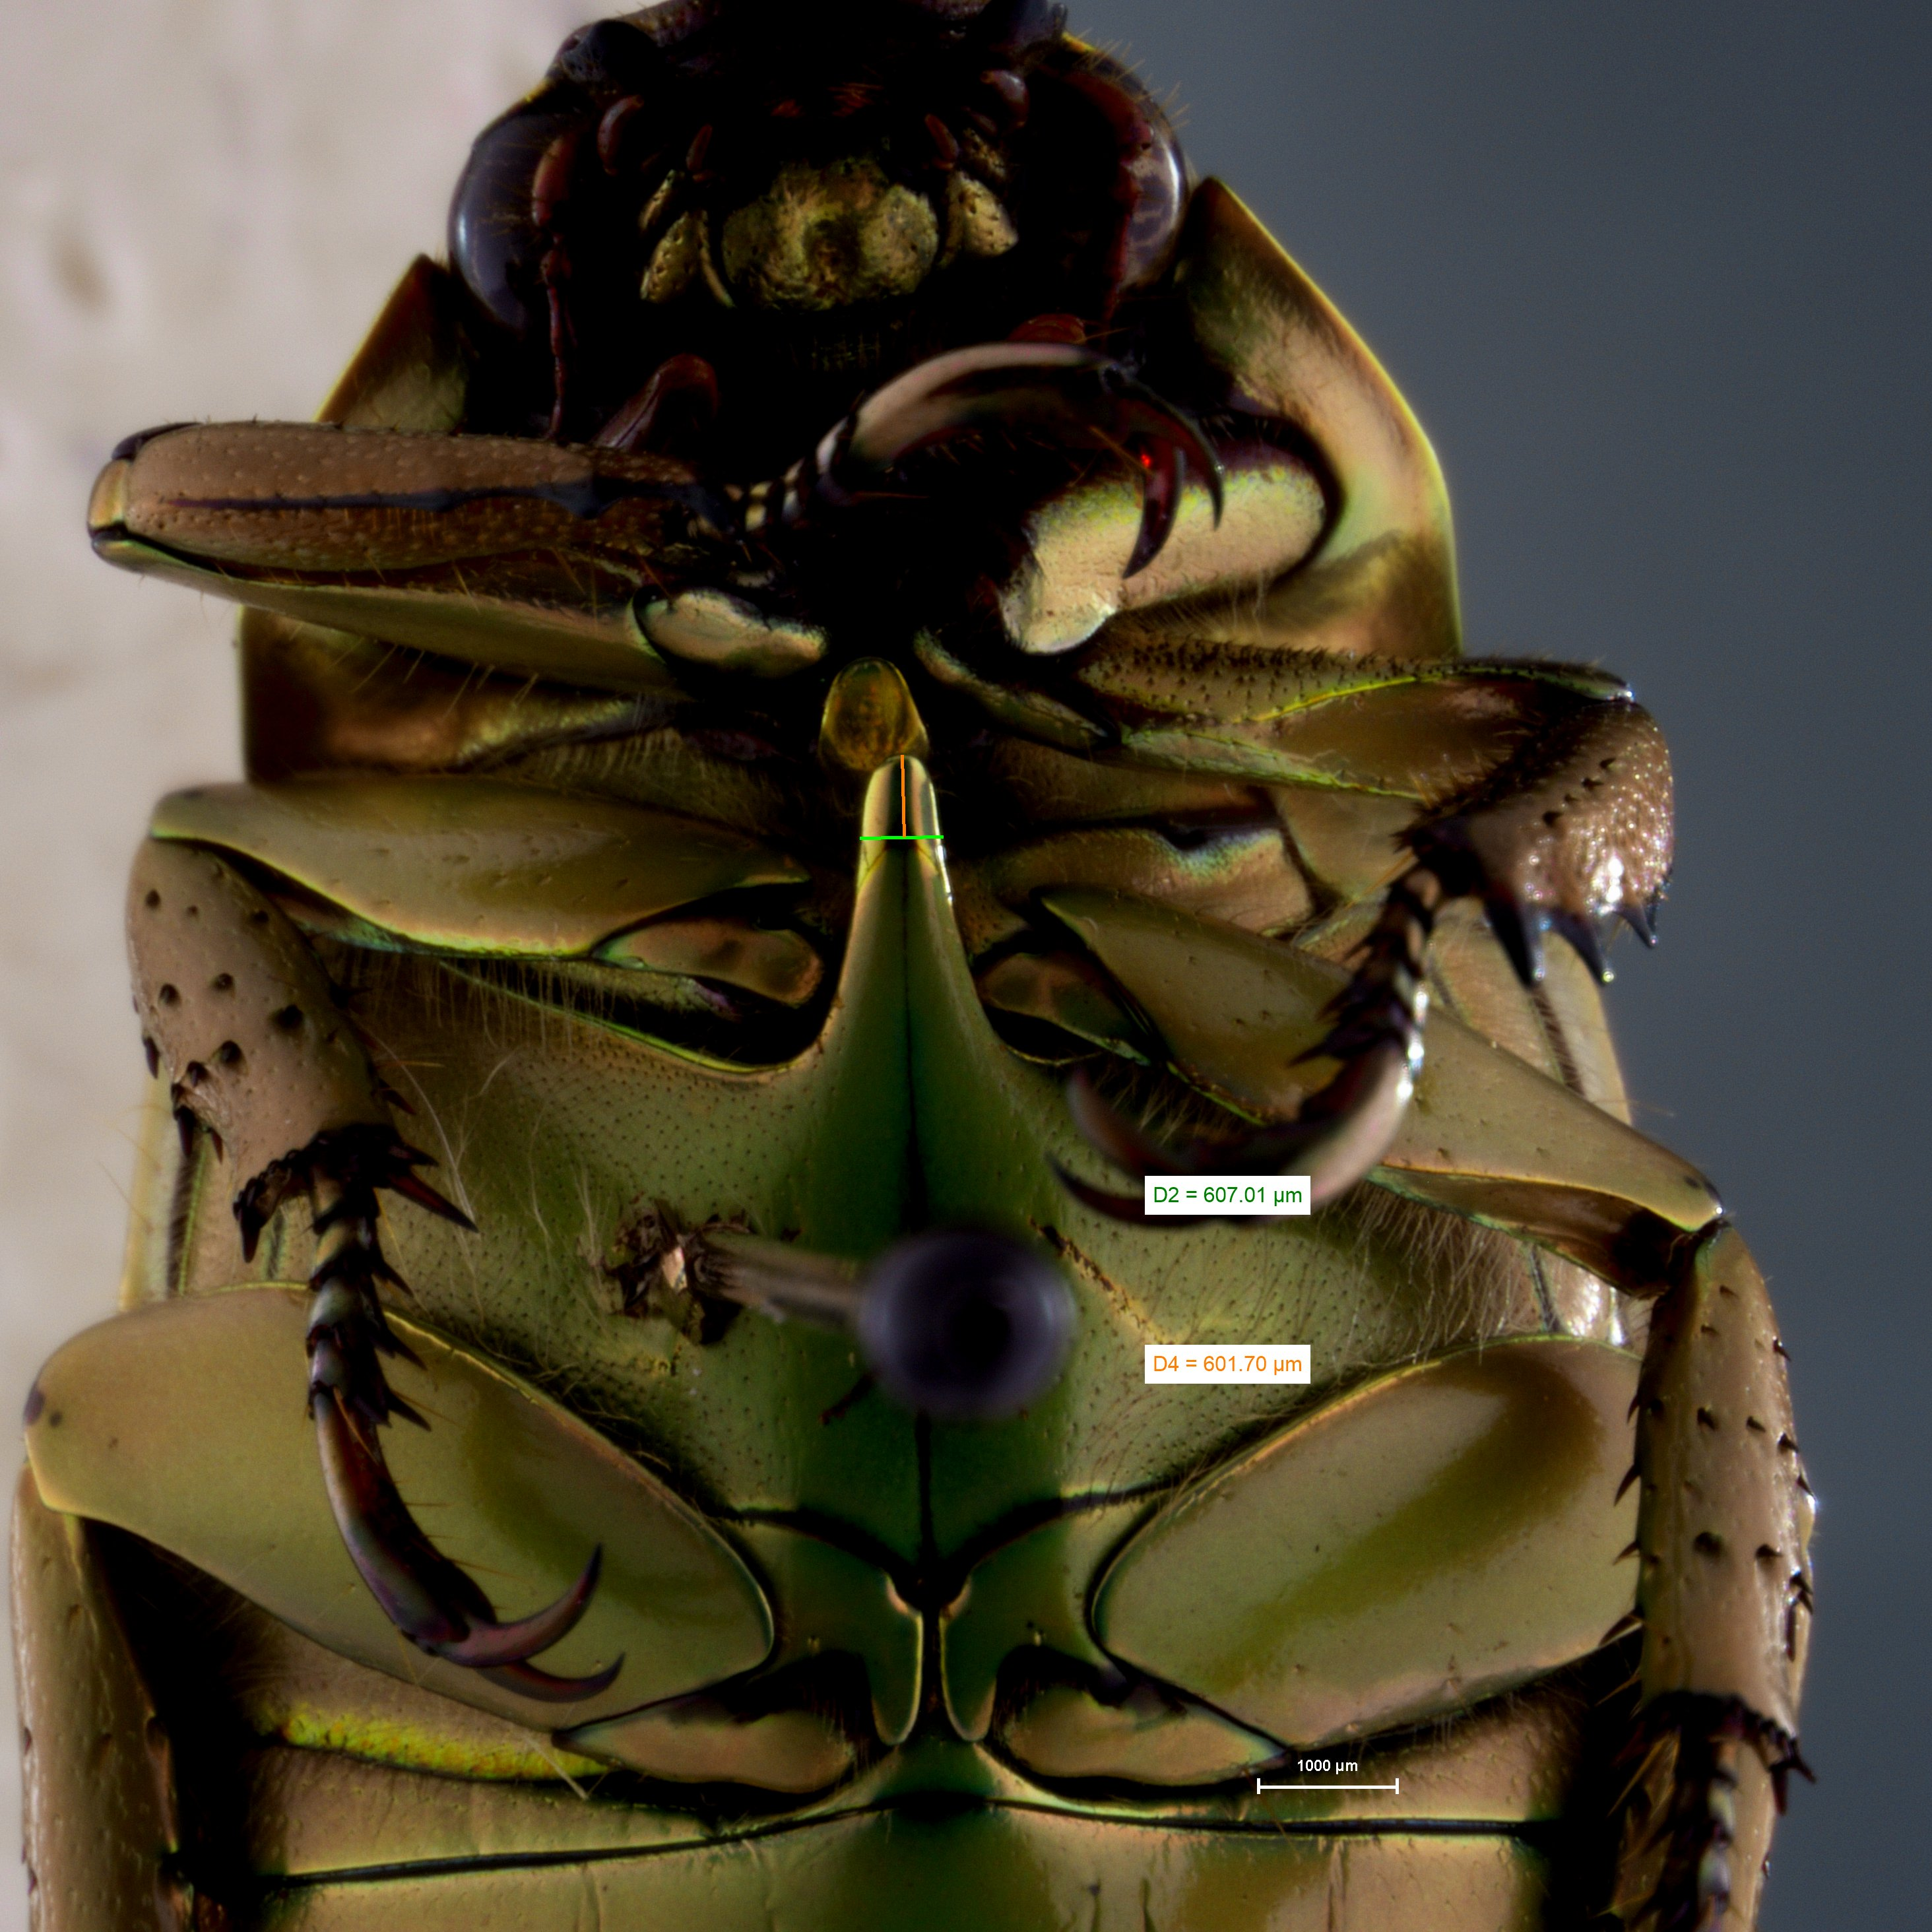
\includegraphics[width=0.5\linewidth]{images/protocol/Mesosternal_process_D4.png}
\caption{ Metric D4}
\end{figure}

\newpage
\subsection*{Metric: E1}

Horizontal top width of the prosternal plate 

\begin{figure}[H]
\centering
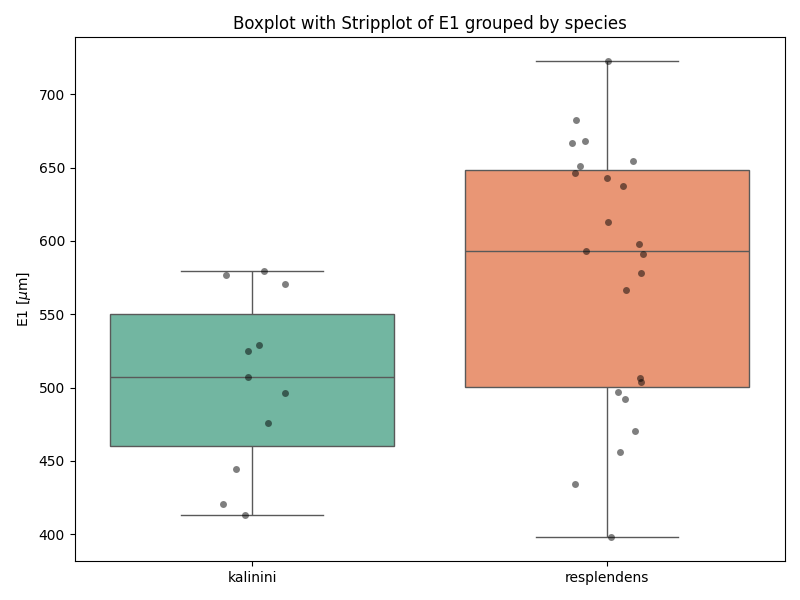
\includegraphics[width=0.7\linewidth]{images/boxplot/boxplot_E1.png}
\caption{  Boxplot and specimen distribution (superposed) for the metric  E1 by species}
\end{figure}

\noindent\textbf{Test Type:} Student's t-test \\
\noindent\textbf{Test Statistic:} -2.453 \\
\noindent\textbf{P-value:} 0.020 \\
\noindent\textbf{Interpretation:} significant difference

\begin{figure}[H]
\centering
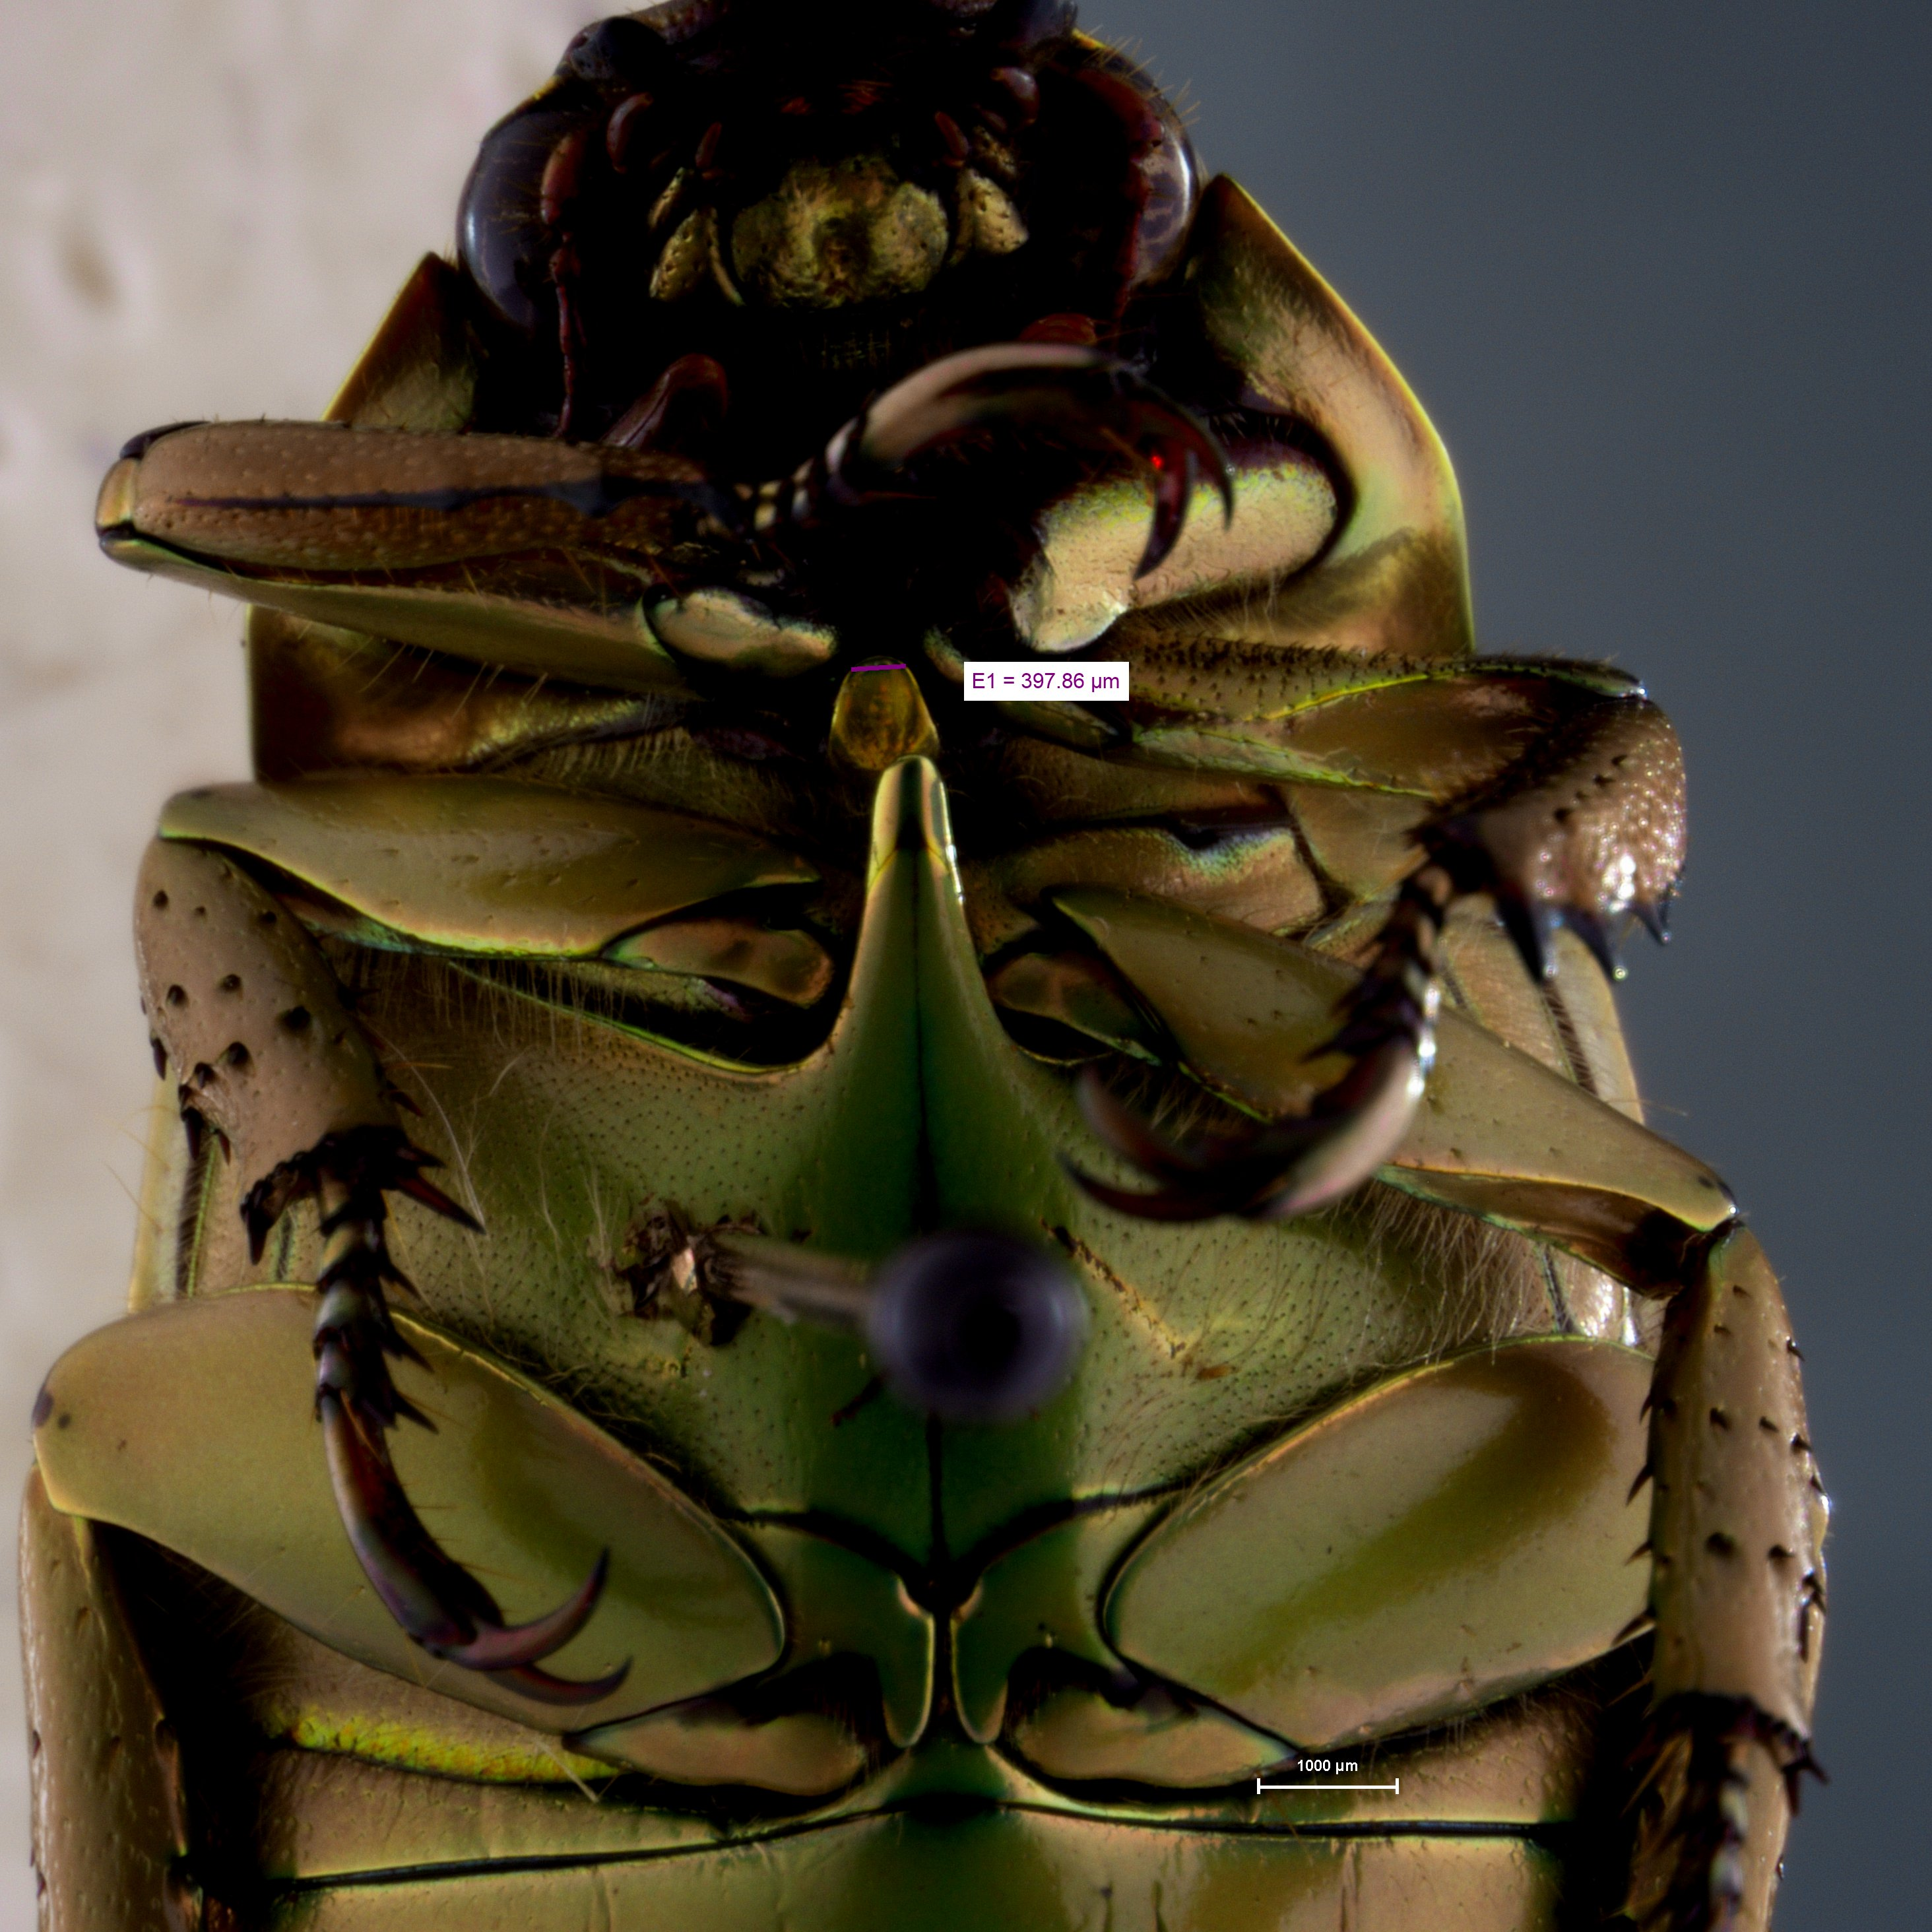
\includegraphics[width=0.5\linewidth]{images/protocol/Prosternal_process_E1.png}
\caption{ Metric E1}
\end{figure}

\newpage
\subsection*{Metric: E2}

Horizontal bottom width of the prosternal plate 

\begin{figure}[H]
\centering
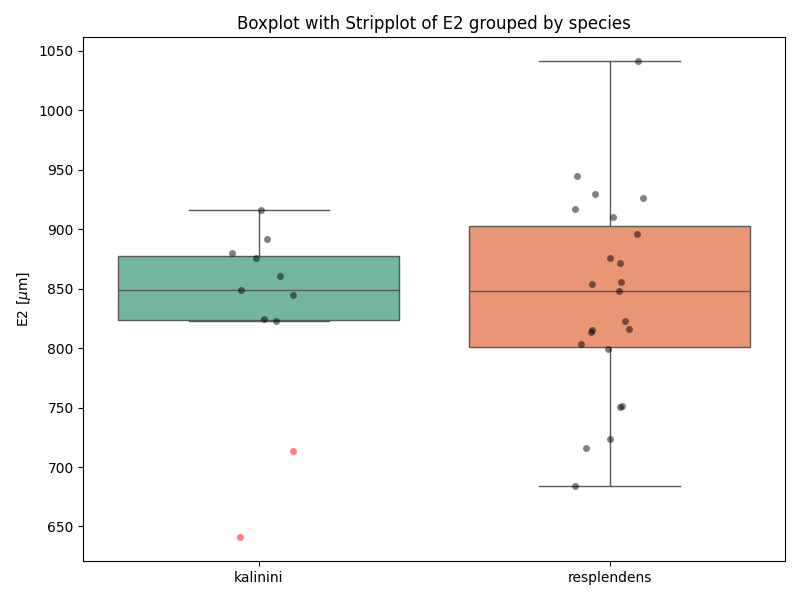
\includegraphics[width=0.7\linewidth]{images/boxplot/boxplot_E2.png}
\caption{  Boxplot and specimen distribution (superposed) for the metric  E2 by species}
\end{figure}

\noindent\textbf{Test Type:} Mann-Whitney U test \\
\noindent\textbf{Test Statistic:} 124.000 \\
\noindent\textbf{P-value:} 0.941 \\
\noindent\textbf{Interpretation:} no significant difference

\begin{figure}[H]
\centering
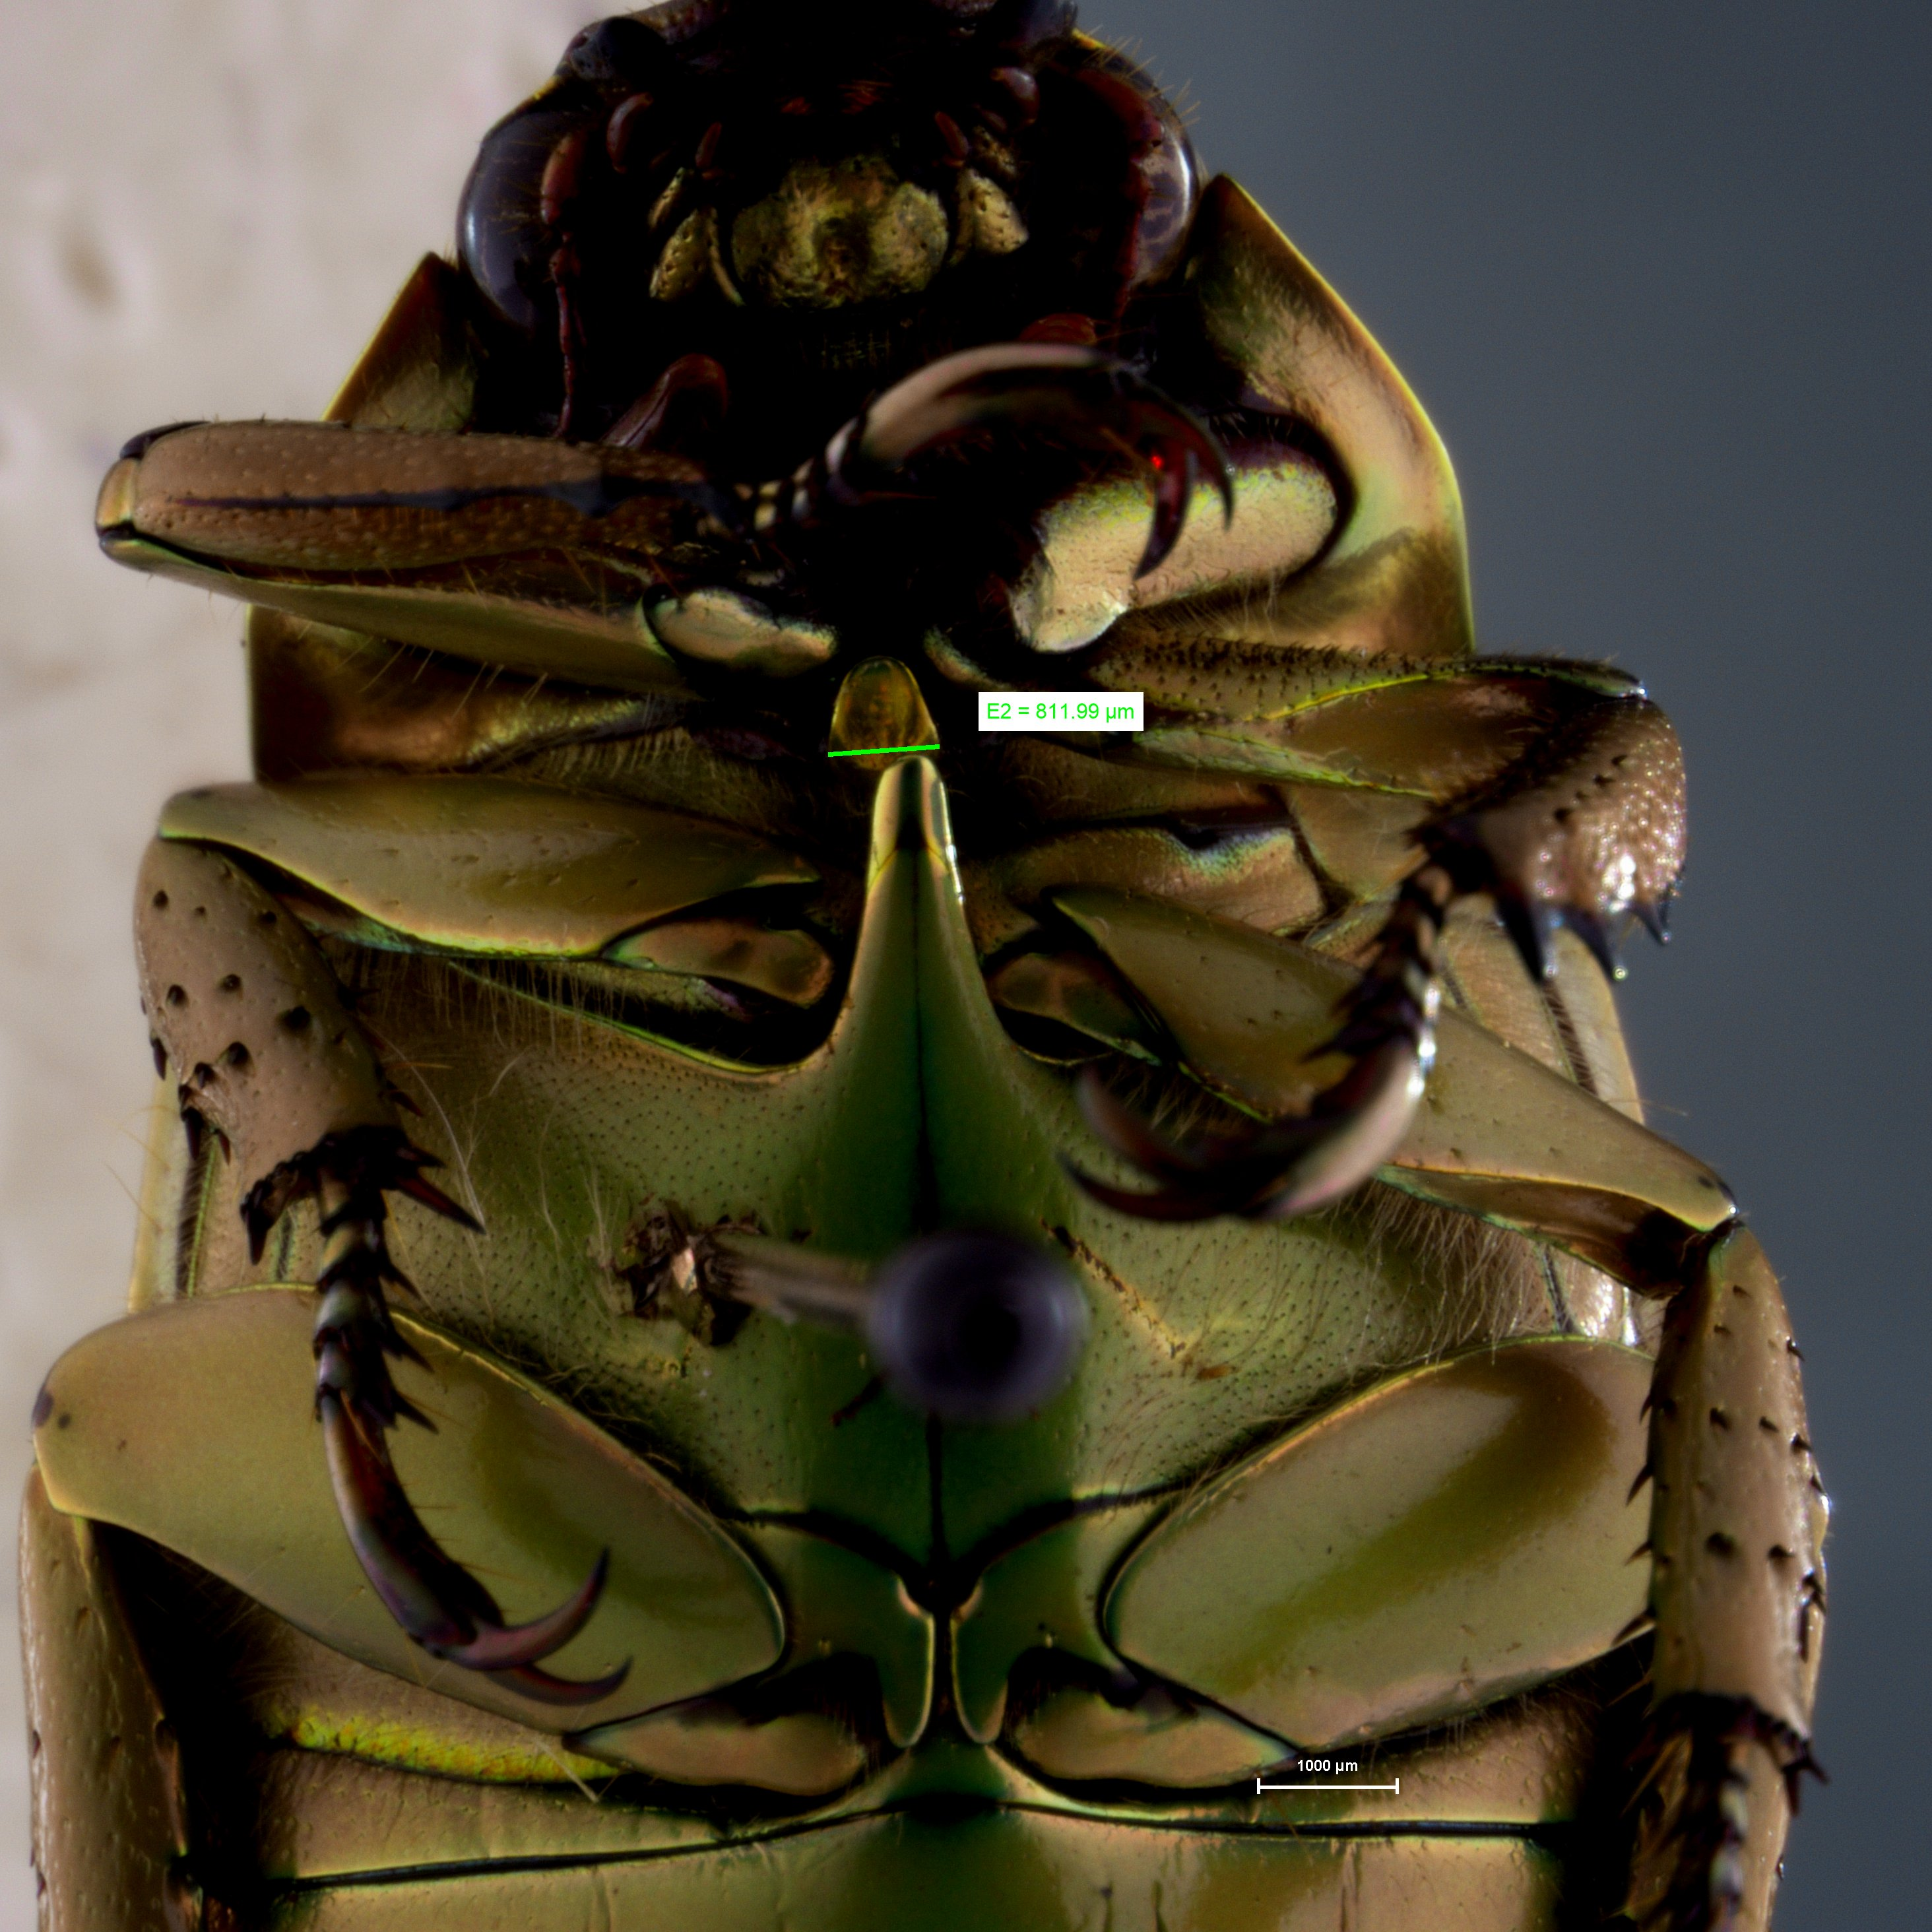
\includegraphics[width=0.5\linewidth]{images/protocol/Prosternal_process_E2.png}
\caption{ Metric E2}
\end{figure}

\newpage
\subsection*{Metric: F1}

Vertical length of the foremost ventral plate

\begin{figure}[H]
\centering
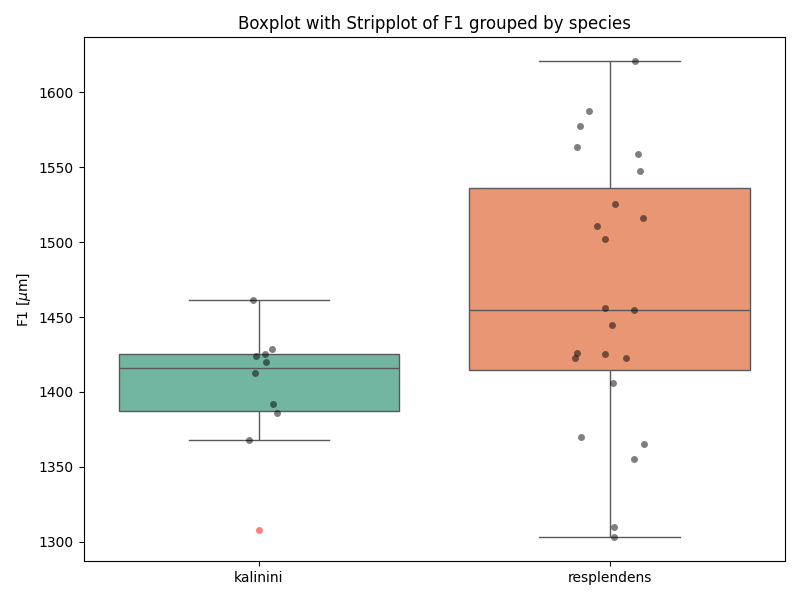
\includegraphics[width=0.7\linewidth]{images/boxplot/boxplot_F1.png}
\caption{  Boxplot and specimen distribution (superposed) for the metric  F1 by species}
\end{figure}

\noindent\textbf{Test Type:} Welch's t-test \\
\noindent\textbf{Test Statistic:} -2.665 \\
\noindent\textbf{P-value:} 0.012 \\
\noindent\textbf{Interpretation:} significant difference

\begin{figure}[H]
\centering
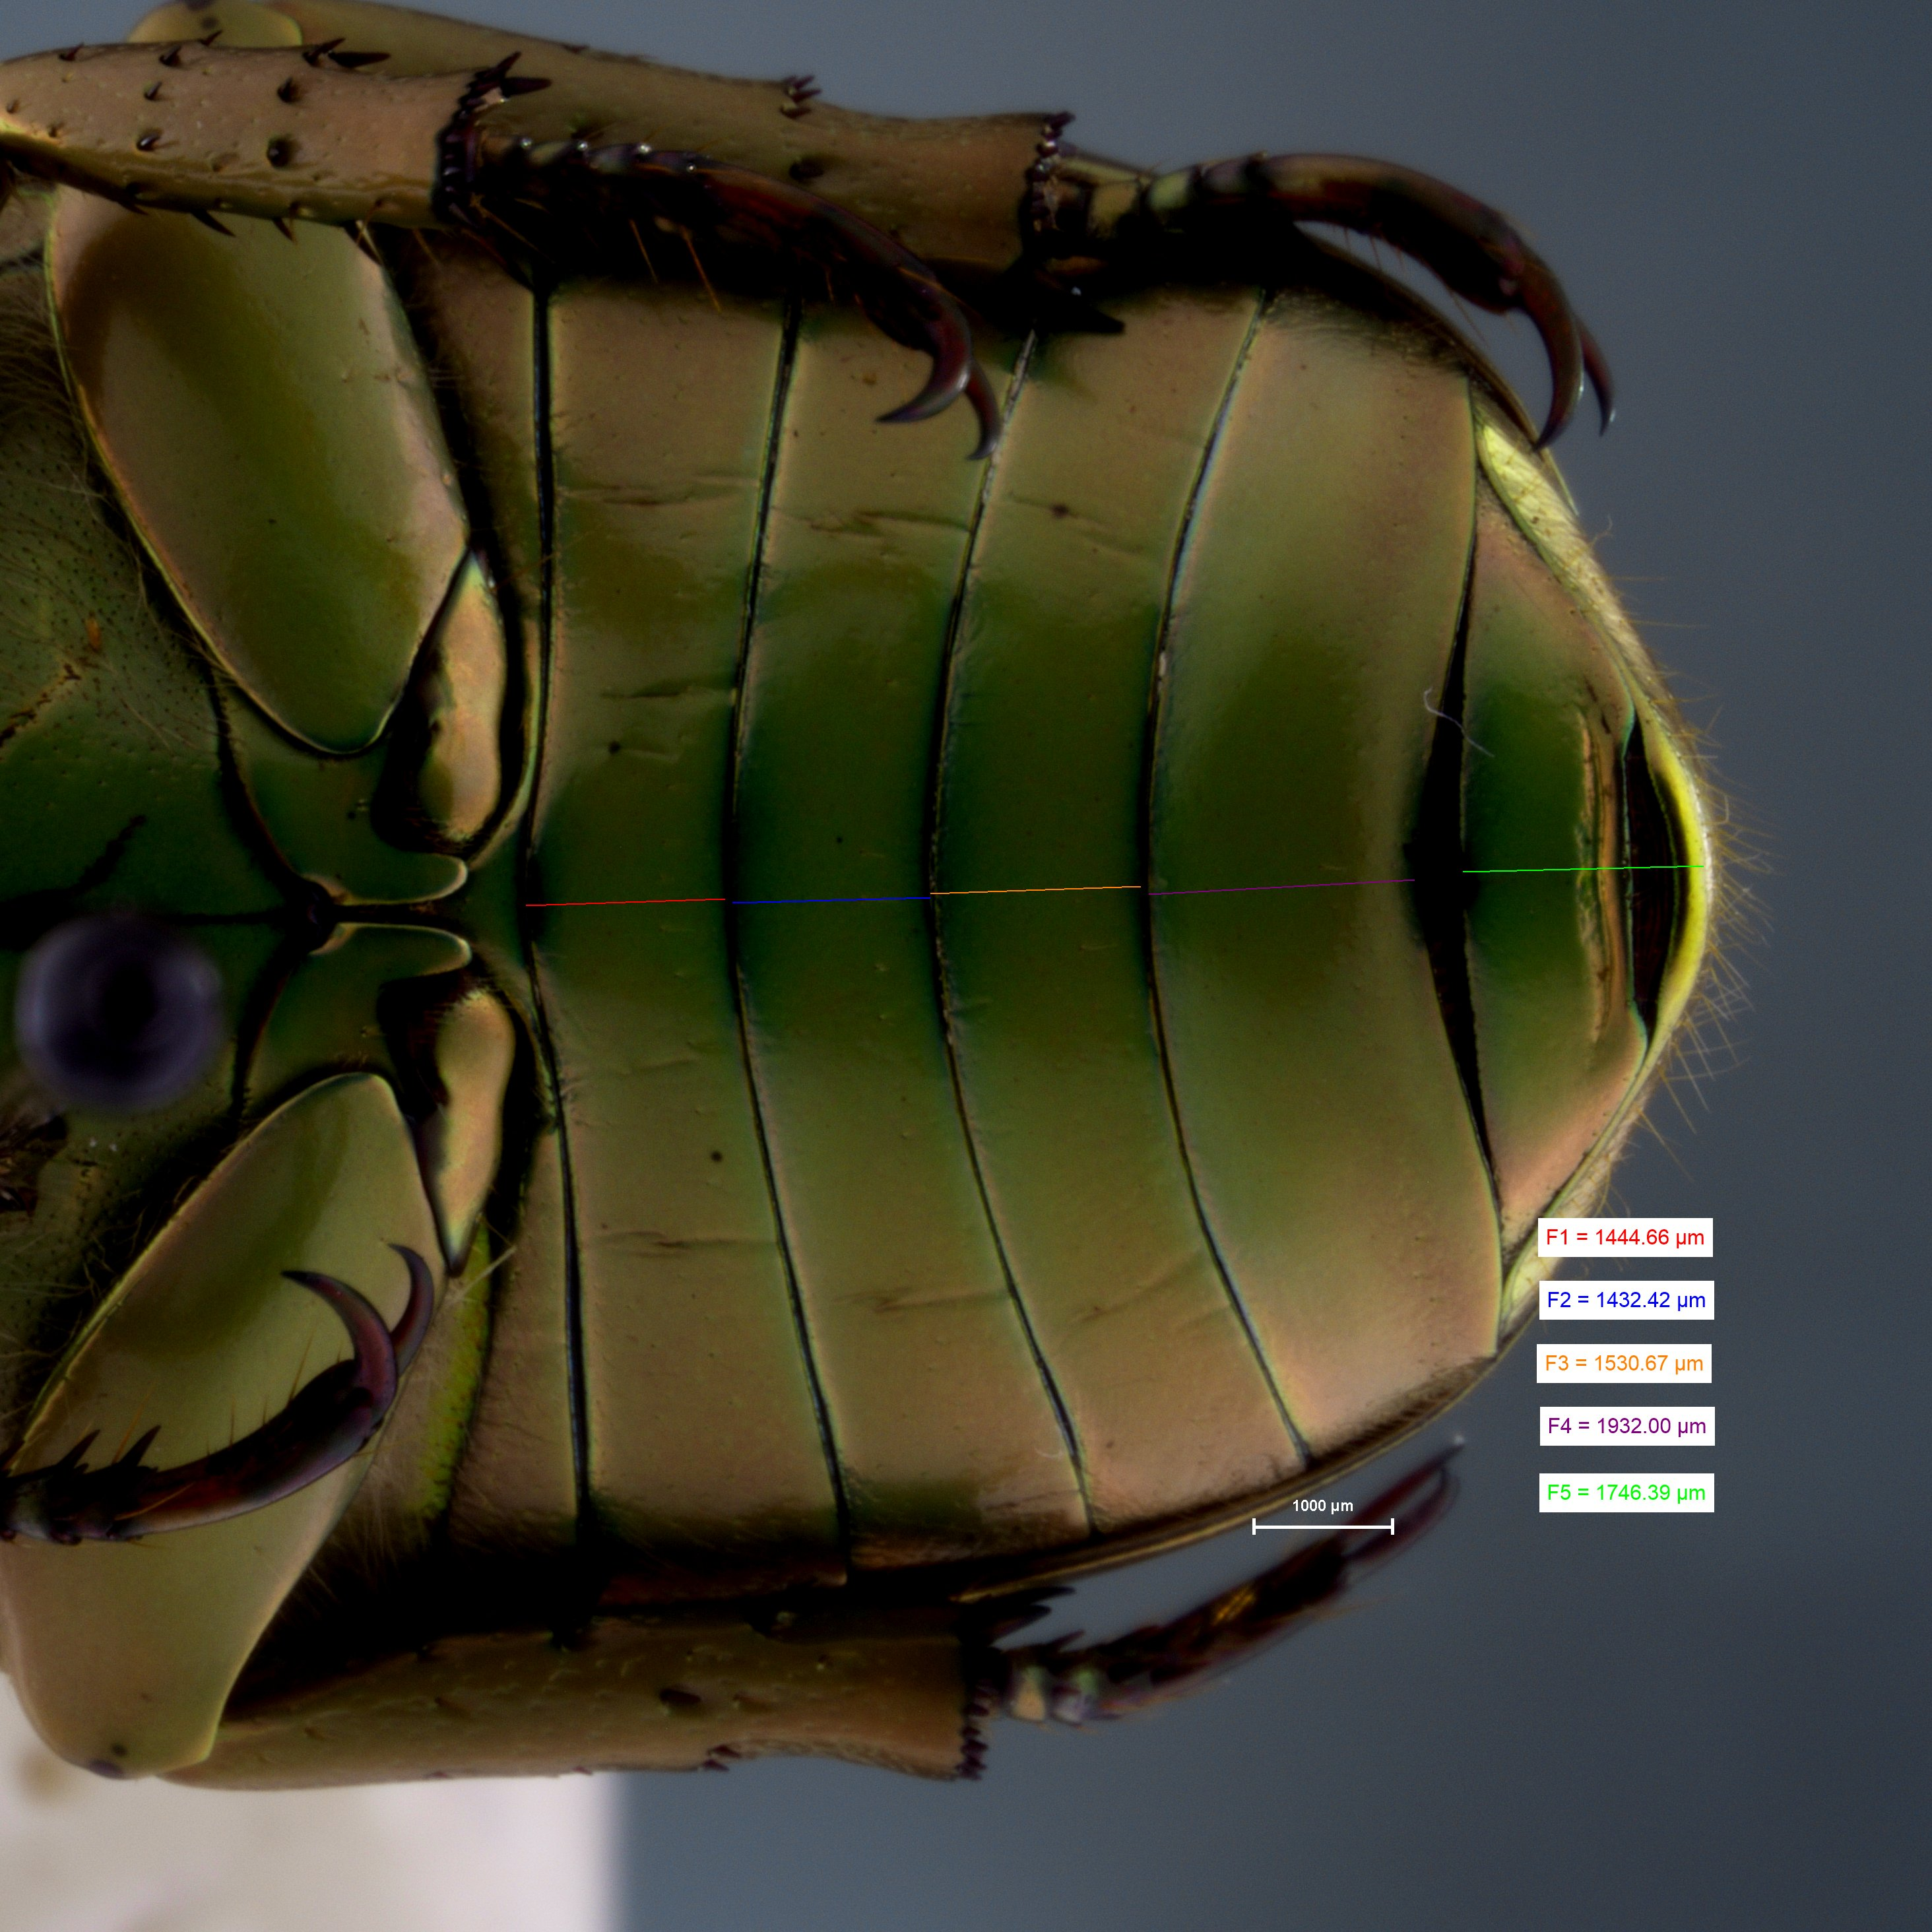
\includegraphics[width=0.5\linewidth]{images/protocol/Ventral.png}
\caption{ Metric F1}
\end{figure}

\newpage
\subsection*{Metric: F2}

Vertical length of the second foremost ventral plate

\begin{figure}[H]
\centering
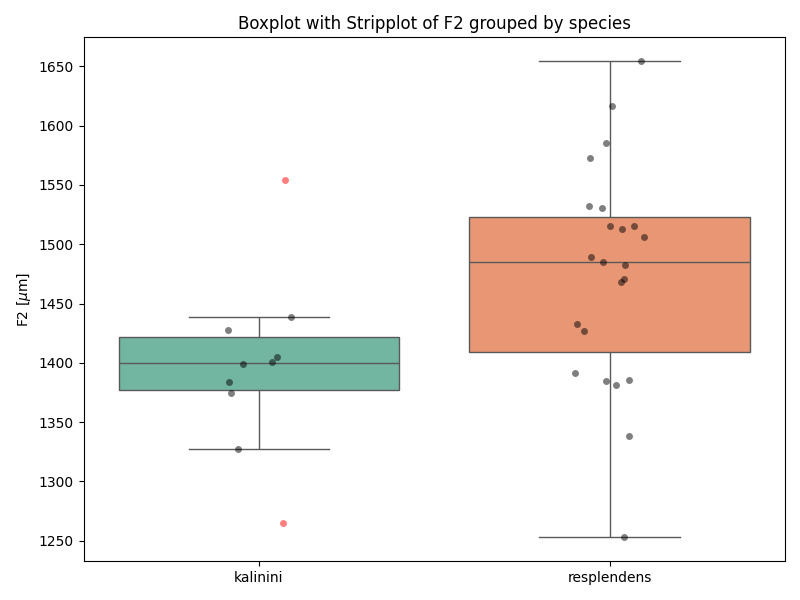
\includegraphics[width=0.7\linewidth]{images/boxplot/boxplot_F2.png}
\caption{  Boxplot and specimen distribution (superposed) for the metric  F2 by species}
\end{figure}

\noindent\textbf{Test Type:} Student's t-test \\
\noindent\textbf{Test Statistic:} -2.331 \\
\noindent\textbf{P-value:} 0.026 \\
\noindent\textbf{Interpretation:} significant difference

\begin{figure}[H]
\centering
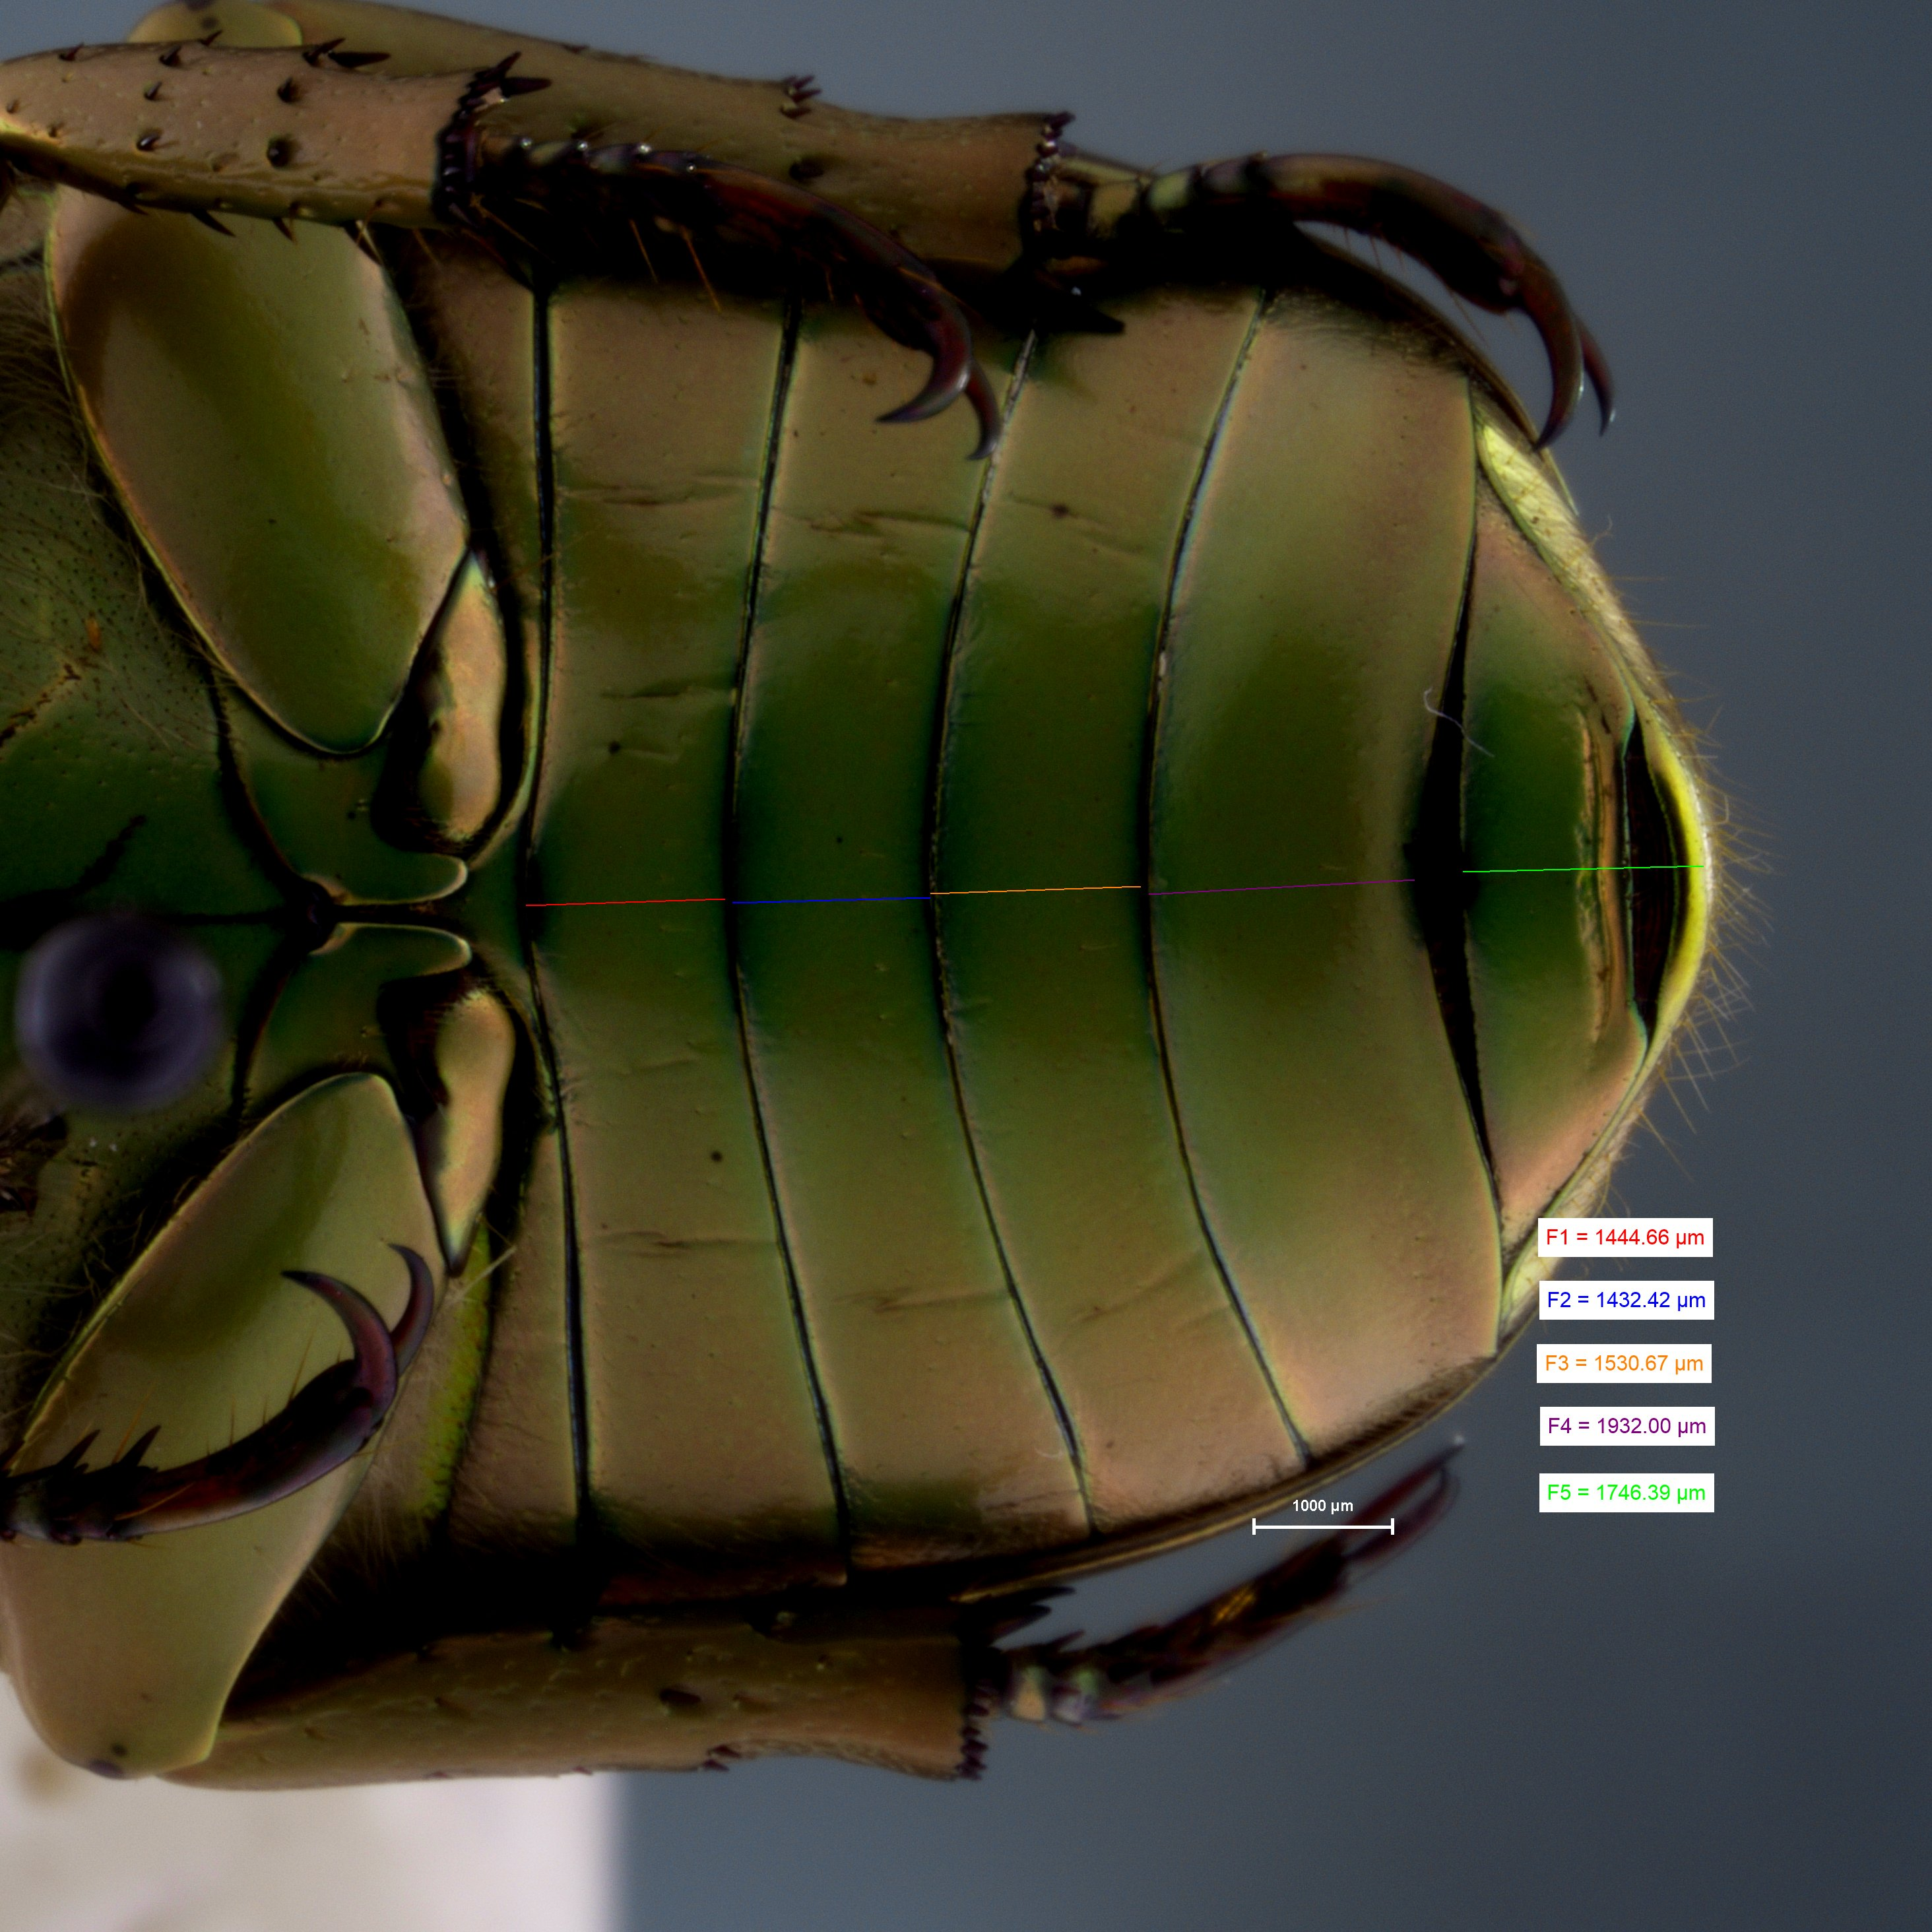
\includegraphics[width=0.5\linewidth]{images/protocol/Ventral.png}
\caption{ Metric F2}
\end{figure}

\newpage
\subsection*{Metric: F3}

Vertical length of the third foremost ventral plate

\begin{figure}[H]
\centering
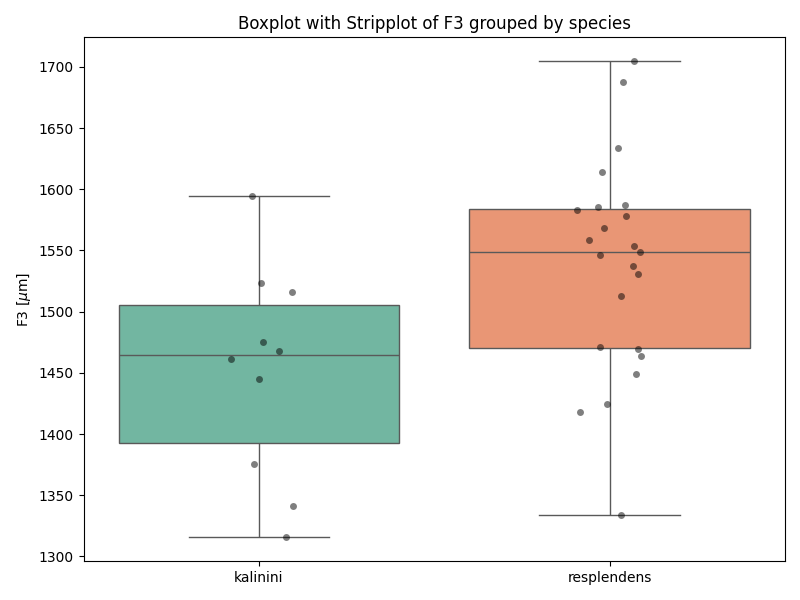
\includegraphics[width=0.7\linewidth]{images/boxplot/boxplot_F3.png}
\caption{  Boxplot and specimen distribution (superposed) for the metric  F3 by species}
\end{figure}

\noindent\textbf{Test Type:} Student's t-test \\
\noindent\textbf{Test Statistic:} -2.605 \\
\noindent\textbf{P-value:} 0.014 \\
\noindent\textbf{Interpretation:} significant difference

\begin{figure}[H]
\centering
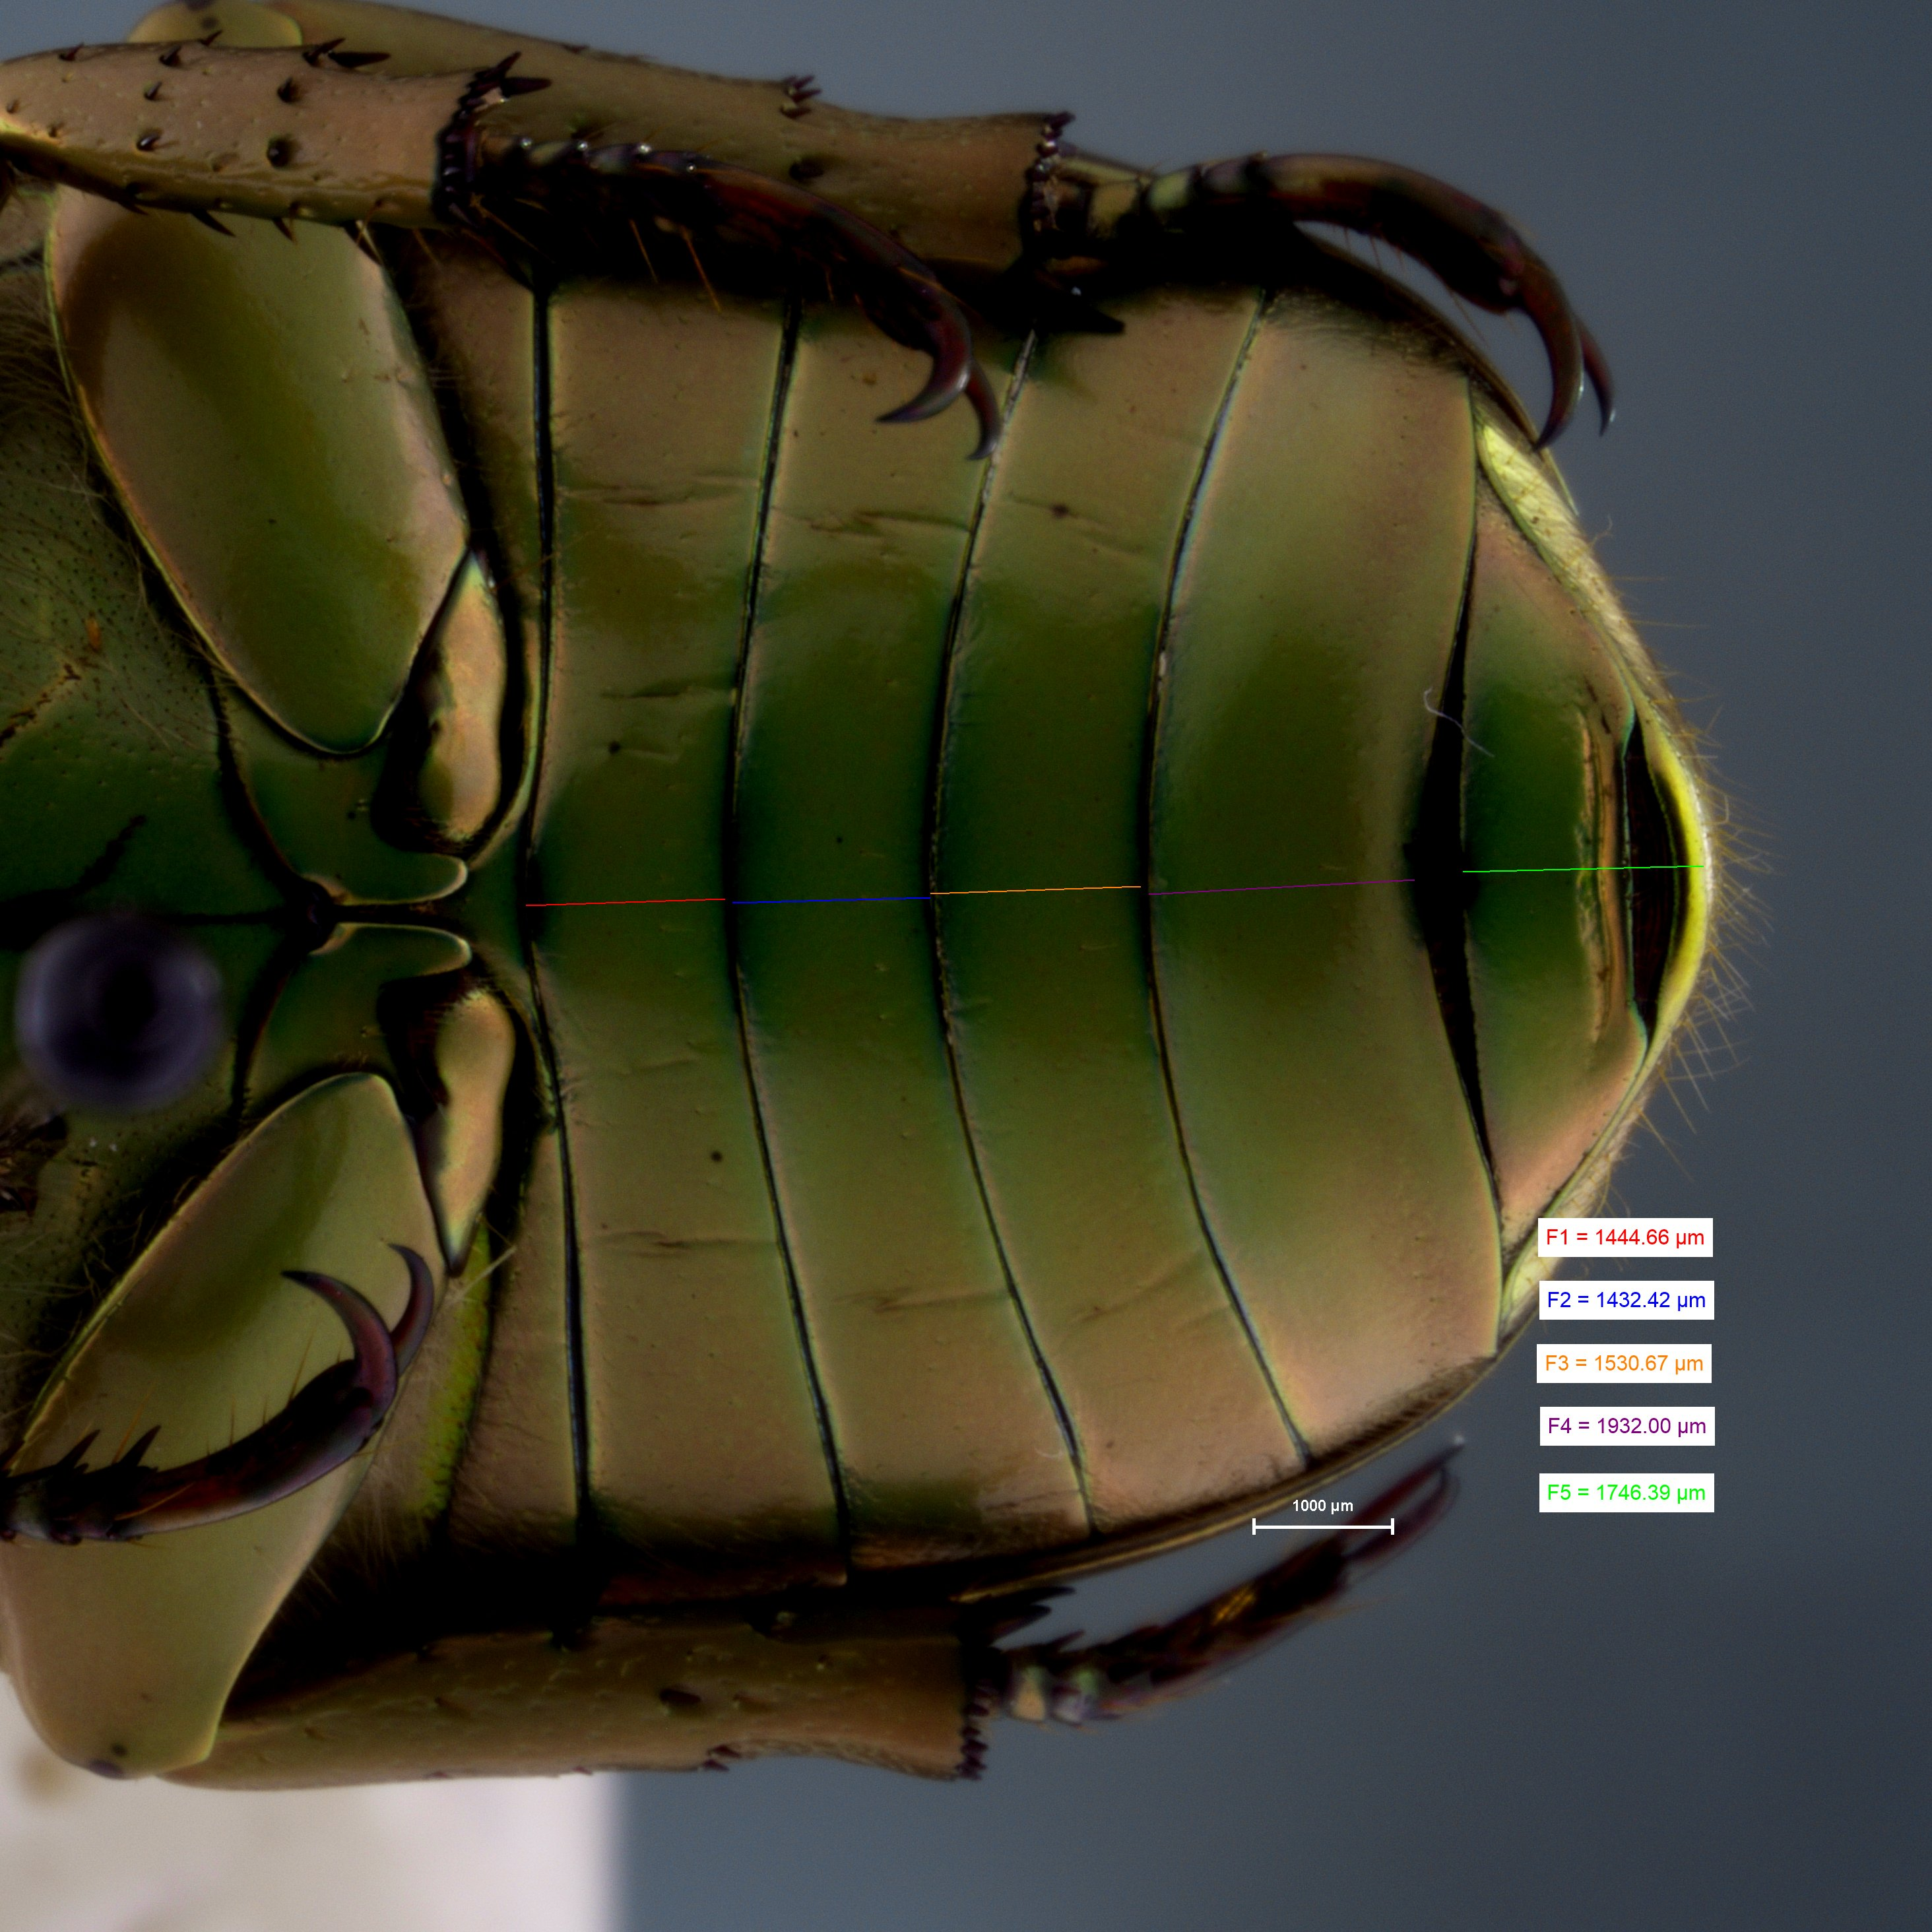
\includegraphics[width=0.5\linewidth]{images/protocol/Ventral.png}
\caption{ Metric F3}
\end{figure}

\newpage
\subsection*{Metric: F4}

Vertical length of the fourth foremost ventral plate 

\begin{figure}[H]
\centering
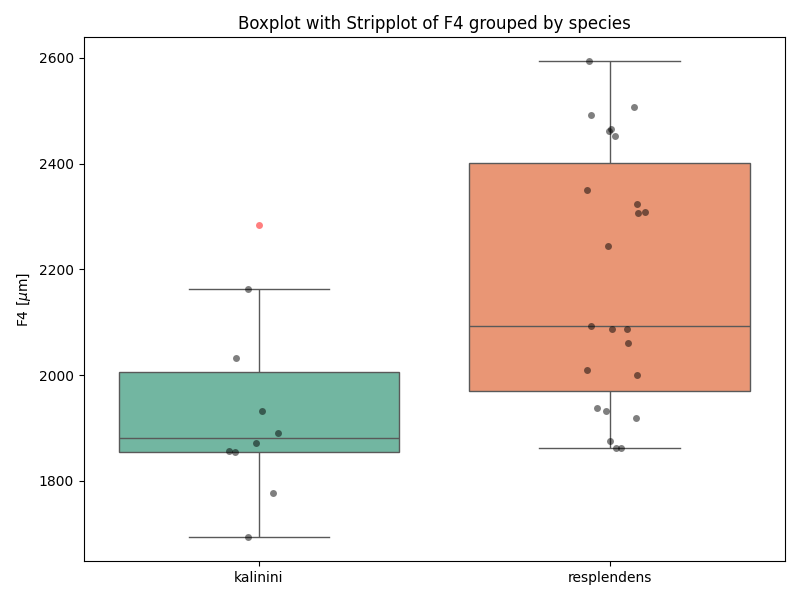
\includegraphics[width=0.7\linewidth]{images/boxplot/boxplot_F4.png}
\caption{  Boxplot and specimen distribution (superposed) for the metric  F4 by species}
\end{figure}

\noindent\textbf{Test Type:} Student's t-test \\
\noindent\textbf{Test Statistic:} -2.925 \\
\noindent\textbf{P-value:} 0.006 \\
\noindent\textbf{Interpretation:} significant difference

\begin{figure}[H]
\centering
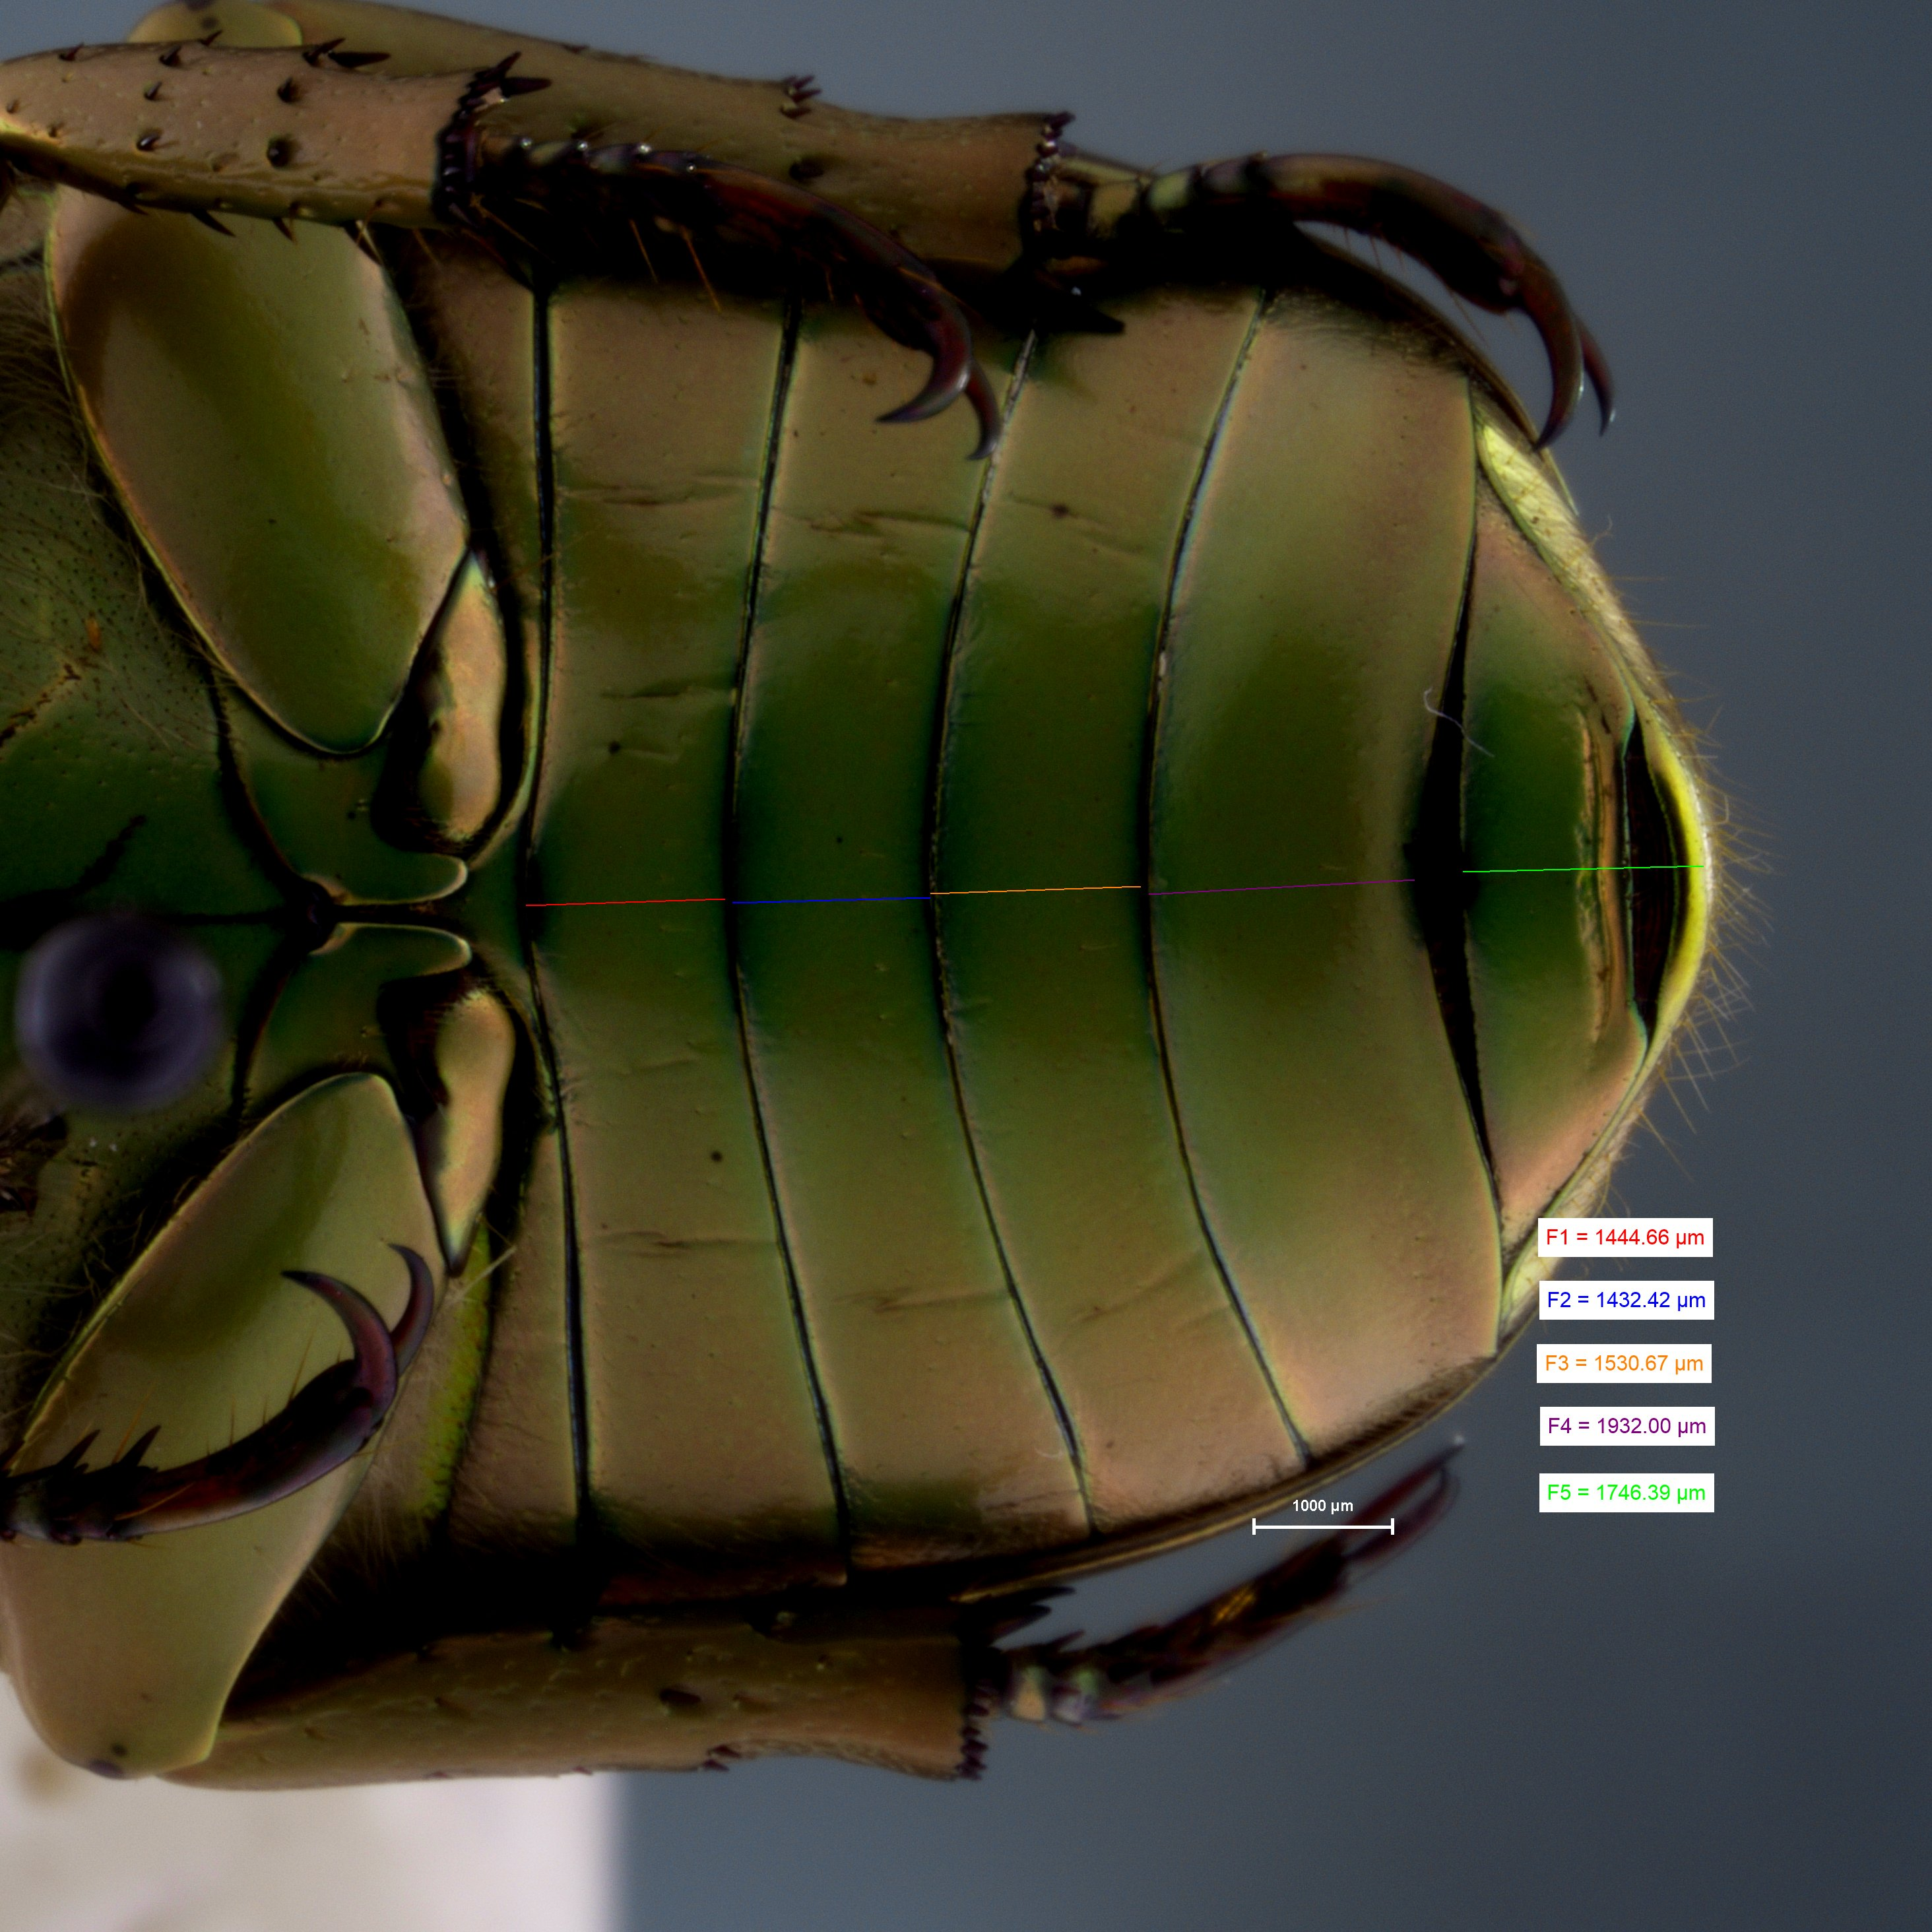
\includegraphics[width=0.5\linewidth]{images/protocol/Ventral.png}
\caption{ Metric F4}
\end{figure}

\newpage
\subsection*{Metric: F5}

Vertical length of the fifth foremost ventral plate

\begin{figure}[H]
\centering
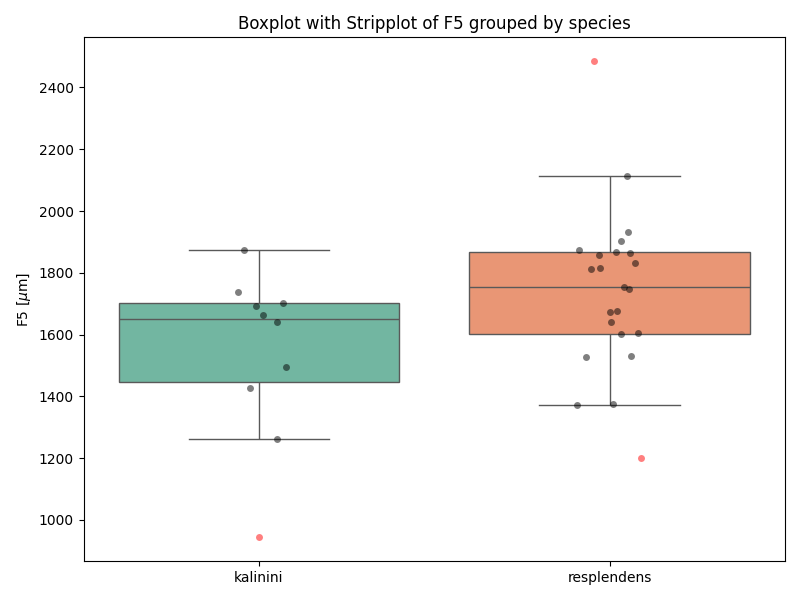
\includegraphics[width=0.7\linewidth]{images/boxplot/boxplot_F5.png}
\caption{  Boxplot and specimen distribution (superposed) for the metric  F5 by species}
\end{figure}

\noindent\textbf{Test Type:} Student's t-test \\
\noindent\textbf{Test Statistic:} -1.949 \\
\noindent\textbf{P-value:} 0.060 \\
\noindent\textbf{Interpretation:} no significant difference

\begin{figure}[H]
\centering
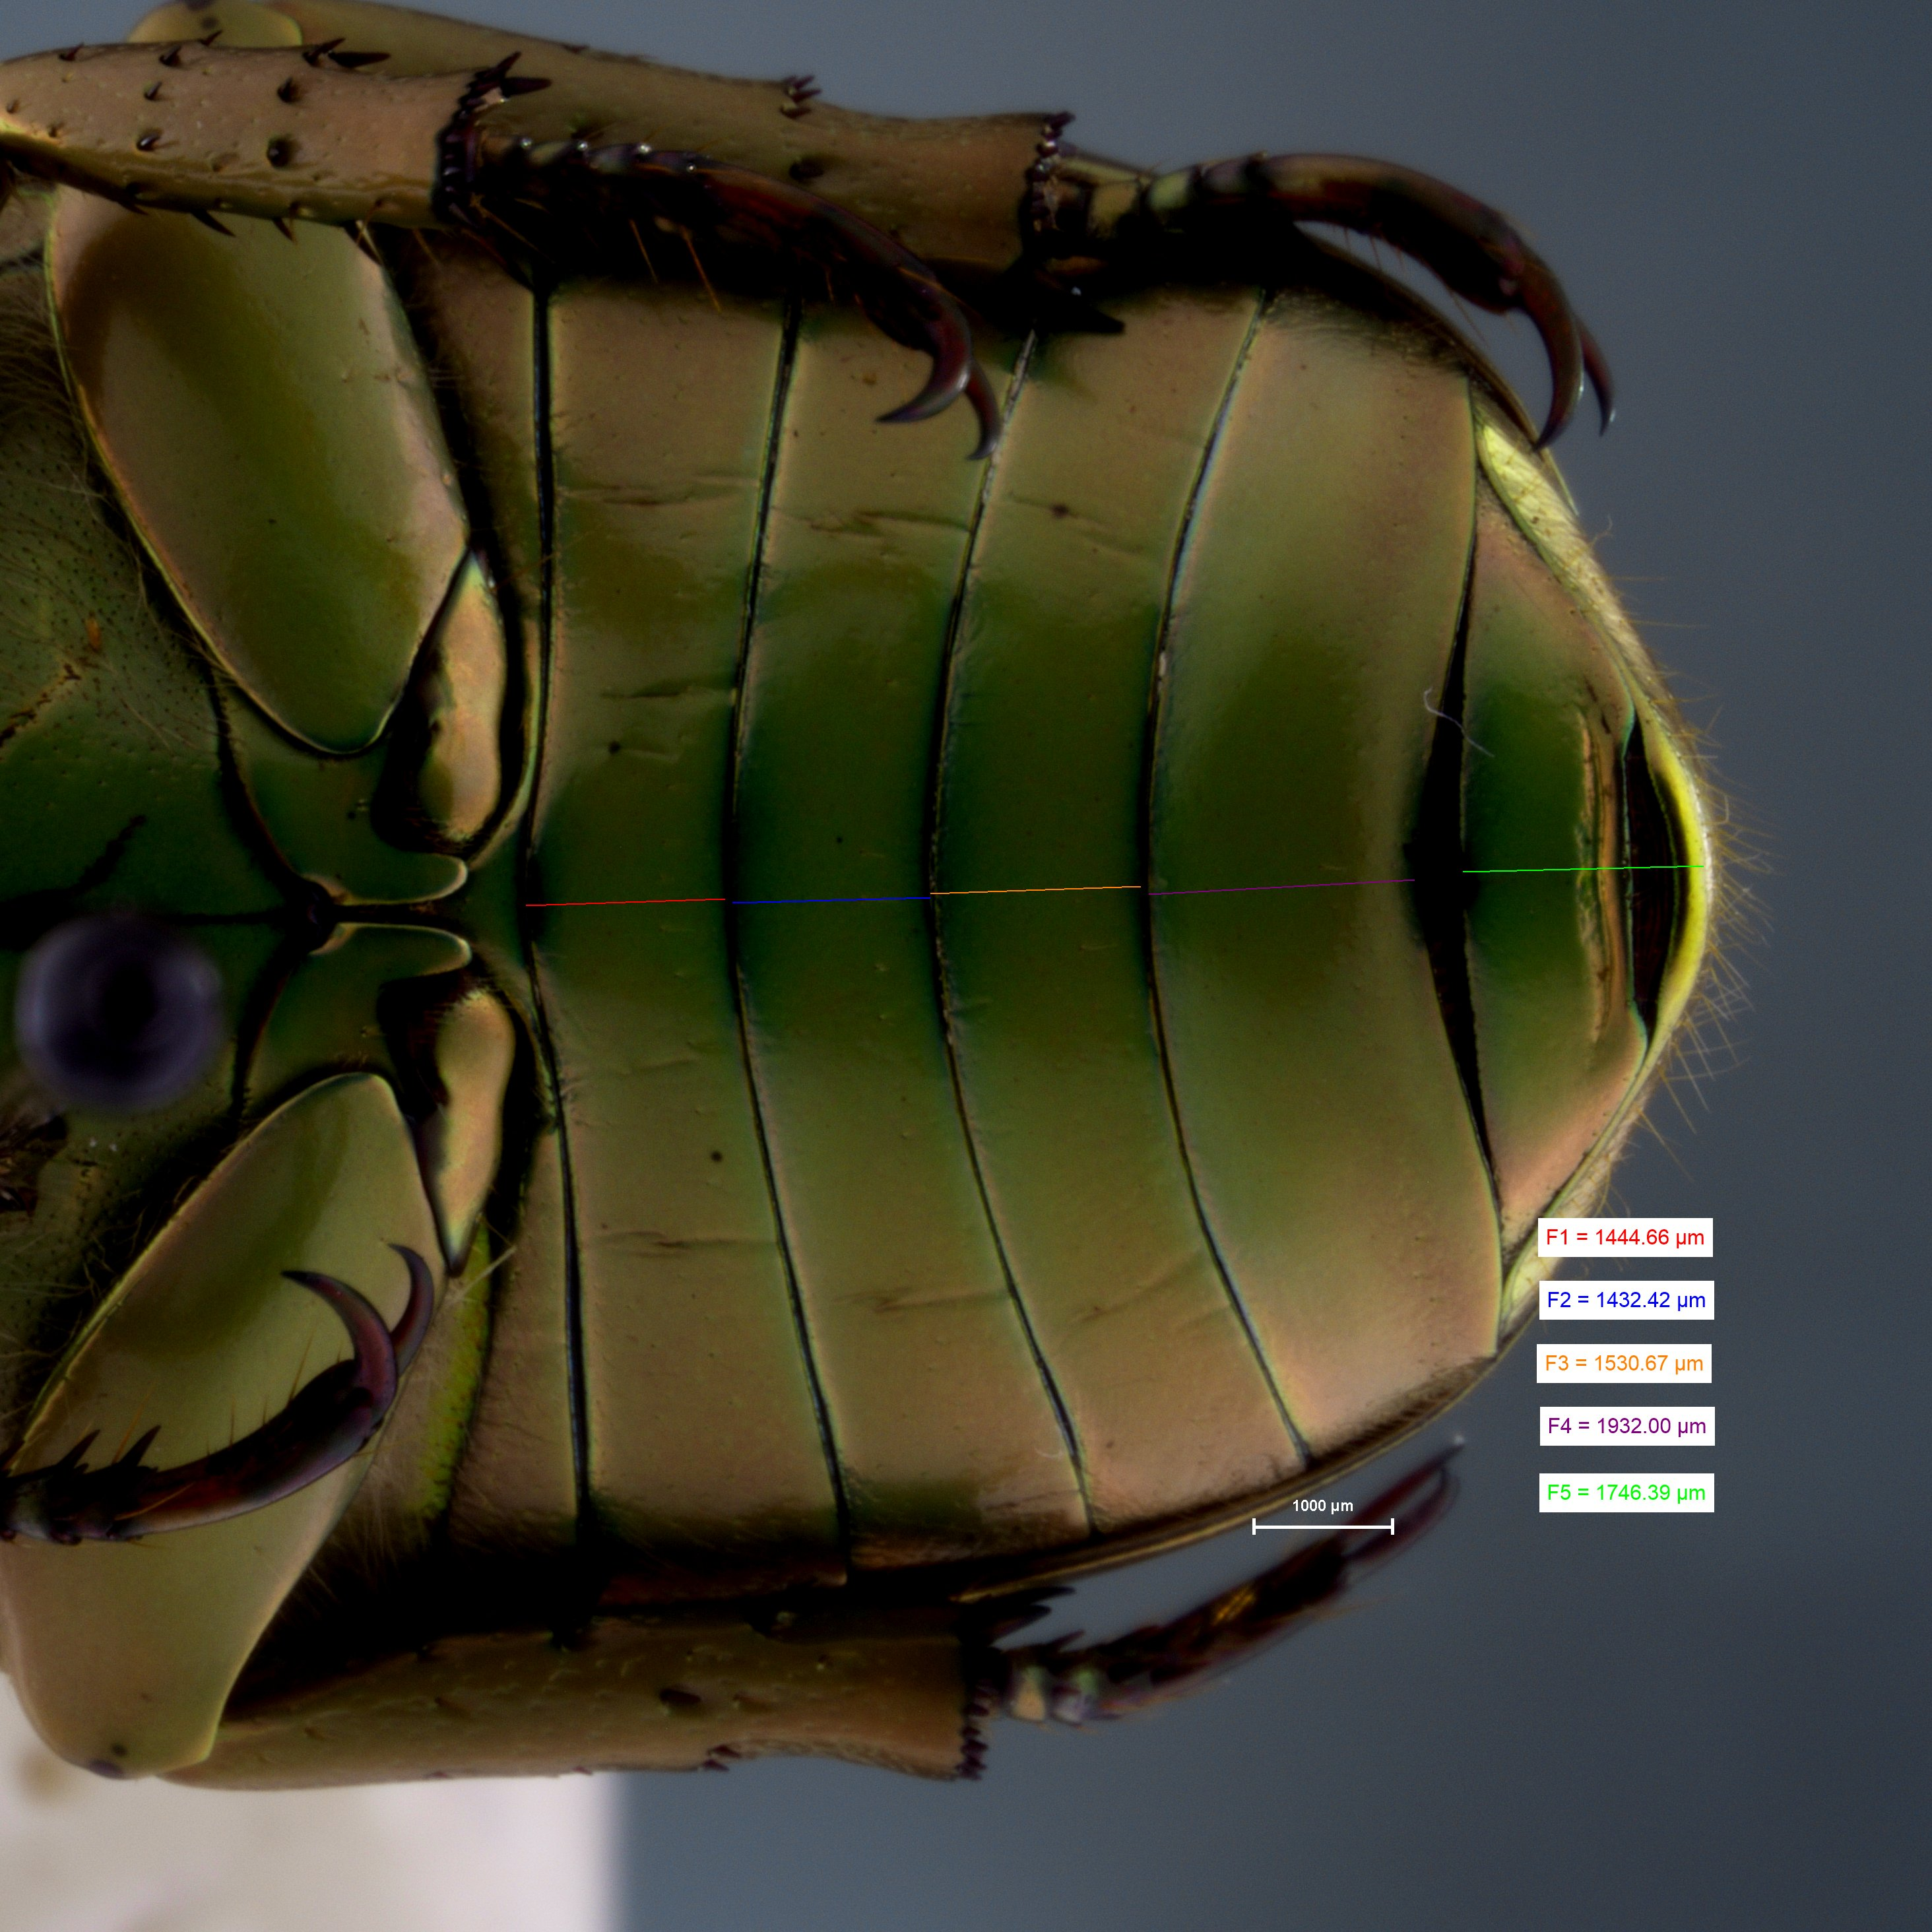
\includegraphics[width=0.5\linewidth]{images/protocol/Ventral.png}
\caption{ Metric F5}
\end{figure}

\newpage
\subsection*{Metric: A1÷A3}

A1/A3 Measure of the vertical length of beetle's head relative to its canthuses' distance width

\begin{figure}[H]
\centering
\includegraphics[width=0.7\linewidth]{images/boxplot/boxplot_A1÷A3.png}
\caption{  Boxplot and specimen distribution (superposed) for the metric  A1÷A3 by species}
\end{figure}

\noindent\textbf{Test Type:} Student's t-test \\
\noindent\textbf{Test Statistic:} 0.140 \\
\noindent\textbf{P-value:} 0.890 \\
\noindent\textbf{Interpretation:} no significant difference

\begin{figure}[H]
\centering
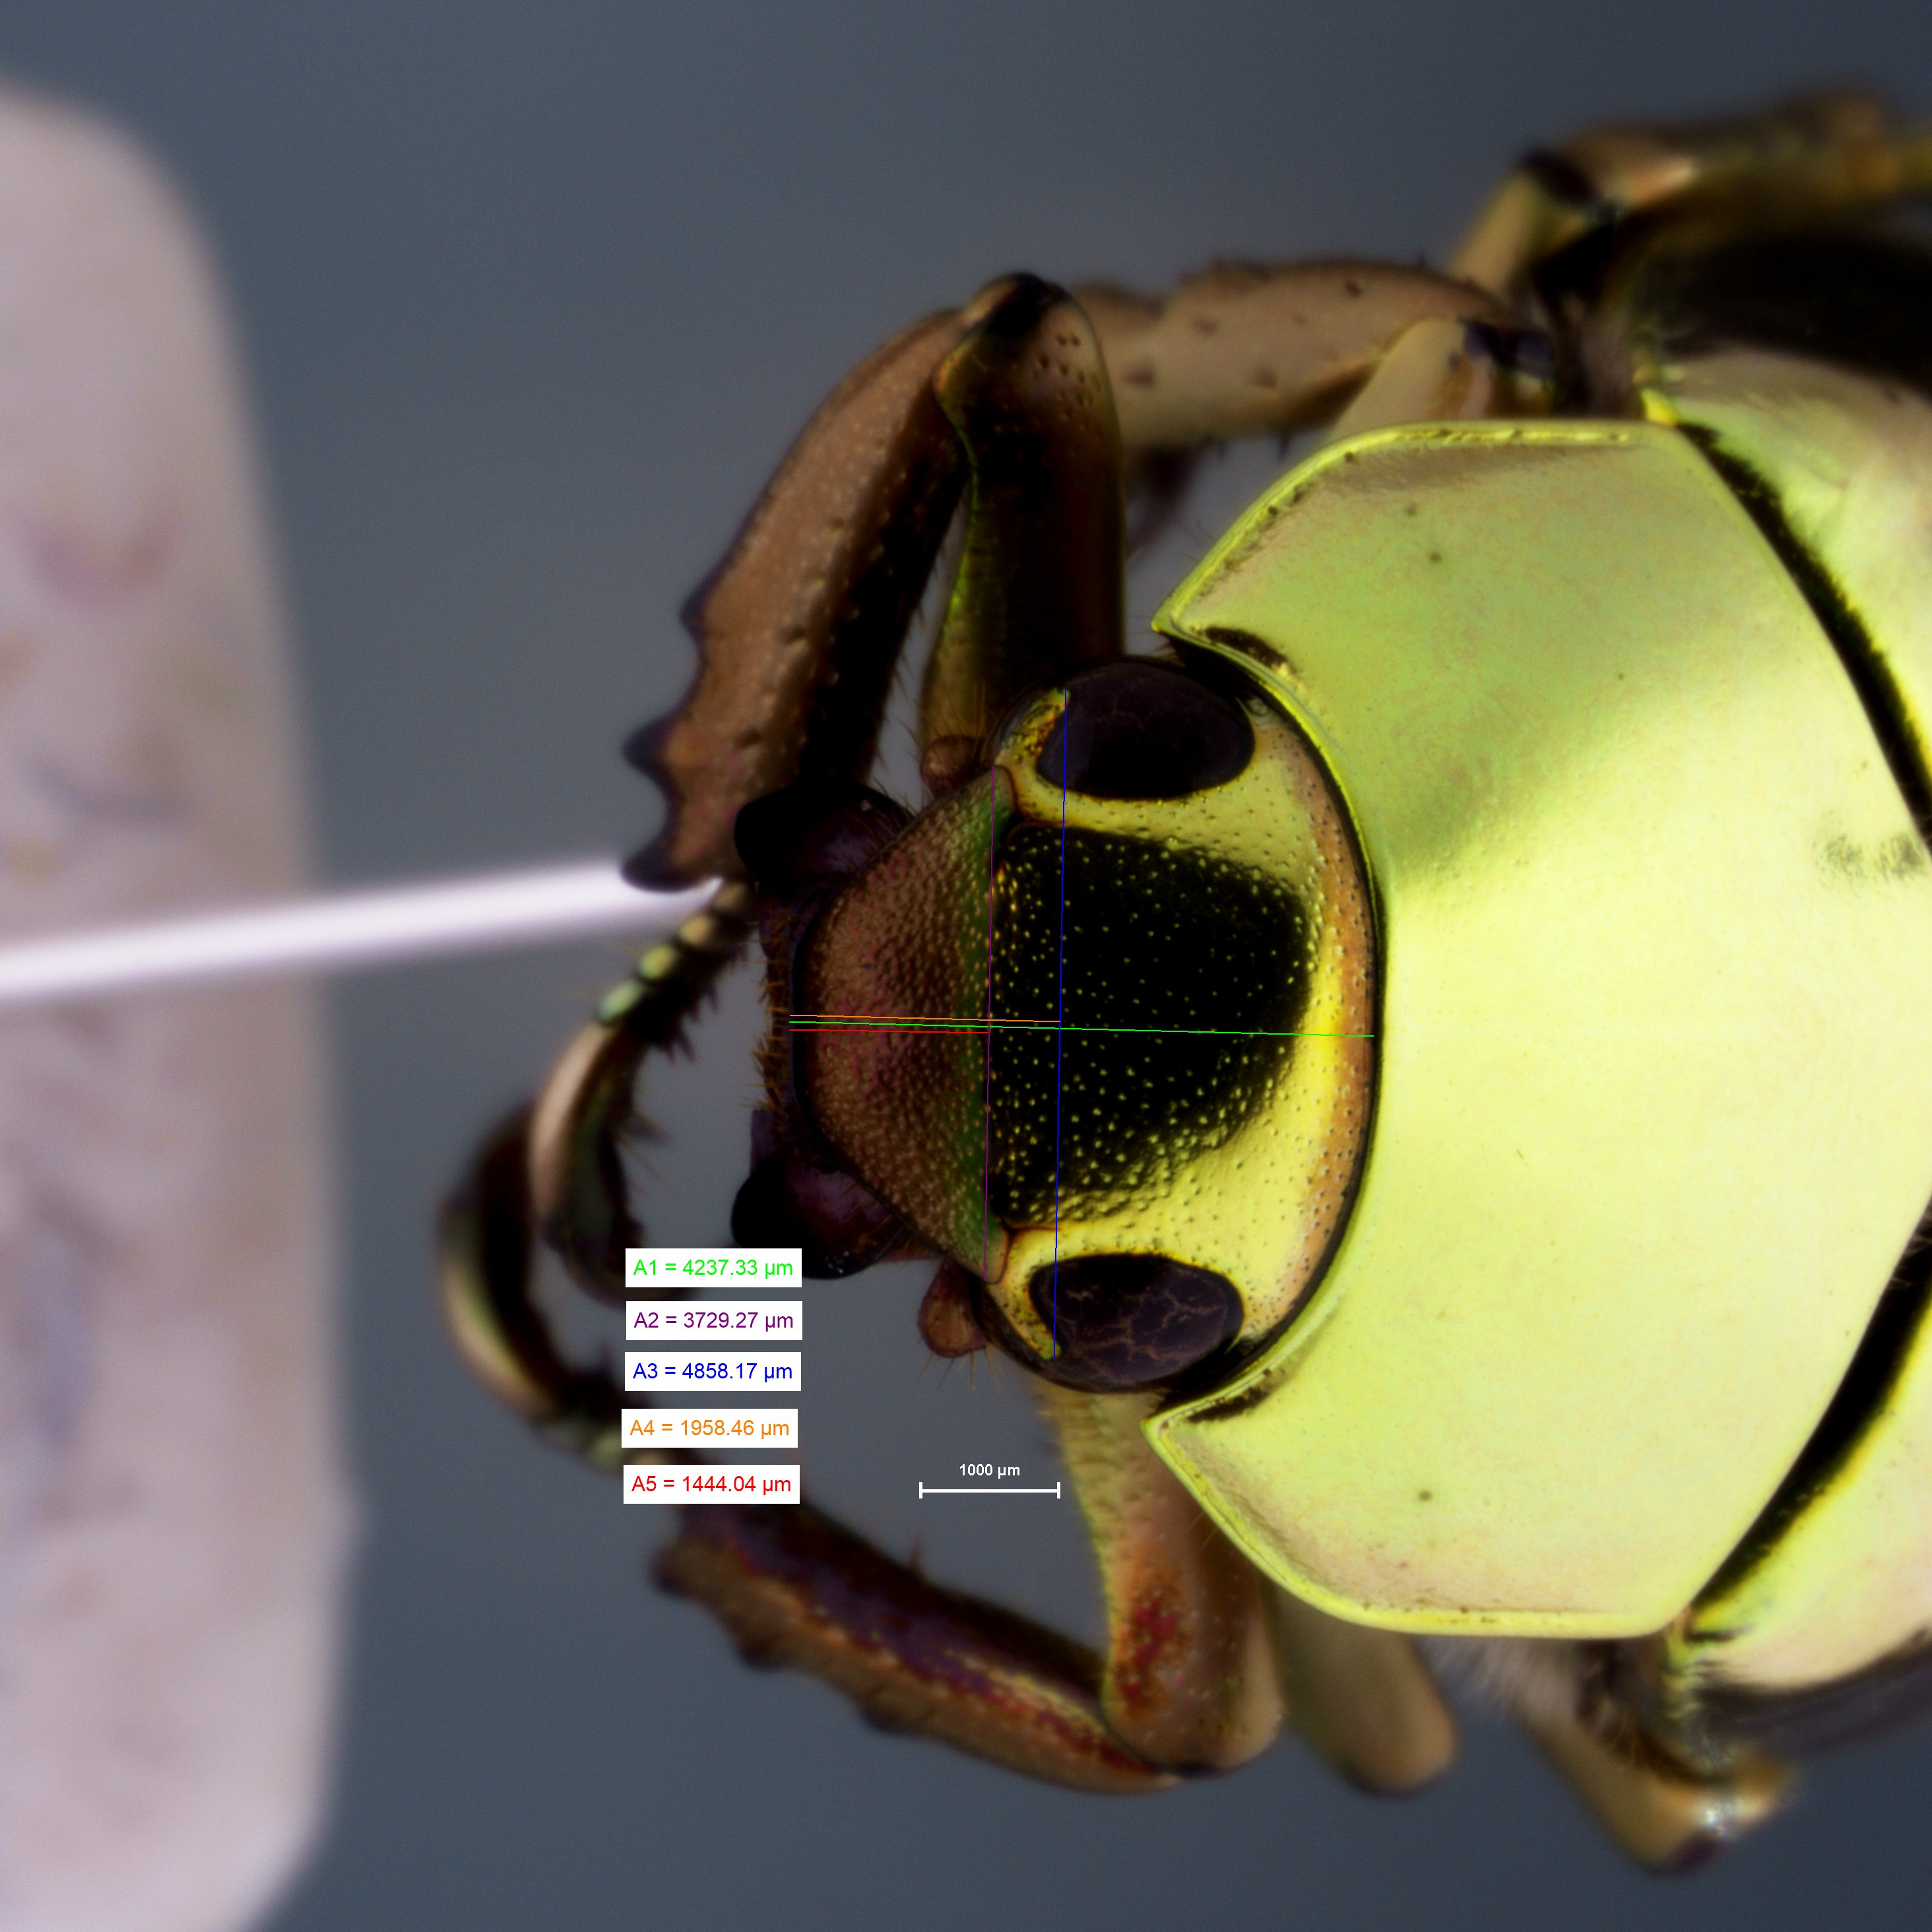
\includegraphics[width=0.5\linewidth]{images/protocol/Head.png}
\caption{ Metric A1÷A3}
\end{figure}

\newpage
\subsection*{Metric: A4÷A3}

A4/A3 Measure of the vertical length of beetle's clipeum relative to its canthuses' distance width

\begin{figure}[H]
\centering
\includegraphics[width=0.7\linewidth]{images/boxplot/boxplot_A4÷A3.png}
\caption{  Boxplot and specimen distribution (superposed) for the metric  A4÷A3 by species}
\end{figure}

\noindent\textbf{Test Type:} Mann-Whitney U test \\
\noindent\textbf{Test Statistic:} 56.000 \\
\noindent\textbf{P-value:} 0.511 \\
\noindent\textbf{Interpretation:} no significant difference

\begin{figure}[H]
\centering
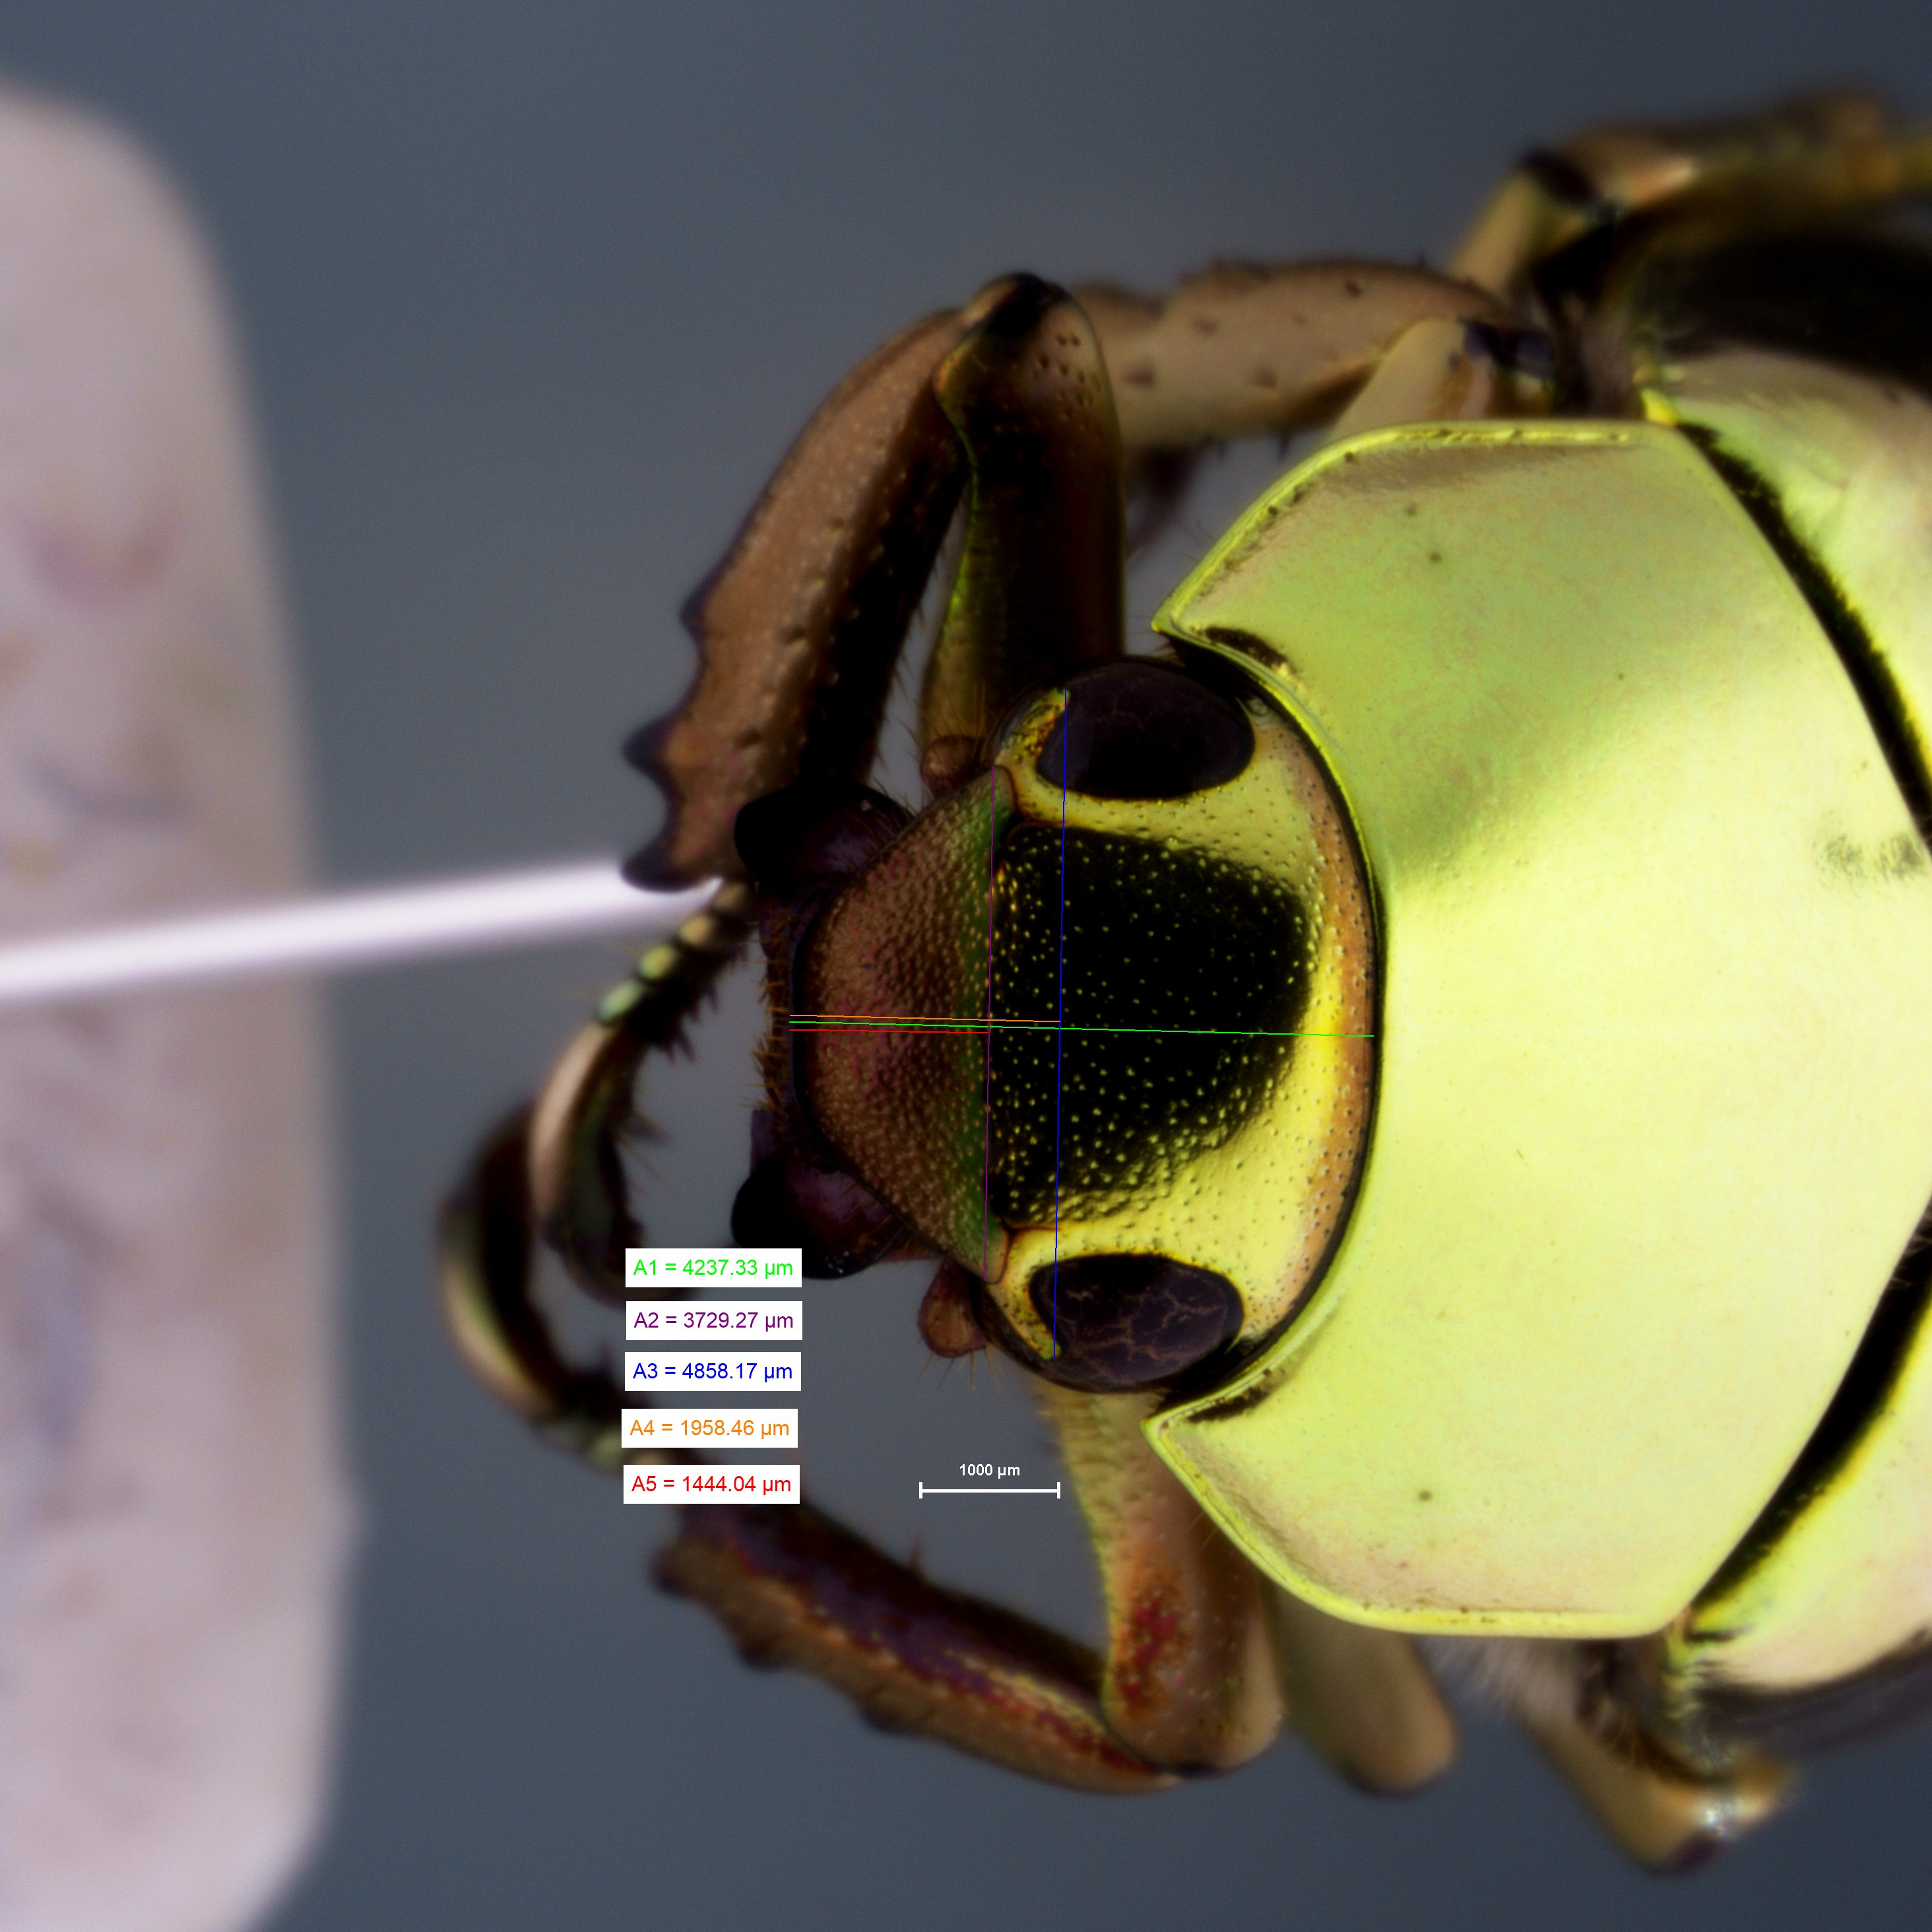
\includegraphics[width=0.5\linewidth]{images/protocol/Head.png}
\caption{ Metric A4÷A3}
\end{figure}

\newpage
\subsection*{Metric: A5÷A3}

A5/A3 Measure of the vertical length of beetle's eyes relative to its canthuses' distance width

\begin{figure}[H]
\centering
\includegraphics[width=0.7\linewidth]{images/boxplot/boxplot_A5÷A3.png}
\caption{  Boxplot and specimen distribution (superposed) for the metric  A5÷A3 by species}
\end{figure}

\noindent\textbf{Test Type:} Mann-Whitney U test \\
\noindent\textbf{Test Statistic:} 77.000 \\
\noindent\textbf{P-value:} 0.694 \\
\noindent\textbf{Interpretation:} no significant difference

\begin{figure}[H]
\centering
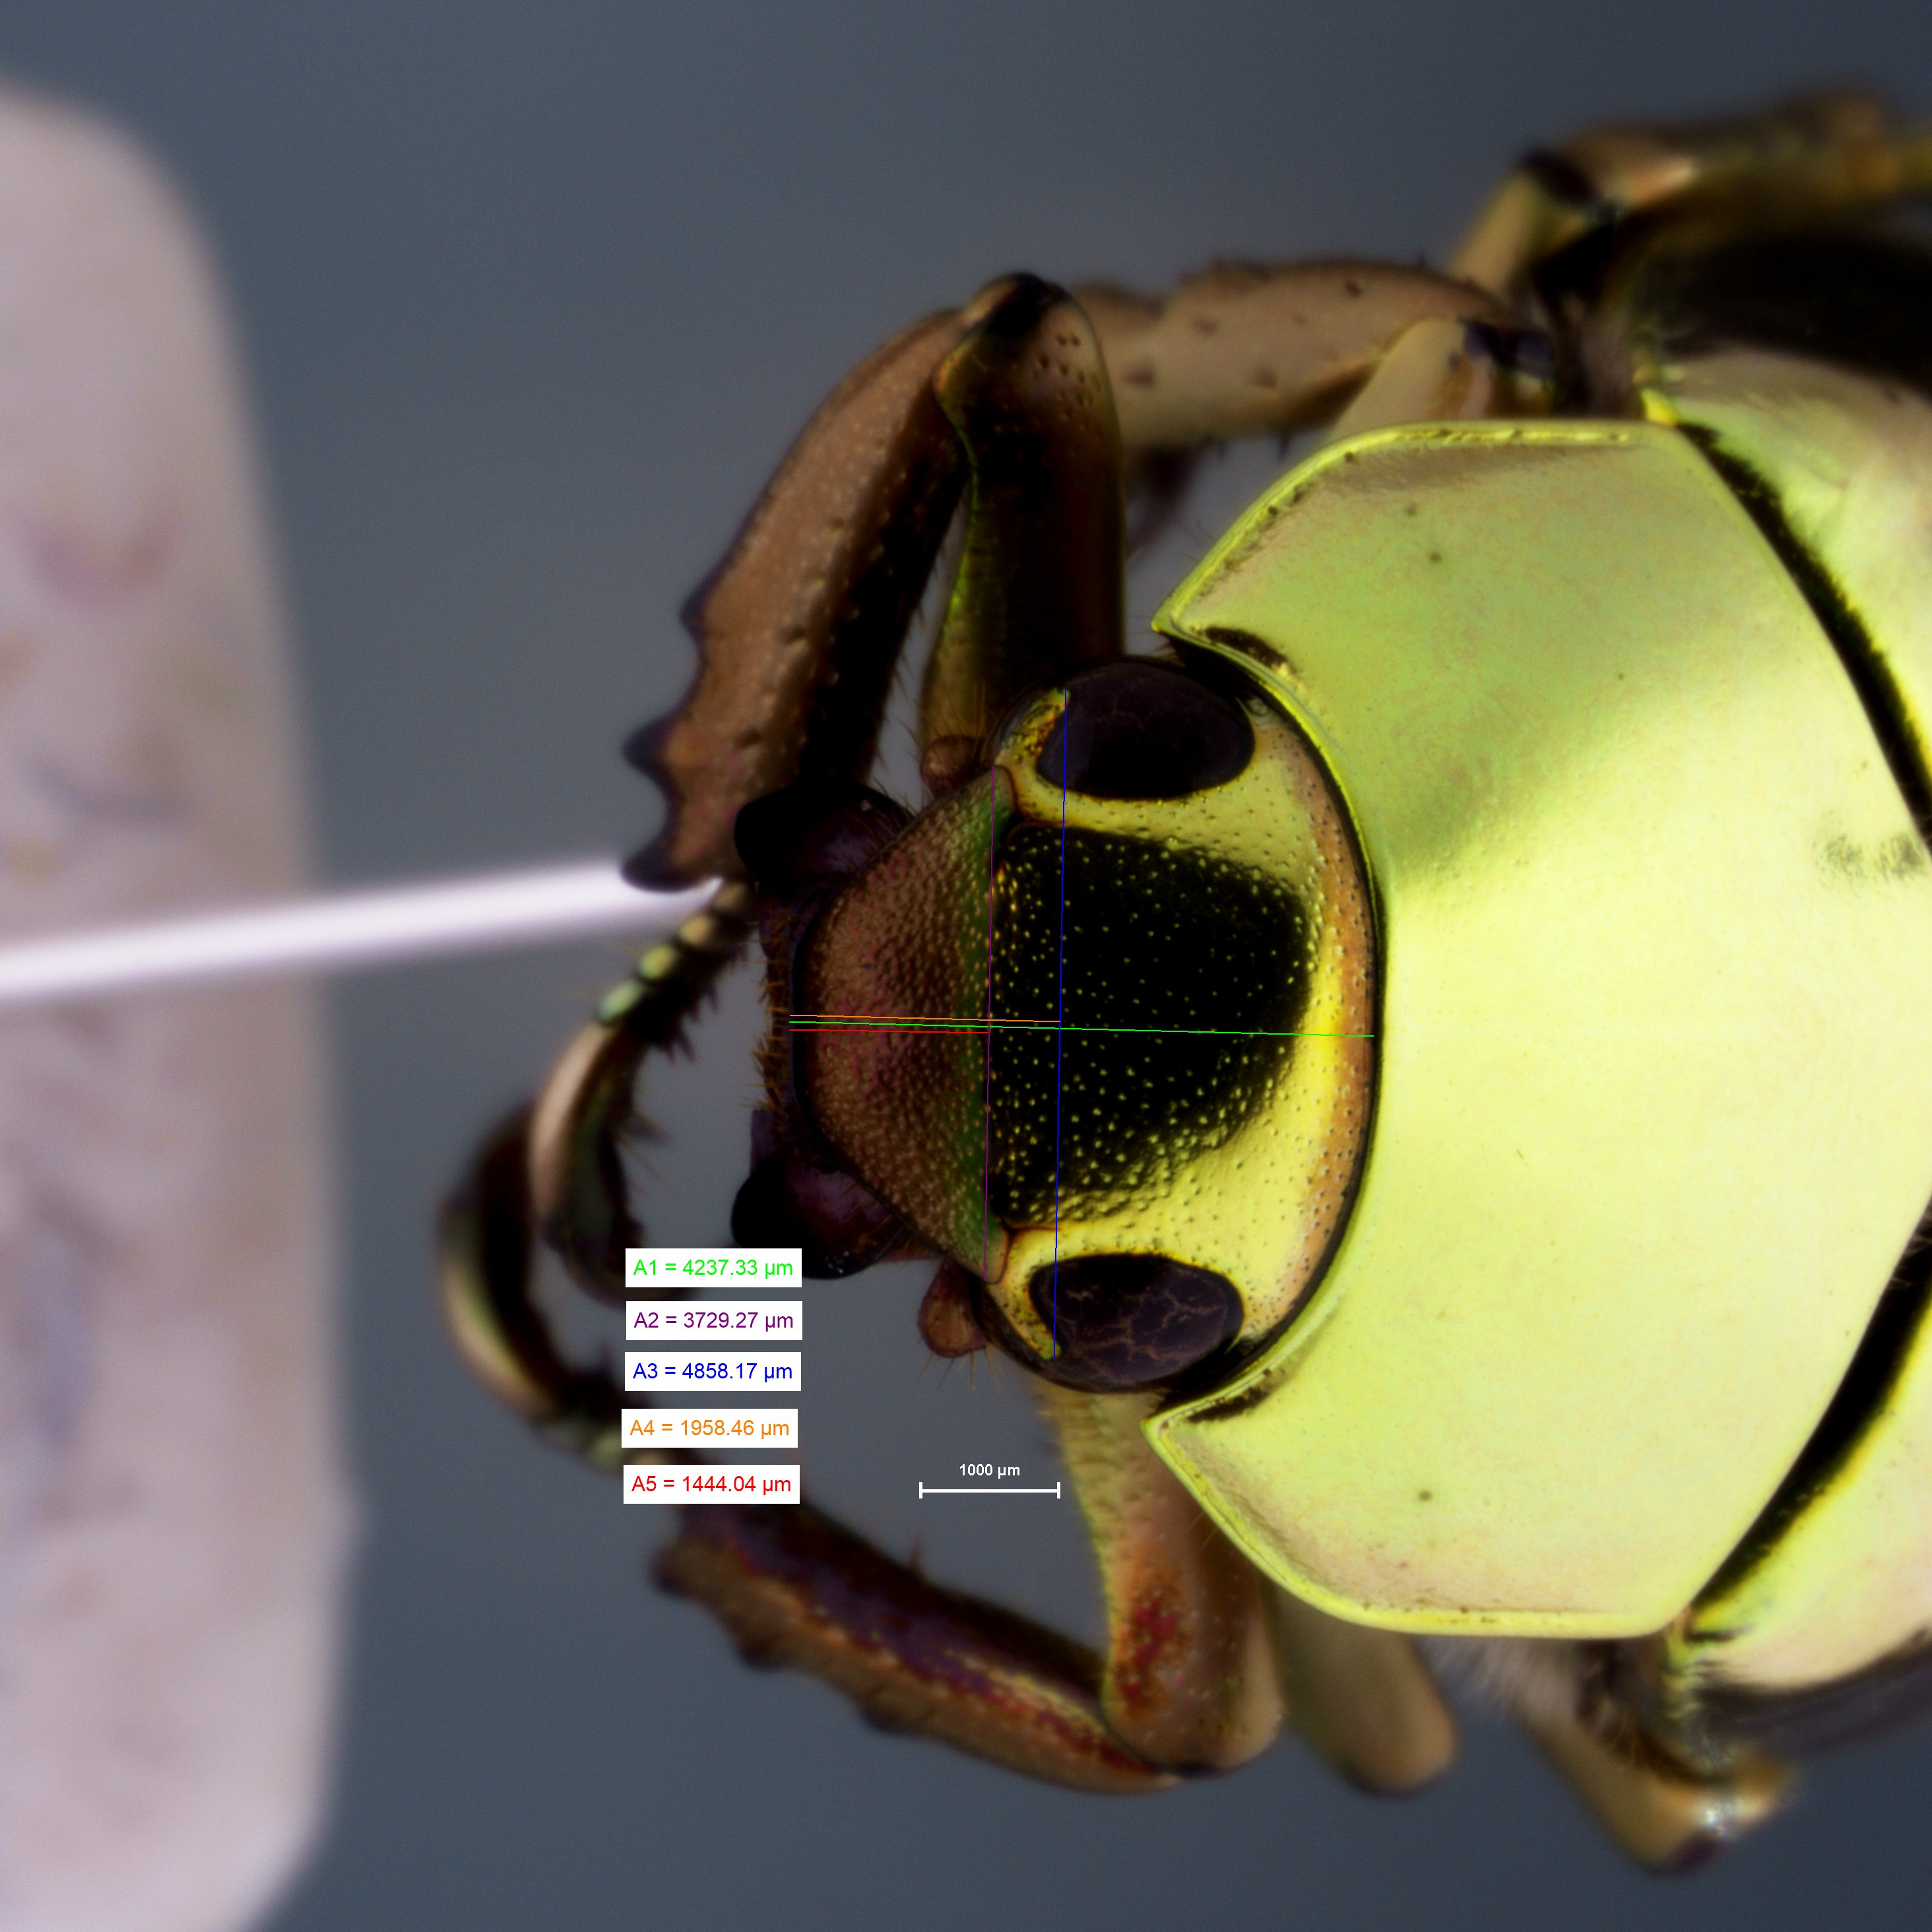
\includegraphics[width=0.5\linewidth]{images/protocol/Head.png}
\caption{ Metric A5÷A3}
\end{figure}

\newpage
\subsection*{Metric: B4÷B1}

Measure of the vertical length of the pronotum relative to its front width. B4/B1

\begin{figure}[H]
\centering
\includegraphics[width=0.7\linewidth]{images/boxplot/boxplot_B4÷B1.png}
\caption{  Boxplot and specimen distribution (superposed) for the metric  B4÷B1 by species}
\end{figure}

\noindent\textbf{Test Type:} Mann-Whitney U test \\
\noindent\textbf{Test Statistic:} 142.000 \\
\noindent\textbf{P-value:} 0.581 \\
\noindent\textbf{Interpretation:} no significant difference

\begin{figure}[H]
\centering
\includegraphics[width=0.5\linewidth]{images/protocol/Pronotum.png}
\caption{ Metric B4÷B1}
\end{figure}

\newpage
\subsection*{Metric: B4÷B2}

Measure of the vertical length of the pronotum relative to its middle width. B4/B2

\begin{figure}[H]
\centering
\includegraphics[width=0.7\linewidth]{images/boxplot/boxplot_B4÷B2.png}
\caption{  Boxplot and specimen distribution (superposed) for the metric  B4÷B2 by species}
\end{figure}

\noindent\textbf{Test Type:} Mann-Whitney U test \\
\noindent\textbf{Test Statistic:} 141.000 \\
\noindent\textbf{P-value:} 0.606 \\
\noindent\textbf{Interpretation:} no significant difference

\begin{figure}[H]
\centering
\includegraphics[width=0.5\linewidth]{images/protocol/Pronotum.png}
\caption{ Metric B4÷B2}
\end{figure}

\newpage
\subsection*{Metric: B4÷B3}

Measure of the vertical length of the pronotum relative to its back width. B4/B3

\begin{figure}[H]
\centering
\includegraphics[width=0.7\linewidth]{images/boxplot/boxplot_B4÷B3.png}
\caption{  Boxplot and specimen distribution (superposed) for the metric  B4÷B3 by species}
\end{figure}

\noindent\textbf{Test Type:} Mann-Whitney U test \\
\noindent\textbf{Test Statistic:} 134.000 \\
\noindent\textbf{P-value:} 0.797 \\
\noindent\textbf{Interpretation:} no significant difference

\begin{figure}[H]
\centering
\includegraphics[width=0.5\linewidth]{images/protocol/Pronotum.png}
\caption{ Metric B4÷B3}
\end{figure}

\newpage
\subsection*{Metric: D3÷D1}

Measure of the vertical length of the mesosternal process relative to its back width. D2/D1

\begin{figure}[H]
\centering
\includegraphics[width=0.7\linewidth]{images/boxplot/boxplot_D3÷D1.png}
\caption{  Boxplot and specimen distribution (superposed) for the metric  D3÷D1 by species}
\end{figure}

\noindent\textbf{Test Type:} Student's t-test \\
\noindent\textbf{Test Statistic:} 0.909 \\
\noindent\textbf{P-value:} 0.370 \\
\noindent\textbf{Interpretation:} no significant difference

\newpage
\subsection*{Metric: D4÷D2}

Measure of the vertical length of the mesosternal process down to the middle dark stripe  relative to its middle width. D2/D3

\begin{figure}[H]
\centering
\includegraphics[width=0.7\linewidth]{images/boxplot/boxplot_D4÷D2.png}
\caption{  Boxplot and specimen distribution (superposed) for the metric  D4÷D2 by species}
\end{figure}

\noindent\textbf{Test Type:} Student's t-test \\
\noindent\textbf{Test Statistic:} -2.646 \\
\noindent\textbf{P-value:} 0.013 \\
\noindent\textbf{Interpretation:} significant difference

\newpage
\subsection*{Metric: E1÷E2}

Measure of how square the prosternal plate is. Front width back width ratio E1/E2

\begin{figure}[H]
\centering
\includegraphics[width=0.7\linewidth]{images/boxplot/boxplot_E1÷E2.png}
\caption{  Boxplot and specimen distribution (superposed) for the metric  E1÷E2 by species}
\end{figure}

\noindent\textbf{Test Type:} Student's t-test \\
\noindent\textbf{Test Statistic:} -1.968 \\
\noindent\textbf{P-value:} 0.058 \\
\noindent\textbf{Interpretation:} no significant difference

\begin{figure}[H]
\centering
\includegraphics[width=0.5\linewidth]{images/protocol/Prosternal_process.png}
\caption{ Metric E1÷E2}
\end{figure}

\newpage
